% =====================================================================
% MLLB-DL report of Oriana Ferraz De Jesus (experimental design, PyTorch,
% training, evaluation, reproducibility).
% Compile from report/:  pdflatex oriana_mllb && bibtex oriana_mllb && pdflatex x2
% Shared parts: common/ (preamble, floats, code excerpts, contributions); text: oriana/.
% =====================================================================
\documentclass[11pt]{article}
% =====================================================================
% Shared preamble of the four DL reports (PRDL-DL and MLLB-DL of each author).
% Written once; each main file (report/<author>_<course>.tex) does
%     \documentclass[11pt]{article}
%     % =====================================================================
% Shared preamble of the four DL reports (PRDL-DL and MLLB-DL of each author).
% Written once; each main file (report/<author>_<course>.tex) does
%     \documentclass[11pt]{article}
%     % =====================================================================
% Shared preamble of the four DL reports (PRDL-DL and MLLB-DL of each author).
% Written once; each main file (report/<author>_<course>.tex) does
%     \documentclass[11pt]{article}
%     \input{common/preamble}
% and is compiled from the folder report/, so every path below is relative
% to report/ (also on Overleaf: upload report/ and choose the main file).
% Style taken from the ML reports (contexto_DL/ML_ref_*_main.tex.txt).
% =====================================================================

% ---------- Packages ----------
\usepackage[a4paper,margin=2.5cm]{geometry}
\usepackage[utf8]{inputenc}
\usepackage[T1]{fontenc}
\usepackage{lmodern}
\usepackage{amsmath,amssymb}
\usepackage{graphicx}
\usepackage{xcolor}
\usepackage{tabularx}
\usepackage{booktabs}
\usepackage{enumitem}
\usepackage[explicit]{titlesec}
\usepackage{fancyhdr}
\usepackage{caption}
\usepackage{float}
\usepackage{array}
\usepackage{adjustbox}   % tables shrink to the text width only when wider
\usepackage{listings}
\usepackage{siunitx}
\usepackage{cite}
\usepackage{hyperref}
\hypersetup{hidelinks}

% ---------- Colours ----------
\definecolor{etsitorange}{RGB}{237,125,49}
\definecolor{etsitblue}{RGB}{31,73,125}
\definecolor{codebg}{RGB}{245,245,245}

% ---------- Code listings (MLLB) ----------
\lstset{
  language=Python,
  backgroundcolor=\color{codebg},
  basicstyle=\ttfamily\footnotesize,
  breaklines=true,
  frame=single,
  columns=fullflexible,
  keepspaces=true,
  numbers=left,
  numberstyle=\tiny\color{gray},
  keywordstyle=\color{etsitblue}\bfseries,
  commentstyle=\color{gray}\itshape,
  showstringspaces=false
}

% ---------- Section banners (orange bar, as in the course template) ----------
\titleformat{\section}
  {\bfseries\Large\color{white}}
  {}{0pt}
  {\colorbox{etsitorange}{\parbox{\dimexpr\textwidth-4\fboxsep-12pt\relax}{\centering\thesection.\ #1}}}
\titlespacing*{\section}{0pt}{18pt}{12pt}
\titleformat{name=\section,numberless}
  {\bfseries\Large\color{white}}
  {}{0pt}
  {\colorbox{etsitorange}{\parbox{\dimexpr\textwidth-4\fboxsep-12pt\relax}{\centering#1}}}
\titlespacing*{name=\section,numberless}{0pt}{18pt}{12pt}
\titleformat{\subsection}{\bfseries\large}{\thesubsection.}{0.5em}{#1}
\titlespacing*{\subsection}{0pt}{12pt}{6pt}
\titleformat{\subsubsection}{\bfseries\normalsize}{\thesubsubsection}{0.5em}{#1}
\titlespacing*{\subsubsection}{0pt}{10pt}{4pt}

% Appendix banner (no number)
\newcommand{\appendixbanner}[1]{%
  \colorbox{etsitorange}{\parbox{\dimexpr\textwidth-4\fboxsep-12pt\relax}{\centering\bfseries\Large\color{white} #1}}%
  \vspace{12pt}}

\renewcommand{\contentsname}{CONTENTS}
\renewcommand{\listtablename}{LIST OF TABLES}
\renewcommand{\listfigurename}{LIST OF FIGURES}

\pagestyle{fancy}
\fancyhf{}
\renewcommand{\headrulewidth}{0pt}
\fancyfoot[C]{\thepage}

\captionsetup{font=small,labelfont=bf}
\graphicspath{{figures/}}
\setlength{\emergencystretch}{2em}

% ---------- Numbers ----------
% Every measured number is a macro generated from results/logs/*.json by
% report/make_numbers.py; published results come from report/published.json.
\input{numbers}

% A claim without a checked quote would be tagged with this macro; the final
% version must contain none (checked before delivery).
\newcommand{\todoverify}[1]{\textcolor{red}{\,\textsf{\footnotesize[verify: #1]}}}

% ---------- Helpers ----------
% Rounded display of a number macro (only for macros without a thousands
% separator), e.g. \intval{\edaAgeMedianNORM} -> 54; the value still comes from the log.
\newcommand{\intval}[1]{\num[round-mode=places,round-precision=0]{#1}}
\newcommand{\onedec}[1]{\num[round-mode=places,round-precision=1]{#1}}
% File or code name in typewriter font (url's \path breaks long names at / . _)
\newcommand{\file}[1]{\path{#1}}
% Report kind: \prdltrue in PRDL mains, \prdlfalse in MLLB mains
\newif\ifprdl

% Cover page: \reportcover{course}{report title}{author}{date}
\newcommand{\reportcover}[4]{%
\begin{titlepage}
\centering
\vspace*{1cm}
\IfFileExists{figures/etsit_logo.jpeg}{
\includegraphics[width=0.4\textwidth]{figures/etsit_logo.jpeg}\par}{}
\vspace{1.5cm}
{\color{etsitblue}\bfseries\Large Course:}\par
\vspace{0.5cm}
{\bfseries\huge #1}\par
\vspace{1cm}
{\Large Deep Learning Report}\par
{\bfseries\Large #2}\par
\vspace{0.5cm}
\rule{0.7\textwidth}{0.4pt}\par
\vspace{0.5cm}
{\large Master in Signal Theory and Communications (MUTSC), ETSIT -- Universidad Polit\'ecnica de Madrid}\par
\vspace{2.5cm}
\large Name: \underline{\hspace{2mm}#3\hspace{2mm}}\par
\vspace{0.3cm}
\large Team: Oriana Andrea Ferraz De Jesus and Mar\'ia Mart\'inez Garc\'ia-Tahe\~no\par
\vspace{0.5cm}
\hfill Date: \underline{\hspace{2mm}#4\hspace{2mm}}\par
\vfill
{\small Code and results: \url{https://github.com/orianafe16/ptbxl-DL}}\par
\end{titlepage}}

% and is compiled from the folder report/, so every path below is relative
% to report/ (also on Overleaf: upload report/ and choose the main file).
% Style taken from the ML reports (contexto_DL/ML_ref_*_main.tex.txt).
% =====================================================================

% ---------- Packages ----------
\usepackage[a4paper,margin=2.5cm]{geometry}
\usepackage[utf8]{inputenc}
\usepackage[T1]{fontenc}
\usepackage{lmodern}
\usepackage{amsmath,amssymb}
\usepackage{graphicx}
\usepackage{xcolor}
\usepackage{tabularx}
\usepackage{booktabs}
\usepackage{enumitem}
\usepackage[explicit]{titlesec}
\usepackage{fancyhdr}
\usepackage{caption}
\usepackage{float}
\usepackage{array}
\usepackage{adjustbox}   % tables shrink to the text width only when wider
\usepackage{listings}
\usepackage{siunitx}
\usepackage{cite}
\usepackage{hyperref}
\hypersetup{hidelinks}

% ---------- Colours ----------
\definecolor{etsitorange}{RGB}{237,125,49}
\definecolor{etsitblue}{RGB}{31,73,125}
\definecolor{codebg}{RGB}{245,245,245}

% ---------- Code listings (MLLB) ----------
\lstset{
  language=Python,
  backgroundcolor=\color{codebg},
  basicstyle=\ttfamily\footnotesize,
  breaklines=true,
  frame=single,
  columns=fullflexible,
  keepspaces=true,
  numbers=left,
  numberstyle=\tiny\color{gray},
  keywordstyle=\color{etsitblue}\bfseries,
  commentstyle=\color{gray}\itshape,
  showstringspaces=false
}

% ---------- Section banners (orange bar, as in the course template) ----------
\titleformat{\section}
  {\bfseries\Large\color{white}}
  {}{0pt}
  {\colorbox{etsitorange}{\parbox{\dimexpr\textwidth-4\fboxsep-12pt\relax}{\centering\thesection.\ #1}}}
\titlespacing*{\section}{0pt}{18pt}{12pt}
\titleformat{name=\section,numberless}
  {\bfseries\Large\color{white}}
  {}{0pt}
  {\colorbox{etsitorange}{\parbox{\dimexpr\textwidth-4\fboxsep-12pt\relax}{\centering#1}}}
\titlespacing*{name=\section,numberless}{0pt}{18pt}{12pt}
\titleformat{\subsection}{\bfseries\large}{\thesubsection.}{0.5em}{#1}
\titlespacing*{\subsection}{0pt}{12pt}{6pt}
\titleformat{\subsubsection}{\bfseries\normalsize}{\thesubsubsection}{0.5em}{#1}
\titlespacing*{\subsubsection}{0pt}{10pt}{4pt}

% Appendix banner (no number)
\newcommand{\appendixbanner}[1]{%
  \colorbox{etsitorange}{\parbox{\dimexpr\textwidth-4\fboxsep-12pt\relax}{\centering\bfseries\Large\color{white} #1}}%
  \vspace{12pt}}

\renewcommand{\contentsname}{CONTENTS}
\renewcommand{\listtablename}{LIST OF TABLES}
\renewcommand{\listfigurename}{LIST OF FIGURES}

\pagestyle{fancy}
\fancyhf{}
\renewcommand{\headrulewidth}{0pt}
\fancyfoot[C]{\thepage}

\captionsetup{font=small,labelfont=bf}
\graphicspath{{figures/}}
\setlength{\emergencystretch}{2em}

% ---------- Numbers ----------
% Every measured number is a macro generated from results/logs/*.json by
% report/make_numbers.py; published results come from report/published.json.
% numbers.tex: generated by report/make_numbers.py on 2026-11-20 19:44. Do not edit by hand.
% Sources:
%   eda: results/logs/eda.json (created 2026-11-20T17:53:34, git 8441284)
%   trivial: results/logs/trivial_e2e_s42_20261120-183809.json (created 2026-11-20T18:39:15, git f090231, uncommitted changes)
%   dense: results/logs/dense_summary.json (created 2026-11-20T19:44:51, git fcc3c3b, uncommitted changes)

% ---- eda: eda
% eda: n_records_all
\newcommand{\edaNRecordsAll}{21{,}799}
% eda: n_patients_all
\newcommand{\edaNPatientsAll}{18{,}869}
% eda: n_labelled_all
\newcommand{\edaNLabelledAll}{21{,}388}
% eda: n_records_train
\newcommand{\edaNRecordsTrain}{17{,}418}
% eda: n_patients_train
\newcommand{\edaNPatientsTrain}{15{,}023}
% eda: n_labelled_train
\newcommand{\edaNLabelledTrain}{17{,}084}
% eda: n_records_val
\newcommand{\edaNRecordsVal}{2{,}183}
% eda: n_patients_val
\newcommand{\edaNPatientsVal}{1{,}942}
% eda: n_labelled_val
\newcommand{\edaNLabelledVal}{2{,}146}
% eda: n_records_test
\newcommand{\edaNRecordsTest}{2{,}198}
% eda: n_patients_test
\newcommand{\edaNPatientsTest}{1{,}904}
% eda: n_labelled_test
\newcommand{\edaNLabelledTest}{2{,}158}
% eda: n_nosuper_all
\newcommand{\edaNNosuperAll}{411}
% eda: n_nosuper_pacemaker_field
\newcommand{\edaNNosuperPacemakerField}{277}
% eda: n_nosuper_with_rhythm_code
\newcommand{\edaNNosuperWithRhythmCode}{409}
% eda: n_nosuper_with_form_code
\newcommand{\edaNNosuperWithFormCode}{41}
% eda: n_nosuper_rhythm_only
\newcommand{\edaNNosuperRhythmOnly}{370}
% eda: n_nosuper_train
\newcommand{\edaNNosuperTrain}{334}
% eda: n_nosuper_val
\newcommand{\edaNNosuperVal}{37}
% eda: n_nosuper_test
\newcommand{\edaNNosuperTest}{40}
% eda: count_all_NORM
\newcommand{\edaCountAllNORM}{9{,}514}
% eda: prev_all_NORM
\newcommand{\edaPrevAllNORM}{0.445}
% eda: prev_all_NORM
\newcommand{\edaPrevAllNORMPct}{44.5\%}
% eda: count_all_MI
\newcommand{\edaCountAllMI}{5{,}469}
% eda: prev_all_MI
\newcommand{\edaPrevAllMI}{0.256}
% eda: prev_all_MI
\newcommand{\edaPrevAllMIPct}{25.6\%}
% eda: count_all_STTC
\newcommand{\edaCountAllSTTC}{5{,}235}
% eda: prev_all_STTC
\newcommand{\edaPrevAllSTTC}{0.245}
% eda: prev_all_STTC
\newcommand{\edaPrevAllSTTCPct}{24.5\%}
% eda: count_all_CD
\newcommand{\edaCountAllCD}{4{,}898}
% eda: prev_all_CD
\newcommand{\edaPrevAllCD}{0.229}
% eda: prev_all_CD
\newcommand{\edaPrevAllCDPct}{22.9\%}
% eda: count_all_HYP
\newcommand{\edaCountAllHYP}{2{,}649}
% eda: prev_all_HYP
\newcommand{\edaPrevAllHYP}{0.124}
% eda: prev_all_HYP
\newcommand{\edaPrevAllHYPPct}{12.4\%}
% eda: count_train_NORM
\newcommand{\edaCountTrainNORM}{7{,}596}
% eda: prev_train_NORM
\newcommand{\edaPrevTrainNORM}{0.445}
% eda: prev_train_NORM
\newcommand{\edaPrevTrainNORMPct}{44.5\%}
% eda: count_train_MI
\newcommand{\edaCountTrainMI}{4{,}379}
% eda: prev_train_MI
\newcommand{\edaPrevTrainMI}{0.256}
% eda: prev_train_MI
\newcommand{\edaPrevTrainMIPct}{25.6\%}
% eda: count_train_STTC
\newcommand{\edaCountTrainSTTC}{4{,}186}
% eda: prev_train_STTC
\newcommand{\edaPrevTrainSTTC}{0.245}
% eda: prev_train_STTC
\newcommand{\edaPrevTrainSTTCPct}{24.5\%}
% eda: count_train_CD
\newcommand{\edaCountTrainCD}{3{,}907}
% eda: prev_train_CD
\newcommand{\edaPrevTrainCD}{0.229}
% eda: prev_train_CD
\newcommand{\edaPrevTrainCDPct}{22.9\%}
% eda: count_train_HYP
\newcommand{\edaCountTrainHYP}{2{,}119}
% eda: prev_train_HYP
\newcommand{\edaPrevTrainHYP}{0.124}
% eda: prev_train_HYP
\newcommand{\edaPrevTrainHYPPct}{12.4\%}
% eda: count_val_NORM
\newcommand{\edaCountValNORM}{955}
% eda: prev_val_NORM
\newcommand{\edaPrevValNORM}{0.445}
% eda: prev_val_NORM
\newcommand{\edaPrevValNORMPct}{44.5\%}
% eda: count_val_MI
\newcommand{\edaCountValMI}{540}
% eda: prev_val_MI
\newcommand{\edaPrevValMI}{0.252}
% eda: prev_val_MI
\newcommand{\edaPrevValMIPct}{25.2\%}
% eda: count_val_STTC
\newcommand{\edaCountValSTTC}{528}
% eda: prev_val_STTC
\newcommand{\edaPrevValSTTC}{0.246}
% eda: prev_val_STTC
\newcommand{\edaPrevValSTTCPct}{24.6\%}
% eda: count_val_CD
\newcommand{\edaCountValCD}{495}
% eda: prev_val_CD
\newcommand{\edaPrevValCD}{0.231}
% eda: prev_val_CD
\newcommand{\edaPrevValCDPct}{23.1\%}
% eda: count_val_HYP
\newcommand{\edaCountValHYP}{268}
% eda: prev_val_HYP
\newcommand{\edaPrevValHYP}{0.125}
% eda: prev_val_HYP
\newcommand{\edaPrevValHYPPct}{12.5\%}
% eda: count_test_NORM
\newcommand{\edaCountTestNORM}{963}
% eda: prev_test_NORM
\newcommand{\edaPrevTestNORM}{0.446}
% eda: prev_test_NORM
\newcommand{\edaPrevTestNORMPct}{44.6\%}
% eda: count_test_MI
\newcommand{\edaCountTestMI}{550}
% eda: prev_test_MI
\newcommand{\edaPrevTestMI}{0.255}
% eda: prev_test_MI
\newcommand{\edaPrevTestMIPct}{25.5\%}
% eda: count_test_STTC
\newcommand{\edaCountTestSTTC}{521}
% eda: prev_test_STTC
\newcommand{\edaPrevTestSTTC}{0.241}
% eda: prev_test_STTC
\newcommand{\edaPrevTestSTTCPct}{24.1\%}
% eda: count_test_CD
\newcommand{\edaCountTestCD}{496}
% eda: prev_test_CD
\newcommand{\edaPrevTestCD}{0.230}
% eda: prev_test_CD
\newcommand{\edaPrevTestCDPct}{23.0\%}
% eda: count_test_HYP
\newcommand{\edaCountTestHYP}{262}
% eda: prev_test_HYP
\newcommand{\edaPrevTestHYP}{0.121}
% eda: prev_test_HYP
\newcommand{\edaPrevTestHYPPct}{12.1\%}
% eda: imbalance_ratio_train
\newcommand{\edaImbalanceRatioTrain}{3.585}
% eda: n_with_1_labels
\newcommand{\edaNWithOneLabels}{16{,}244}
% eda: n_with_2_labels
\newcommand{\edaNWithTwoLabels}{4{,}068}
% eda: n_with_3_labels
\newcommand{\edaNWithThreeLabels}{919}
% eda: n_with_4_labels
\newcommand{\edaNWithFourLabels}{157}
% eda: frac_multilabel_all
\newcommand{\edaFracMultilabelAll}{0.241}
% eda: frac_multilabel_all
\newcommand{\edaFracMultilabelAllPct}{24.1\%}
% eda: n_norm_with_other
\newcommand{\edaNNormWithOther}{445}
% eda: n_combinations
\newcommand{\edaNCombinations}{22}
% eda: max_fold_prev_gap_pp
\newcommand{\edaMaxFoldPrevGapPp}{1.610}
% eda: n_age_over89_all
\newcommand{\edaNAgeOverEightNineAll}{293}
% eda: n_age_missing_all
\newcommand{\edaNAgeMissingAll}{0}
% eda: age_min_all
\newcommand{\edaAgeMinAll}{2.000}
% eda: age_max_all
\newcommand{\edaAgeMaxAll}{89.000}
% eda: age_median_all
\newcommand{\edaAgeMedianAll}{61.000}
% eda: age_q1_all
\newcommand{\edaAgeQOneAll}{50.000}
% eda: age_q3_all
\newcommand{\edaAgeQThreeAll}{72.000}
% eda: n_sex0_all
\newcommand{\edaNSexZeroAll}{11{,}354}
% eda: n_sex1_all
\newcommand{\edaNSexOneAll}{10{,}445}
% eda: frac_sex1_all
\newcommand{\edaFracSexOneAll}{0.479}
% eda: frac_sex1_all
\newcommand{\edaFracSexOneAllPct}{47.9\%}
% eda: age_median_train
\newcommand{\edaAgeMedianTrain}{61.000}
% eda: age_q1_train
\newcommand{\edaAgeQOneTrain}{50.000}
% eda: age_q3_train
\newcommand{\edaAgeQThreeTrain}{72.000}
% eda: n_sex0_train
\newcommand{\edaNSexZeroTrain}{9{,}089}
% eda: n_sex1_train
\newcommand{\edaNSexOneTrain}{8{,}329}
% eda: frac_sex1_train
\newcommand{\edaFracSexOneTrain}{0.478}
% eda: frac_sex1_train
\newcommand{\edaFracSexOneTrainPct}{47.8\%}
% eda: age_median_val
\newcommand{\edaAgeMedianVal}{62.000}
% eda: age_q1_val
\newcommand{\edaAgeQOneVal}{49.000}
% eda: age_q3_val
\newcommand{\edaAgeQThreeVal}{73.000}
% eda: n_sex0_val
\newcommand{\edaNSexZeroVal}{1{,}133}
% eda: n_sex1_val
\newcommand{\edaNSexOneVal}{1{,}050}
% eda: frac_sex1_val
\newcommand{\edaFracSexOneVal}{0.481}
% eda: frac_sex1_val
\newcommand{\edaFracSexOneValPct}{48.1\%}
% eda: age_median_test
\newcommand{\edaAgeMedianTest}{63.000}
% eda: age_q1_test
\newcommand{\edaAgeQOneTest}{50.000}
% eda: age_q3_test
\newcommand{\edaAgeQThreeTest}{74.000}
% eda: n_sex0_test
\newcommand{\edaNSexZeroTest}{1{,}132}
% eda: n_sex1_test
\newcommand{\edaNSexOneTest}{1{,}066}
% eda: frac_sex1_test
\newcommand{\edaFracSexOneTest}{0.485}
% eda: frac_sex1_test
\newcommand{\edaFracSexOneTestPct}{48.5\%}
% eda: age_median_NORM
\newcommand{\edaAgeMedianNORM}{54.000}
% eda: frac_sex1_NORM
\newcommand{\edaFracSexOneNORM}{0.539}
% eda: frac_sex1_NORM
\newcommand{\edaFracSexOneNORMPct}{53.9\%}
% eda: age_median_MI
\newcommand{\edaAgeMedianMI}{67.000}
% eda: frac_sex1_MI
\newcommand{\edaFracSexOneMI}{0.377}
% eda: frac_sex1_MI
\newcommand{\edaFracSexOneMIPct}{37.7\%}
% eda: age_median_STTC
\newcommand{\edaAgeMedianSTTC}{67.000}
% eda: frac_sex1_STTC
\newcommand{\edaFracSexOneSTTC}{0.510}
% eda: frac_sex1_STTC
\newcommand{\edaFracSexOneSTTCPct}{51.0\%}
% eda: age_median_CD
\newcommand{\edaAgeMedianCD}{67.000}
% eda: frac_sex1_CD
\newcommand{\edaFracSexOneCD}{0.388}
% eda: frac_sex1_CD
\newcommand{\edaFracSexOneCDPct}{38.8\%}
% eda: age_median_HYP
\newcommand{\edaAgeMedianHYP}{67.000}
% eda: frac_sex1_HYP
\newcommand{\edaFracSexOneHYP}{0.426}
% eda: frac_sex1_HYP
\newcommand{\edaFracSexOneHYPPct}{42.6\%}
% eda: n_height_missing_all
\newcommand{\edaNHeightMissingAll}{14{,}825}
% eda: n_weight_missing_all
\newcommand{\edaNWeightMissingAll}{12{,}378}
% eda: n_patients_one_record
\newcommand{\edaNPatientsOneRecord}{16{,}758}
% eda: n_patients_several_records
\newcommand{\edaNPatientsSeveralRecords}{2{,}111}
% eda: max_records_per_patient
\newcommand{\edaMaxRecordsPerPatient}{10}
% eda: n_baseline_drift_all
\newcommand{\edaNBaselineDriftAll}{1{,}598}
% eda: n_static_noise_all
\newcommand{\edaNStaticNoiseAll}{3{,}260}
% eda: n_burst_noise_all
\newcommand{\edaNBurstNoiseAll}{612}
% eda: n_electrodes_problems_all
\newcommand{\edaNElectrodesProblemsAll}{30}
% eda: n_extra_beats_all
\newcommand{\edaNExtraBeatsAll}{1{,}949}
% eda: n_pacemaker_all
\newcommand{\edaNPacemakerAll}{291}
% eda: n_any_quality_flag_all
\newcommand{\edaNAnyQualityFlagAll}{6{,}610}
% eda: frac_any_quality_flag_all
\newcommand{\edaFracAnyQualityFlagAll}{0.303}
% eda: frac_any_quality_flag_all
\newcommand{\edaFracAnyQualityFlagAllPct}{30.3\%}
% eda: n_baseline_drift_train
\newcommand{\edaNBaselineDriftTrain}{1{,}133}
% eda: n_static_noise_train
\newcommand{\edaNStaticNoiseTrain}{2{,}613}
% eda: n_burst_noise_train
\newcommand{\edaNBurstNoiseTrain}{520}
% eda: n_electrodes_problems_train
\newcommand{\edaNElectrodesProblemsTrain}{23}
% eda: n_extra_beats_train
\newcommand{\edaNExtraBeatsTrain}{1{,}557}
% eda: n_pacemaker_train
\newcommand{\edaNPacemakerTrain}{234}
% eda: n_any_quality_flag_train
\newcommand{\edaNAnyQualityFlagTrain}{5{,}232}
% eda: frac_any_quality_flag_train
\newcommand{\edaFracAnyQualityFlagTrain}{0.300}
% eda: frac_any_quality_flag_train
\newcommand{\edaFracAnyQualityFlagTrainPct}{30.0\%}
% eda: n_baseline_drift_val
\newcommand{\edaNBaselineDriftVal}{229}
% eda: n_static_noise_val
\newcommand{\edaNStaticNoiseVal}{331}
% eda: n_burst_noise_val
\newcommand{\edaNBurstNoiseVal}{52}
% eda: n_electrodes_problems_val
\newcommand{\edaNElectrodesProblemsVal}{4}
% eda: n_extra_beats_val
\newcommand{\edaNExtraBeatsVal}{194}
% eda: n_pacemaker_val
\newcommand{\edaNPacemakerVal}{28}
% eda: n_any_quality_flag_val
\newcommand{\edaNAnyQualityFlagVal}{699}
% eda: frac_any_quality_flag_val
\newcommand{\edaFracAnyQualityFlagVal}{0.320}
% eda: frac_any_quality_flag_val
\newcommand{\edaFracAnyQualityFlagValPct}{32.0\%}
% eda: n_baseline_drift_test
\newcommand{\edaNBaselineDriftTest}{236}
% eda: n_static_noise_test
\newcommand{\edaNStaticNoiseTest}{316}
% eda: n_burst_noise_test
\newcommand{\edaNBurstNoiseTest}{40}
% eda: n_electrodes_problems_test
\newcommand{\edaNElectrodesProblemsTest}{3}
% eda: n_extra_beats_test
\newcommand{\edaNExtraBeatsTest}{198}
% eda: n_pacemaker_test
\newcommand{\edaNPacemakerTest}{29}
% eda: n_any_quality_flag_test
\newcommand{\edaNAnyQualityFlagTest}{679}
% eda: frac_any_quality_flag_test
\newcommand{\edaFracAnyQualityFlagTest}{0.309}
% eda: frac_any_quality_flag_test
\newcommand{\edaFracAnyQualityFlagTestPct}{30.9\%}
% eda: n_validated_by_human_all
\newcommand{\edaNValidatedByHumanAll}{16{,}056}
% eda: frac_validated_by_human_all
\newcommand{\edaFracValidatedByHumanAll}{0.737}
% eda: frac_validated_by_human_all
\newcommand{\edaFracValidatedByHumanAllPct}{73.7\%}
% eda: n_validated_by_human_train
\newcommand{\edaNValidatedByHumanTrain}{11{,}675}
% eda: frac_validated_by_human_train
\newcommand{\edaFracValidatedByHumanTrain}{0.670}
% eda: frac_validated_by_human_train
\newcommand{\edaFracValidatedByHumanTrainPct}{67.0\%}
% eda: n_validated_by_human_val
\newcommand{\edaNValidatedByHumanVal}{2{,}183}
% eda: frac_validated_by_human_val
\newcommand{\edaFracValidatedByHumanVal}{1.000}
% eda: frac_validated_by_human_val
\newcommand{\edaFracValidatedByHumanValPct}{100.0\%}
% eda: n_validated_by_human_test
\newcommand{\edaNValidatedByHumanTest}{2{,}198}
% eda: frac_validated_by_human_test
\newcommand{\edaFracValidatedByHumanTest}{1.000}
% eda: frac_validated_by_human_test
\newcommand{\edaFracValidatedByHumanTestPct}{100.0\%}
% eda: n_second_opinion_all
\newcommand{\edaNSecondOpinionAll}{555}
% eda: n_signal_records_train
\newcommand{\edaNSignalRecordsTrain}{17{,}084}
% eda: lead_mean_I
\newcommand{\edaLeadMeanI}{\ensuremath{-}0.002}
% eda: lead_std_I
\newcommand{\edaLeadStdI}{0.160}
% eda: lead_ptp_median_I
\newcommand{\edaLeadPtpMedianI}{1.039}
% eda: lead_mean_II
\newcommand{\edaLeadMeanII}{\ensuremath{-}0.002}
% eda: lead_std_II
\newcommand{\edaLeadStdII}{0.159}
% eda: lead_ptp_median_II
\newcommand{\edaLeadPtpMedianII}{1.041}
% eda: lead_mean_III
\newcommand{\edaLeadMeanIII}{0.000}
% eda: lead_std_III
\newcommand{\edaLeadStdIII}{0.160}
% eda: lead_ptp_median_III
\newcommand{\edaLeadPtpMedianIII}{0.888}
% eda: lead_mean_AVR
\newcommand{\edaLeadMeanAVR}{0.002}
% eda: lead_std_AVR
\newcommand{\edaLeadStdAVR}{0.138}
% eda: lead_ptp_median_AVR
\newcommand{\edaLeadPtpMedianAVR}{0.949}
% eda: lead_mean_AVL
\newcommand{\edaLeadMeanAVL}{\ensuremath{-}0.001}
% eda: lead_std_AVL
\newcommand{\edaLeadStdAVL}{0.139}
% eda: lead_ptp_median_AVL
\newcommand{\edaLeadPtpMedianAVL}{0.821}
% eda: lead_mean_AVF
\newcommand{\edaLeadMeanAVF}{\ensuremath{-}0.001}
% eda: lead_std_AVF
\newcommand{\edaLeadStdAVF}{0.138}
% eda: lead_ptp_median_AVF
\newcommand{\edaLeadPtpMedianAVF}{0.811}
% eda: lead_mean_V1
\newcommand{\edaLeadMeanVOne}{0.000}
% eda: lead_std_V1
\newcommand{\edaLeadStdVOne}{0.234}
% eda: lead_ptp_median_V1
\newcommand{\edaLeadPtpMedianVOne}{1.246}
% eda: lead_mean_V2
\newcommand{\edaLeadMeanVTwo}{\ensuremath{-}0.001}
% eda: lead_std_V2
\newcommand{\edaLeadStdVTwo}{0.334}
% eda: lead_ptp_median_V2
\newcommand{\edaLeadPtpMedianVTwo}{1.962}
% eda: lead_mean_V3
\newcommand{\edaLeadMeanVThree}{\ensuremath{-}0.002}
% eda: lead_std_V3
\newcommand{\edaLeadStdVThree}{0.328}
% eda: lead_ptp_median_V3
\newcommand{\edaLeadPtpMedianVThree}{2.016}
% eda: lead_mean_V4
\newcommand{\edaLeadMeanVFour}{\ensuremath{-}0.001}
% eda: lead_std_V4
\newcommand{\edaLeadStdVFour}{0.293}
% eda: lead_ptp_median_V4
\newcommand{\edaLeadPtpMedianVFour}{2.106}
% eda: lead_mean_V5
\newcommand{\edaLeadMeanVFive}{\ensuremath{-}0.001}
% eda: lead_std_V5
\newcommand{\edaLeadStdVFive}{0.272}
% eda: lead_ptp_median_V5
\newcommand{\edaLeadPtpMedianVFive}{1.815}
% eda: lead_mean_V6
\newcommand{\edaLeadMeanVSix}{\ensuremath{-}0.002}
% eda: lead_std_V6
\newcommand{\edaLeadStdVSix}{0.281}
% eda: lead_ptp_median_V6
\newcommand{\edaLeadPtpMedianVSix}{1.385}
% eda: n_nan_values_train
\newcommand{\edaNNanValuesTrain}{0}
% eda: n_flat_leads_train
\newcommand{\edaNFlatLeadsTrain}{1}
% eda: lead_std_ratio_max_min
\newcommand{\edaLeadStdRatioMaxMin}{2.422}

% ---- trivial: trivial_e2e_s42_20261120-183809
% trivial: best_epoch
\newcommand{\trivialBestEpoch}{28}
% trivial: epochs_run
\newcommand{\trivialEpochsRun}{33}
% trivial: n_params
\newcommand{\trivialNParams}{125}
% trivial: n_trainable
\newcommand{\trivialNTrainable}{125}
% trivial: train_time_s
\newcommand{\trivialTrainTimeS}{37.655}
% trivial: threshold_NORM
\newcommand{\trivialThresholdNORM}{0.360}
% trivial: threshold_MI
\newcommand{\trivialThresholdMI}{0.250}
% trivial: threshold_STTC
\newcommand{\trivialThresholdSTTC}{0.240}
% trivial: threshold_CD
\newcommand{\trivialThresholdCD}{0.240}
% trivial: threshold_HYP
\newcommand{\trivialThresholdHYP}{0.150}
% trivial: val_loss
\newcommand{\trivialValLoss}{0.490}
% trivial: val_macro_auroc
\newcommand{\trivialValMacroAuroc}{0.741}
% trivial: val_macro_auroc_lo
\newcommand{\trivialValMacroAurocLo}{0.727}
% trivial: val_macro_auroc_hi
\newcommand{\trivialValMacroAurocHi}{0.753}
% trivial: val_macro_f1
\newcommand{\trivialValMacroFOne}{0.534}
% trivial: val_macro_f1_lo
\newcommand{\trivialValMacroFOneLo}{0.517}
% trivial: val_macro_f1_hi
\newcommand{\trivialValMacroFOneHi}{0.548}
% trivial: val_auroc_NORM
\newcommand{\trivialValAurocNORM}{0.758}
% trivial: val_auroc_NORM_lo
\newcommand{\trivialValAurocNORMLo}{0.737}
% trivial: val_auroc_NORM_hi
\newcommand{\trivialValAurocNORMHi}{0.777}
% trivial: val_f1_NORM
\newcommand{\trivialValFOneNORM}{0.694}
% trivial: val_auroc_MI
\newcommand{\trivialValAurocMI}{0.729}
% trivial: val_auroc_MI_lo
\newcommand{\trivialValAurocMILo}{0.701}
% trivial: val_auroc_MI_hi
\newcommand{\trivialValAurocMIHi}{0.753}
% trivial: val_f1_MI
\newcommand{\trivialValFOneMI}{0.525}
% trivial: val_auroc_STTC
\newcommand{\trivialValAurocSTTC}{0.655}
% trivial: val_auroc_STTC_lo
\newcommand{\trivialValAurocSTTCLo}{0.625}
% trivial: val_auroc_STTC_hi
\newcommand{\trivialValAurocSTTCHi}{0.683}
% trivial: val_f1_STTC
\newcommand{\trivialValFOneSTTC}{0.455}
% trivial: val_auroc_CD
\newcommand{\trivialValAurocCD}{0.736}
% trivial: val_auroc_CD_lo
\newcommand{\trivialValAurocCDLo}{0.706}
% trivial: val_auroc_CD_hi
\newcommand{\trivialValAurocCDHi}{0.761}
% trivial: val_f1_CD
\newcommand{\trivialValFOneCD}{0.508}
% trivial: val_auroc_HYP
\newcommand{\trivialValAurocHYP}{0.829}
% trivial: val_auroc_HYP_lo
\newcommand{\trivialValAurocHYPLo}{0.802}
% trivial: val_auroc_HYP_hi
\newcommand{\trivialValAurocHYPHi}{0.853}
% trivial: val_f1_HYP
\newcommand{\trivialValFOneHYP}{0.487}
% trivial: test_loss
\newcommand{\trivialTestLoss}{0.495}
% trivial: test_macro_auroc
\newcommand{\trivialTestMacroAuroc}{0.718}
% trivial: test_macro_auroc_lo
\newcommand{\trivialTestMacroAurocLo}{0.702}
% trivial: test_macro_auroc_hi
\newcommand{\trivialTestMacroAurocHi}{0.732}
% trivial: test_macro_f1
\newcommand{\trivialTestMacroFOne}{0.503}
% trivial: test_macro_f1_lo
\newcommand{\trivialTestMacroFOneLo}{0.485}
% trivial: test_macro_f1_hi
\newcommand{\trivialTestMacroFOneHi}{0.519}
% trivial: test_auroc_NORM
\newcommand{\trivialTestAurocNORM}{0.729}
% trivial: test_auroc_NORM_lo
\newcommand{\trivialTestAurocNORMLo}{0.706}
% trivial: test_auroc_NORM_hi
\newcommand{\trivialTestAurocNORMHi}{0.751}
% trivial: test_f1_NORM
\newcommand{\trivialTestFOneNORM}{0.681}
% trivial: test_auroc_MI
\newcommand{\trivialTestAurocMI}{0.727}
% trivial: test_auroc_MI_lo
\newcommand{\trivialTestAurocMILo}{0.700}
% trivial: test_auroc_MI_hi
\newcommand{\trivialTestAurocMIHi}{0.753}
% trivial: test_f1_MI
\newcommand{\trivialTestFOneMI}{0.508}
% trivial: test_auroc_STTC
\newcommand{\trivialTestAurocSTTC}{0.626}
% trivial: test_auroc_STTC_lo
\newcommand{\trivialTestAurocSTTCLo}{0.597}
% trivial: test_auroc_STTC_hi
\newcommand{\trivialTestAurocSTTCHi}{0.656}
% trivial: test_f1_STTC
\newcommand{\trivialTestFOneSTTC}{0.415}
% trivial: test_auroc_CD
\newcommand{\trivialTestAurocCD}{0.712}
% trivial: test_auroc_CD_lo
\newcommand{\trivialTestAurocCDLo}{0.681}
% trivial: test_auroc_CD_hi
\newcommand{\trivialTestAurocCDHi}{0.743}
% trivial: test_f1_CD
\newcommand{\trivialTestFOneCD}{0.482}
% trivial: test_auroc_HYP
\newcommand{\trivialTestAurocHYP}{0.796}
% trivial: test_auroc_HYP_lo
\newcommand{\trivialTestAurocHYPLo}{0.767}
% trivial: test_auroc_HYP_hi
\newcommand{\trivialTestAurocHYPHi}{0.822}
% trivial: test_f1_HYP
\newcommand{\trivialTestFOneHYP}{0.429}

% ---- dense: dense_summary
% dense: params_base
\newcommand{\denseParamsBase}{3{,}140{,}357}
% dense: val_auroc_mean_base
\newcommand{\denseValAurocMeanBase}{0.757}
% dense: val_auroc_sd_base
\newcommand{\denseValAurocSdBase}{0.002}
% dense: best_epoch_mean_base
\newcommand{\denseBestEpochMeanBase}{17.333}
% dense: epoch_time_mean_base
\newcommand{\denseEpochTimeMeanBase}{1.362}
% dense: val_auroc_first_base
\newcommand{\denseValAurocFirstBase}{0.759}
% dense: val_auroc_lo_first_base
\newcommand{\denseValAurocLoFirstBase}{0.745}
% dense: val_auroc_hi_first_base
\newcommand{\denseValAurocHiFirstBase}{0.772}
% dense: params_no_norm
\newcommand{\denseParamsNoNorm}{3{,}140{,}357}
% dense: val_auroc_mean_no_norm
\newcommand{\denseValAurocMeanNoNorm}{0.760}
% dense: val_auroc_sd_no_norm
\newcommand{\denseValAurocSdNoNorm}{0.002}
% dense: best_epoch_mean_no_norm
\newcommand{\denseBestEpochMeanNoNorm}{19.000}
% dense: epoch_time_mean_no_norm
\newcommand{\denseEpochTimeMeanNoNorm}{1.252}
% dense: val_auroc_first_no_norm
\newcommand{\denseValAurocFirstNoNorm}{0.758}
% dense: val_auroc_lo_first_no_norm
\newcommand{\denseValAurocLoFirstNoNorm}{0.744}
% dense: val_auroc_hi_first_no_norm
\newcommand{\denseValAurocHiFirstNoNorm}{0.770}
% dense: diff_s42_no_norm
\newcommand{\denseDiffSFourTwoNoNorm}{\ensuremath{-}0.001}
% dense: diff_lo_s42_no_norm
\newcommand{\denseDiffLoSFourTwoNoNorm}{\ensuremath{-}0.009}
% dense: diff_hi_s42_no_norm
\newcommand{\denseDiffHiSFourTwoNoNorm}{0.007}
% dense: diff_s43_no_norm
\newcommand{\denseDiffSFourThreeNoNorm}{0.005}
% dense: diff_lo_s43_no_norm
\newcommand{\denseDiffLoSFourThreeNoNorm}{\ensuremath{-}0.004}
% dense: diff_hi_s43_no_norm
\newcommand{\denseDiffHiSFourThreeNoNorm}{0.014}
% dense: diff_s44_no_norm
\newcommand{\denseDiffSFourFourNoNorm}{0.004}
% dense: diff_lo_s44_no_norm
\newcommand{\denseDiffLoSFourFourNoNorm}{\ensuremath{-}0.005}
% dense: diff_hi_s44_no_norm
\newcommand{\denseDiffHiSFourFourNoNorm}{0.013}
% dense: diff_mean_no_norm
\newcommand{\denseDiffMeanNoNorm}{0.003}
% dense: n_seeds_better_no_norm
\newcommand{\denseNSeedsBetterNoNorm}{0}
% dense: n_seeds_worse_no_norm
\newcommand{\denseNSeedsWorseNoNorm}{0}
% dense: n_seeds_compared_no_norm
\newcommand{\denseNSeedsComparedNoNorm}{3}
% dense: params_no_bn
\newcommand{\denseParamsNoBn}{3{,}139{,}333}
% dense: val_auroc_mean_no_bn
\newcommand{\denseValAurocMeanNoBn}{0.704}
% dense: val_auroc_sd_no_bn
\newcommand{\denseValAurocSdNoBn}{0.003}
% dense: best_epoch_mean_no_bn
\newcommand{\denseBestEpochMeanNoBn}{12.000}
% dense: epoch_time_mean_no_bn
\newcommand{\denseEpochTimeMeanNoBn}{1.555}
% dense: val_auroc_first_no_bn
\newcommand{\denseValAurocFirstNoBn}{0.706}
% dense: val_auroc_lo_first_no_bn
\newcommand{\denseValAurocLoFirstNoBn}{0.691}
% dense: val_auroc_hi_first_no_bn
\newcommand{\denseValAurocHiFirstNoBn}{0.721}
% dense: diff_s42_no_bn
\newcommand{\denseDiffSFourTwoNoBn}{\ensuremath{-}0.052}
% dense: diff_lo_s42_no_bn
\newcommand{\denseDiffLoSFourTwoNoBn}{\ensuremath{-}0.066}
% dense: diff_hi_s42_no_bn
\newcommand{\denseDiffHiSFourTwoNoBn}{\ensuremath{-}0.039}
% dense: diff_s43_no_bn
\newcommand{\denseDiffSFourThreeNoBn}{\ensuremath{-}0.053}
% dense: diff_lo_s43_no_bn
\newcommand{\denseDiffLoSFourThreeNoBn}{\ensuremath{-}0.067}
% dense: diff_hi_s43_no_bn
\newcommand{\denseDiffHiSFourThreeNoBn}{\ensuremath{-}0.040}
% dense: diff_s44_no_bn
\newcommand{\denseDiffSFourFourNoBn}{\ensuremath{-}0.053}
% dense: diff_lo_s44_no_bn
\newcommand{\denseDiffLoSFourFourNoBn}{\ensuremath{-}0.066}
% dense: diff_hi_s44_no_bn
\newcommand{\denseDiffHiSFourFourNoBn}{\ensuremath{-}0.040}
% dense: diff_mean_no_bn
\newcommand{\denseDiffMeanNoBn}{\ensuremath{-}0.053}
% dense: n_seeds_better_no_bn
\newcommand{\denseNSeedsBetterNoBn}{0}
% dense: n_seeds_worse_no_bn
\newcommand{\denseNSeedsWorseNoBn}{3}
% dense: n_seeds_compared_no_bn
\newcommand{\denseNSeedsComparedNoBn}{3}
% dense: params_no_norm_no_bn
\newcommand{\denseParamsNoNormNoBn}{3{,}139{,}333}
% dense: val_auroc_mean_no_norm_no_bn
\newcommand{\denseValAurocMeanNoNormNoBn}{0.719}
% dense: val_auroc_sd_no_norm_no_bn
\newcommand{\denseValAurocSdNoNormNoBn}{0.005}
% dense: best_epoch_mean_no_norm_no_bn
\newcommand{\denseBestEpochMeanNoNormNoBn}{10.333}
% dense: epoch_time_mean_no_norm_no_bn
\newcommand{\denseEpochTimeMeanNoNormNoBn}{1.124}
% dense: val_auroc_first_no_norm_no_bn
\newcommand{\denseValAurocFirstNoNormNoBn}{0.713}
% dense: val_auroc_lo_first_no_norm_no_bn
\newcommand{\denseValAurocLoFirstNoNormNoBn}{0.696}
% dense: val_auroc_hi_first_no_norm_no_bn
\newcommand{\denseValAurocHiFirstNoNormNoBn}{0.728}
% dense: diff_s42_no_norm_no_bn
\newcommand{\denseDiffSFourTwoNoNormNoBn}{\ensuremath{-}0.046}
% dense: diff_lo_s42_no_norm_no_bn
\newcommand{\denseDiffLoSFourTwoNoNormNoBn}{\ensuremath{-}0.058}
% dense: diff_hi_s42_no_norm_no_bn
\newcommand{\denseDiffHiSFourTwoNoNormNoBn}{\ensuremath{-}0.034}
% dense: diff_s43_no_norm_no_bn
\newcommand{\denseDiffSFourThreeNoNormNoBn}{\ensuremath{-}0.033}
% dense: diff_lo_s43_no_norm_no_bn
\newcommand{\denseDiffLoSFourThreeNoNormNoBn}{\ensuremath{-}0.044}
% dense: diff_hi_s43_no_norm_no_bn
\newcommand{\denseDiffHiSFourThreeNoNormNoBn}{\ensuremath{-}0.022}
% dense: diff_s44_no_norm_no_bn
\newcommand{\denseDiffSFourFourNoNormNoBn}{\ensuremath{-}0.035}
% dense: diff_lo_s44_no_norm_no_bn
\newcommand{\denseDiffLoSFourFourNoNormNoBn}{\ensuremath{-}0.046}
% dense: diff_hi_s44_no_norm_no_bn
\newcommand{\denseDiffHiSFourFourNoNormNoBn}{\ensuremath{-}0.024}
% dense: diff_mean_no_norm_no_bn
\newcommand{\denseDiffMeanNoNormNoBn}{\ensuremath{-}0.038}
% dense: n_seeds_better_no_norm_no_bn
\newcommand{\denseNSeedsBetterNoNormNoBn}{0}
% dense: n_seeds_worse_no_norm_no_bn
\newcommand{\denseNSeedsWorseNoNormNoBn}{3}
% dense: n_seeds_compared_no_norm_no_bn
\newcommand{\denseNSeedsComparedNoNormNoBn}{3}
% dense: params_no_dropout
\newcommand{\denseParamsNoDropout}{3{,}140{,}357}
% dense: val_auroc_mean_no_dropout
\newcommand{\denseValAurocMeanNoDropout}{0.725}
% dense: val_auroc_sd_no_dropout
\newcommand{\denseValAurocSdNoDropout}{0.007}
% dense: best_epoch_mean_no_dropout
\newcommand{\denseBestEpochMeanNoDropout}{3.000}
% dense: epoch_time_mean_no_dropout
\newcommand{\denseEpochTimeMeanNoDropout}{1.558}
% dense: val_auroc_first_no_dropout
\newcommand{\denseValAurocFirstNoDropout}{0.720}
% dense: val_auroc_lo_first_no_dropout
\newcommand{\denseValAurocLoFirstNoDropout}{0.706}
% dense: val_auroc_hi_first_no_dropout
\newcommand{\denseValAurocHiFirstNoDropout}{0.734}
% dense: diff_s42_no_dropout
\newcommand{\denseDiffSFourTwoNoDropout}{\ensuremath{-}0.039}
% dense: diff_lo_s42_no_dropout
\newcommand{\denseDiffLoSFourTwoNoDropout}{\ensuremath{-}0.049}
% dense: diff_hi_s42_no_dropout
\newcommand{\denseDiffHiSFourTwoNoDropout}{\ensuremath{-}0.029}
% dense: diff_s43_no_dropout
\newcommand{\denseDiffSFourThreeNoDropout}{\ensuremath{-}0.022}
% dense: diff_lo_s43_no_dropout
\newcommand{\denseDiffLoSFourThreeNoDropout}{\ensuremath{-}0.033}
% dense: diff_hi_s43_no_dropout
\newcommand{\denseDiffHiSFourThreeNoDropout}{\ensuremath{-}0.011}
% dense: diff_s44_no_dropout
\newcommand{\denseDiffSFourFourNoDropout}{\ensuremath{-}0.037}
% dense: diff_lo_s44_no_dropout
\newcommand{\denseDiffLoSFourFourNoDropout}{\ensuremath{-}0.047}
% dense: diff_hi_s44_no_dropout
\newcommand{\denseDiffHiSFourFourNoDropout}{\ensuremath{-}0.026}
% dense: diff_mean_no_dropout
\newcommand{\denseDiffMeanNoDropout}{\ensuremath{-}0.032}
% dense: n_seeds_better_no_dropout
\newcommand{\denseNSeedsBetterNoDropout}{0}
% dense: n_seeds_worse_no_dropout
\newcommand{\denseNSeedsWorseNoDropout}{3}
% dense: n_seeds_compared_no_dropout
\newcommand{\denseNSeedsComparedNoDropout}{3}
% dense: params_dropout02
\newcommand{\denseParamsDropoutZeroTwo}{3{,}140{,}357}
% dense: val_auroc_mean_dropout02
\newcommand{\denseValAurocMeanDropoutZeroTwo}{0.738}
% dense: val_auroc_sd_dropout02
\newcommand{\denseValAurocSdDropoutZeroTwo}{0.001}
% dense: best_epoch_mean_dropout02
\newcommand{\denseBestEpochMeanDropoutZeroTwo}{5.333}
% dense: epoch_time_mean_dropout02
\newcommand{\denseEpochTimeMeanDropoutZeroTwo}{1.605}
% dense: val_auroc_first_dropout02
\newcommand{\denseValAurocFirstDropoutZeroTwo}{0.739}
% dense: val_auroc_lo_first_dropout02
\newcommand{\denseValAurocLoFirstDropoutZeroTwo}{0.725}
% dense: val_auroc_hi_first_dropout02
\newcommand{\denseValAurocHiFirstDropoutZeroTwo}{0.751}
% dense: diff_s42_dropout02
\newcommand{\denseDiffSFourTwoDropoutZeroTwo}{\ensuremath{-}0.020}
% dense: diff_lo_s42_dropout02
\newcommand{\denseDiffLoSFourTwoDropoutZeroTwo}{\ensuremath{-}0.030}
% dense: diff_hi_s42_dropout02
\newcommand{\denseDiffHiSFourTwoDropoutZeroTwo}{\ensuremath{-}0.010}
% dense: diff_s43_dropout02
\newcommand{\denseDiffSFourThreeDropoutZeroTwo}{\ensuremath{-}0.016}
% dense: diff_lo_s43_dropout02
\newcommand{\denseDiffLoSFourThreeDropoutZeroTwo}{\ensuremath{-}0.027}
% dense: diff_hi_s43_dropout02
\newcommand{\denseDiffHiSFourThreeDropoutZeroTwo}{\ensuremath{-}0.007}
% dense: diff_s44_dropout02
\newcommand{\denseDiffSFourFourDropoutZeroTwo}{\ensuremath{-}0.021}
% dense: diff_lo_s44_dropout02
\newcommand{\denseDiffLoSFourFourDropoutZeroTwo}{\ensuremath{-}0.031}
% dense: diff_hi_s44_dropout02
\newcommand{\denseDiffHiSFourFourDropoutZeroTwo}{\ensuremath{-}0.012}
% dense: diff_mean_dropout02
\newcommand{\denseDiffMeanDropoutZeroTwo}{\ensuremath{-}0.019}
% dense: n_seeds_better_dropout02
\newcommand{\denseNSeedsBetterDropoutZeroTwo}{0}
% dense: n_seeds_worse_dropout02
\newcommand{\denseNSeedsWorseDropoutZeroTwo}{3}
% dense: n_seeds_compared_dropout02
\newcommand{\denseNSeedsComparedDropoutZeroTwo}{3}
% dense: params_depth1
\newcommand{\denseParamsDepthOne}{3{,}074{,}053}
% dense: val_auroc_mean_depth1
\newcommand{\denseValAurocMeanDepthOne}{0.694}
% dense: val_auroc_sd_depth1
\newcommand{\denseValAurocSdDepthOne}{0.003}
% dense: best_epoch_mean_depth1
\newcommand{\denseBestEpochMeanDepthOne}{11.333}
% dense: epoch_time_mean_depth1
\newcommand{\denseEpochTimeMeanDepthOne}{1.390}
% dense: val_auroc_first_depth1
\newcommand{\denseValAurocFirstDepthOne}{0.691}
% dense: val_auroc_lo_first_depth1
\newcommand{\denseValAurocLoFirstDepthOne}{0.675}
% dense: val_auroc_hi_first_depth1
\newcommand{\denseValAurocHiFirstDepthOne}{0.705}
% dense: diff_s42_depth1
\newcommand{\denseDiffSFourTwoDepthOne}{\ensuremath{-}0.068}
% dense: diff_lo_s42_depth1
\newcommand{\denseDiffLoSFourTwoDepthOne}{\ensuremath{-}0.080}
% dense: diff_hi_s42_depth1
\newcommand{\denseDiffHiSFourTwoDepthOne}{\ensuremath{-}0.056}
% dense: diff_s43_depth1
\newcommand{\denseDiffSFourThreeDepthOne}{\ensuremath{-}0.060}
% dense: diff_lo_s43_depth1
\newcommand{\denseDiffLoSFourThreeDepthOne}{\ensuremath{-}0.072}
% dense: diff_hi_s43_depth1
\newcommand{\denseDiffHiSFourThreeDepthOne}{\ensuremath{-}0.048}
% dense: diff_s44_depth1
\newcommand{\denseDiffSFourFourDepthOne}{\ensuremath{-}0.062}
% dense: diff_lo_s44_depth1
\newcommand{\denseDiffLoSFourFourDepthOne}{\ensuremath{-}0.074}
% dense: diff_hi_s44_depth1
\newcommand{\denseDiffHiSFourFourDepthOne}{\ensuremath{-}0.050}
% dense: diff_mean_depth1
\newcommand{\denseDiffMeanDepthOne}{\ensuremath{-}0.063}
% dense: n_seeds_better_depth1
\newcommand{\denseNSeedsBetterDepthOne}{0}
% dense: n_seeds_worse_depth1
\newcommand{\denseNSeedsWorseDepthOne}{3}
% dense: n_seeds_compared_depth1
\newcommand{\denseNSeedsComparedDepthOne}{3}
% dense: params_depth3
\newcommand{\denseParamsDepthThree}{3{,}206{,}661}
% dense: val_auroc_mean_depth3
\newcommand{\denseValAurocMeanDepthThree}{0.755}
% dense: val_auroc_sd_depth3
\newcommand{\denseValAurocSdDepthThree}{0.001}
% dense: best_epoch_mean_depth3
\newcommand{\denseBestEpochMeanDepthThree}{15.000}
% dense: epoch_time_mean_depth3
\newcommand{\denseEpochTimeMeanDepthThree}{1.451}
% dense: val_auroc_first_depth3
\newcommand{\denseValAurocFirstDepthThree}{0.754}
% dense: val_auroc_lo_first_depth3
\newcommand{\denseValAurocLoFirstDepthThree}{0.741}
% dense: val_auroc_hi_first_depth3
\newcommand{\denseValAurocHiFirstDepthThree}{0.768}
% dense: diff_s42_depth3
\newcommand{\denseDiffSFourTwoDepthThree}{\ensuremath{-}0.005}
% dense: diff_lo_s42_depth3
\newcommand{\denseDiffLoSFourTwoDepthThree}{\ensuremath{-}0.014}
% dense: diff_hi_s42_depth3
\newcommand{\denseDiffHiSFourTwoDepthThree}{0.006}
% dense: diff_s43_depth3
\newcommand{\denseDiffSFourThreeDepthThree}{0.000}
% dense: diff_lo_s43_depth3
\newcommand{\denseDiffLoSFourThreeDepthThree}{\ensuremath{-}0.009}
% dense: diff_hi_s43_depth3
\newcommand{\denseDiffHiSFourThreeDepthThree}{0.010}
% dense: diff_s44_depth3
\newcommand{\denseDiffSFourFourDepthThree}{\ensuremath{-}0.002}
% dense: diff_lo_s44_depth3
\newcommand{\denseDiffLoSFourFourDepthThree}{\ensuremath{-}0.012}
% dense: diff_hi_s44_depth3
\newcommand{\denseDiffHiSFourFourDepthThree}{0.007}
% dense: diff_mean_depth3
\newcommand{\denseDiffMeanDepthThree}{\ensuremath{-}0.002}
% dense: n_seeds_better_depth3
\newcommand{\denseNSeedsBetterDepthThree}{0}
% dense: n_seeds_worse_depth3
\newcommand{\denseNSeedsWorseDepthThree}{0}
% dense: n_seeds_compared_depth3
\newcommand{\denseNSeedsComparedDepthThree}{3}
% dense: params_depth4
\newcommand{\denseParamsDepthFour}{3{,}272{,}965}
% dense: val_auroc_mean_depth4
\newcommand{\denseValAurocMeanDepthFour}{0.748}
% dense: val_auroc_sd_depth4
\newcommand{\denseValAurocSdDepthFour}{0.005}
% dense: best_epoch_mean_depth4
\newcommand{\denseBestEpochMeanDepthFour}{18.667}
% dense: epoch_time_mean_depth4
\newcommand{\denseEpochTimeMeanDepthFour}{1.563}
% dense: val_auroc_first_depth4
\newcommand{\denseValAurocFirstDepthFour}{0.745}
% dense: val_auroc_lo_first_depth4
\newcommand{\denseValAurocLoFirstDepthFour}{0.729}
% dense: val_auroc_hi_first_depth4
\newcommand{\denseValAurocHiFirstDepthFour}{0.759}
% dense: diff_s42_depth4
\newcommand{\denseDiffSFourTwoDepthFour}{\ensuremath{-}0.014}
% dense: diff_lo_s42_depth4
\newcommand{\denseDiffLoSFourTwoDepthFour}{\ensuremath{-}0.025}
% dense: diff_hi_s42_depth4
\newcommand{\denseDiffHiSFourTwoDepthFour}{\ensuremath{-}0.004}
% dense: diff_s43_depth4
\newcommand{\denseDiffSFourThreeDepthFour}{\ensuremath{-}0.010}
% dense: diff_lo_s43_depth4
\newcommand{\denseDiffLoSFourThreeDepthFour}{\ensuremath{-}0.019}
% dense: diff_hi_s43_depth4
\newcommand{\denseDiffHiSFourThreeDepthFour}{0.000}
% dense: diff_s44_depth4
\newcommand{\denseDiffSFourFourDepthFour}{\ensuremath{-}0.004}
% dense: diff_lo_s44_depth4
\newcommand{\denseDiffLoSFourFourDepthFour}{\ensuremath{-}0.014}
% dense: diff_hi_s44_depth4
\newcommand{\denseDiffHiSFourFourDepthFour}{0.006}
% dense: diff_mean_depth4
\newcommand{\denseDiffMeanDepthFour}{\ensuremath{-}0.009}
% dense: n_seeds_better_depth4
\newcommand{\denseNSeedsBetterDepthFour}{0}
% dense: n_seeds_worse_depth4
\newcommand{\denseNSeedsWorseDepthFour}{1}
% dense: n_seeds_compared_depth4
\newcommand{\denseNSeedsComparedDepthFour}{3}
% dense: params_width64
\newcommand{\denseParamsWidthSixFour}{772{,}805}
% dense: val_auroc_mean_width64
\newcommand{\denseValAurocMeanWidthSixFour}{0.743}
% dense: val_auroc_sd_width64
\newcommand{\denseValAurocSdWidthSixFour}{0.002}
% dense: best_epoch_mean_width64
\newcommand{\denseBestEpochMeanWidthSixFour}{14.333}
% dense: epoch_time_mean_width64
\newcommand{\denseEpochTimeMeanWidthSixFour}{1.134}
% dense: val_auroc_first_width64
\newcommand{\denseValAurocFirstWidthSixFour}{0.742}
% dense: val_auroc_lo_first_width64
\newcommand{\denseValAurocLoFirstWidthSixFour}{0.728}
% dense: val_auroc_hi_first_width64
\newcommand{\denseValAurocHiFirstWidthSixFour}{0.755}
% dense: diff_s42_width64
\newcommand{\denseDiffSFourTwoWidthSixFour}{\ensuremath{-}0.017}
% dense: diff_lo_s42_width64
\newcommand{\denseDiffLoSFourTwoWidthSixFour}{\ensuremath{-}0.027}
% dense: diff_hi_s42_width64
\newcommand{\denseDiffHiSFourTwoWidthSixFour}{\ensuremath{-}0.007}
% dense: diff_s43_width64
\newcommand{\denseDiffSFourThreeWidthSixFour}{\ensuremath{-}0.011}
% dense: diff_lo_s43_width64
\newcommand{\denseDiffLoSFourThreeWidthSixFour}{\ensuremath{-}0.021}
% dense: diff_hi_s43_width64
\newcommand{\denseDiffHiSFourThreeWidthSixFour}{\ensuremath{-}0.001}
% dense: diff_s44_width64
\newcommand{\denseDiffSFourFourWidthSixFour}{\ensuremath{-}0.013}
% dense: diff_lo_s44_width64
\newcommand{\denseDiffLoSFourFourWidthSixFour}{\ensuremath{-}0.023}
% dense: diff_hi_s44_width64
\newcommand{\denseDiffHiSFourFourWidthSixFour}{\ensuremath{-}0.003}
% dense: diff_mean_width64
\newcommand{\denseDiffMeanWidthSixFour}{\ensuremath{-}0.014}
% dense: n_seeds_better_width64
\newcommand{\denseNSeedsBetterWidthSixFour}{0}
% dense: n_seeds_worse_width64
\newcommand{\denseNSeedsWorseWidthSixFour}{3}
% dense: n_seeds_compared_width64
\newcommand{\denseNSeedsComparedWidthSixFour}{3}
% dense: params_width1024
\newcommand{\denseParamsWidthOneZeroTwoFour}{13{,}347{,}845}
% dense: val_auroc_mean_width1024
\newcommand{\denseValAurocMeanWidthOneZeroTwoFour}{0.753}
% dense: val_auroc_sd_width1024
\newcommand{\denseValAurocSdWidthOneZeroTwoFour}{0.005}
% dense: best_epoch_mean_width1024
\newcommand{\denseBestEpochMeanWidthOneZeroTwoFour}{14.333}
% dense: epoch_time_mean_width1024
\newcommand{\denseEpochTimeMeanWidthOneZeroTwoFour}{2.581}
% dense: val_auroc_first_width1024
\newcommand{\denseValAurocFirstWidthOneZeroTwoFour}{0.753}
% dense: val_auroc_lo_first_width1024
\newcommand{\denseValAurocLoFirstWidthOneZeroTwoFour}{0.739}
% dense: val_auroc_hi_first_width1024
\newcommand{\denseValAurocHiFirstWidthOneZeroTwoFour}{0.766}
% dense: diff_s42_width1024
\newcommand{\denseDiffSFourTwoWidthOneZeroTwoFour}{\ensuremath{-}0.006}
% dense: diff_lo_s42_width1024
\newcommand{\denseDiffLoSFourTwoWidthOneZeroTwoFour}{\ensuremath{-}0.015}
% dense: diff_hi_s42_width1024
\newcommand{\denseDiffHiSFourTwoWidthOneZeroTwoFour}{0.003}
% dense: diff_s43_width1024
\newcommand{\denseDiffSFourThreeWidthOneZeroTwoFour}{\ensuremath{-}0.006}
% dense: diff_lo_s43_width1024
\newcommand{\denseDiffLoSFourThreeWidthOneZeroTwoFour}{\ensuremath{-}0.016}
% dense: diff_hi_s43_width1024
\newcommand{\denseDiffHiSFourThreeWidthOneZeroTwoFour}{0.002}
% dense: diff_s44_width1024
\newcommand{\denseDiffSFourFourWidthOneZeroTwoFour}{0.001}
% dense: diff_lo_s44_width1024
\newcommand{\denseDiffLoSFourFourWidthOneZeroTwoFour}{\ensuremath{-}0.008}
% dense: diff_hi_s44_width1024
\newcommand{\denseDiffHiSFourFourWidthOneZeroTwoFour}{0.008}
% dense: diff_mean_width1024
\newcommand{\denseDiffMeanWidthOneZeroTwoFour}{\ensuremath{-}0.004}
% dense: n_seeds_better_width1024
\newcommand{\denseNSeedsBetterWidthOneZeroTwoFour}{0}
% dense: n_seeds_worse_width1024
\newcommand{\denseNSeedsWorseWidthOneZeroTwoFour}{0}
% dense: n_seeds_compared_width1024
\newcommand{\denseNSeedsComparedWidthOneZeroTwoFour}{3}
% dense: final_n_params
\newcommand{\denseFinalNParams}{3{,}140{,}357}
% dense: final_n_seeds
\newcommand{\denseFinalNSeeds}{3}
% dense: final_val_macro_auroc_mean
\newcommand{\denseFinalValMacroAurocMean}{0.760}
% dense: final_val_macro_auroc_sd
\newcommand{\denseFinalValMacroAurocSd}{0.002}
% dense: final_test_macro_auroc_mean
\newcommand{\denseFinalTestMacroAurocMean}{0.744}
% dense: final_test_macro_auroc_sd
\newcommand{\denseFinalTestMacroAurocSd}{0.002}
% dense: final_test_macro_f1_mean
\newcommand{\denseFinalTestMacroFOneMean}{0.511}
% dense: final_test_macro_f1_sd
\newcommand{\denseFinalTestMacroFOneSd}{0.003}
% dense: final_test_auroc_NORM_mean
\newcommand{\denseFinalTestAurocNORMMean}{0.801}
% dense: final_test_auroc_NORM_sd
\newcommand{\denseFinalTestAurocNORMSd}{0.004}
% dense: final_test_auroc_MI_mean
\newcommand{\denseFinalTestAurocMIMean}{0.691}
% dense: final_test_auroc_MI_sd
\newcommand{\denseFinalTestAurocMISd}{0.001}
% dense: final_test_auroc_STTC_mean
\newcommand{\denseFinalTestAurocSTTCMean}{0.747}
% dense: final_test_auroc_STTC_sd
\newcommand{\denseFinalTestAurocSTTCSd}{0.007}
% dense: final_test_auroc_CD_mean
\newcommand{\denseFinalTestAurocCDMean}{0.691}
% dense: final_test_auroc_CD_sd
\newcommand{\denseFinalTestAurocCDSd}{0.011}
% dense: final_test_auroc_HYP_mean
\newcommand{\denseFinalTestAurocHYPMean}{0.790}
% dense: final_test_auroc_HYP_sd
\newcommand{\denseFinalTestAurocHYPSd}{0.008}
% dense: final_first_seed
\newcommand{\denseFinalFirstSeed}{42}
% dense: final_first_test_macro_auroc
\newcommand{\denseFinalFirstTestMacroAuroc}{0.746}
% dense: final_first_test_macro_auroc_lo
\newcommand{\denseFinalFirstTestMacroAurocLo}{0.732}
% dense: final_first_test_macro_auroc_hi
\newcommand{\denseFinalFirstTestMacroAurocHi}{0.759}
% dense: final_first_test_macro_f1
\newcommand{\denseFinalFirstTestMacroFOne}{0.515}
% dense: final_first_test_macro_f1_lo
\newcommand{\denseFinalFirstTestMacroFOneLo}{0.498}
% dense: final_first_test_macro_f1_hi
\newcommand{\denseFinalFirstTestMacroFOneHi}{0.530}
% dense: final_first_test_auroc_NORM
\newcommand{\denseFinalFirstTestAurocNORM}{0.805}
% dense: final_first_test_auroc_NORM_lo
\newcommand{\denseFinalFirstTestAurocNORMLo}{0.785}
% dense: final_first_test_auroc_NORM_hi
\newcommand{\denseFinalFirstTestAurocNORMHi}{0.823}
% dense: final_first_test_auroc_MI
\newcommand{\denseFinalFirstTestAurocMI}{0.690}
% dense: final_first_test_auroc_MI_lo
\newcommand{\denseFinalFirstTestAurocMILo}{0.663}
% dense: final_first_test_auroc_MI_hi
\newcommand{\denseFinalFirstTestAurocMIHi}{0.714}
% dense: final_first_test_auroc_STTC
\newcommand{\denseFinalFirstTestAurocSTTC}{0.747}
% dense: final_first_test_auroc_STTC_lo
\newcommand{\denseFinalFirstTestAurocSTTCLo}{0.723}
% dense: final_first_test_auroc_STTC_hi
\newcommand{\denseFinalFirstTestAurocSTTCHi}{0.769}
% dense: final_first_test_auroc_CD
\newcommand{\denseFinalFirstTestAurocCD}{0.691}
% dense: final_first_test_auroc_CD_lo
\newcommand{\denseFinalFirstTestAurocCDLo}{0.661}
% dense: final_first_test_auroc_CD_hi
\newcommand{\denseFinalFirstTestAurocCDHi}{0.719}
% dense: final_first_test_auroc_HYP
\newcommand{\denseFinalFirstTestAurocHYP}{0.798}
% dense: final_first_test_auroc_HYP_lo
\newcommand{\denseFinalFirstTestAurocHYPLo}{0.770}
% dense: final_first_test_auroc_HYP_hi
\newcommand{\denseFinalFirstTestAurocHYPHi}{0.824}
% dense: final_first_test_f1_NORM
\newcommand{\denseFinalFirstTestFOneNORM}{0.718}
% dense: final_first_test_f1_MI
\newcommand{\denseFinalFirstTestFOneMI}{0.473}
% dense: final_first_test_f1_STTC
\newcommand{\denseFinalFirstTestFOneSTTC}{0.505}
% dense: final_first_test_f1_CD
\newcommand{\denseFinalFirstTestFOneCD}{0.455}
% dense: final_first_test_f1_HYP
\newcommand{\denseFinalFirstTestFOneHYP}{0.422}
% dense: diff_trivial_s42
\newcommand{\denseDiffTrivialSFourTwo}{0.028}
% dense: diff_trivial_lo_s42
\newcommand{\denseDiffTrivialLoSFourTwo}{0.013}
% dense: diff_trivial_hi_s42
\newcommand{\denseDiffTrivialHiSFourTwo}{0.043}
% dense: diff_trivial_s43
\newcommand{\denseDiffTrivialSFourThree}{0.024}
% dense: diff_trivial_lo_s43
\newcommand{\denseDiffTrivialLoSFourThree}{0.010}
% dense: diff_trivial_hi_s43
\newcommand{\denseDiffTrivialHiSFourThree}{0.039}
% dense: diff_trivial_s44
\newcommand{\denseDiffTrivialSFourFour}{0.025}
% dense: diff_trivial_lo_s44
\newcommand{\denseDiffTrivialLoSFourFour}{0.011}
% dense: diff_trivial_hi_s44
\newcommand{\denseDiffTrivialHiSFourFour}{0.039}
% dense: diff_trivial_mean
\newcommand{\denseDiffTrivialMean}{0.026}
% dense: trivial_val_macro_auroc
\newcommand{\denseTrivialValMacroAuroc}{0.741}


% A claim without a checked quote would be tagged with this macro; the final
% version must contain none (checked before delivery).
\newcommand{\todoverify}[1]{\textcolor{red}{\,\textsf{\footnotesize[verify: #1]}}}

% ---------- Helpers ----------
% Rounded display of a number macro (only for macros without a thousands
% separator), e.g. \intval{\edaAgeMedianNORM} -> 54; the value still comes from the log.
\newcommand{\intval}[1]{\num[round-mode=places,round-precision=0]{#1}}
\newcommand{\onedec}[1]{\num[round-mode=places,round-precision=1]{#1}}
% File or code name in typewriter font (url's \path breaks long names at / . _)
\newcommand{\file}[1]{\path{#1}}
% Report kind: \prdltrue in PRDL mains, \prdlfalse in MLLB mains
\newif\ifprdl

% Cover page: \reportcover{course}{report title}{author}{date}
\newcommand{\reportcover}[4]{%
\begin{titlepage}
\centering
\vspace*{1cm}
\IfFileExists{figures/etsit_logo.jpeg}{
\includegraphics[width=0.4\textwidth]{figures/etsit_logo.jpeg}\par}{}
\vspace{1.5cm}
{\color{etsitblue}\bfseries\Large Course:}\par
\vspace{0.5cm}
{\bfseries\huge #1}\par
\vspace{1cm}
{\Large Deep Learning Report}\par
{\bfseries\Large #2}\par
\vspace{0.5cm}
\rule{0.7\textwidth}{0.4pt}\par
\vspace{0.5cm}
{\large Master in Signal Theory and Communications (MUTSC), ETSIT -- Universidad Polit\'ecnica de Madrid}\par
\vspace{2.5cm}
\large Name: \underline{\hspace{2mm}#3\hspace{2mm}}\par
\vspace{0.3cm}
\large Team: Oriana Andrea Ferraz De Jesus and Mar\'ia Mart\'inez Garc\'ia-Tahe\~no\par
\vspace{0.5cm}
\hfill Date: \underline{\hspace{2mm}#4\hspace{2mm}}\par
\vfill
{\small Code and results: \url{https://github.com/orianafe16/ptbxl-DL}}\par
\end{titlepage}}

% and is compiled from the folder report/, so every path below is relative
% to report/ (also on Overleaf: upload report/ and choose the main file).
% Style taken from the ML reports (contexto_DL/ML_ref_*_main.tex.txt).
% =====================================================================

% ---------- Packages ----------
\usepackage[a4paper,margin=2.5cm]{geometry}
\usepackage[utf8]{inputenc}
\usepackage[T1]{fontenc}
\usepackage{lmodern}
\usepackage{amsmath,amssymb}
\usepackage{graphicx}
\usepackage{xcolor}
\usepackage{tabularx}
\usepackage{booktabs}
\usepackage{enumitem}
\usepackage[explicit]{titlesec}
\usepackage{fancyhdr}
\usepackage{caption}
\usepackage{float}
\usepackage{array}
\usepackage{adjustbox}   % tables shrink to the text width only when wider
\usepackage{listings}
\usepackage{siunitx}
\usepackage{cite}
\usepackage{hyperref}
\hypersetup{hidelinks}

% ---------- Colours ----------
\definecolor{etsitorange}{RGB}{237,125,49}
\definecolor{etsitblue}{RGB}{31,73,125}
\definecolor{codebg}{RGB}{245,245,245}

% ---------- Code listings (MLLB) ----------
\lstset{
  language=Python,
  backgroundcolor=\color{codebg},
  basicstyle=\ttfamily\footnotesize,
  breaklines=true,
  frame=single,
  columns=fullflexible,
  keepspaces=true,
  numbers=left,
  numberstyle=\tiny\color{gray},
  keywordstyle=\color{etsitblue}\bfseries,
  commentstyle=\color{gray}\itshape,
  showstringspaces=false
}

% ---------- Section banners (orange bar, as in the course template) ----------
\titleformat{\section}
  {\bfseries\Large\color{white}}
  {}{0pt}
  {\colorbox{etsitorange}{\parbox{\dimexpr\textwidth-4\fboxsep-12pt\relax}{\centering\thesection.\ #1}}}
\titlespacing*{\section}{0pt}{18pt}{12pt}
\titleformat{name=\section,numberless}
  {\bfseries\Large\color{white}}
  {}{0pt}
  {\colorbox{etsitorange}{\parbox{\dimexpr\textwidth-4\fboxsep-12pt\relax}{\centering#1}}}
\titlespacing*{name=\section,numberless}{0pt}{18pt}{12pt}
\titleformat{\subsection}{\bfseries\large}{\thesubsection.}{0.5em}{#1}
\titlespacing*{\subsection}{0pt}{12pt}{6pt}
\titleformat{\subsubsection}{\bfseries\normalsize}{\thesubsubsection}{0.5em}{#1}
\titlespacing*{\subsubsection}{0pt}{10pt}{4pt}

% Appendix banner (no number)
\newcommand{\appendixbanner}[1]{%
  \colorbox{etsitorange}{\parbox{\dimexpr\textwidth-4\fboxsep-12pt\relax}{\centering\bfseries\Large\color{white} #1}}%
  \vspace{12pt}}

\renewcommand{\contentsname}{CONTENTS}
\renewcommand{\listtablename}{LIST OF TABLES}
\renewcommand{\listfigurename}{LIST OF FIGURES}

\pagestyle{fancy}
\fancyhf{}
\renewcommand{\headrulewidth}{0pt}
\fancyfoot[C]{\thepage}

\captionsetup{font=small,labelfont=bf}
\graphicspath{{figures/}}
\setlength{\emergencystretch}{2em}

% ---------- Numbers ----------
% Every measured number is a macro generated from results/logs/*.json by
% report/make_numbers.py; published results come from report/published.json.
% numbers.tex: generated by report/make_numbers.py on 2026-11-20 19:44. Do not edit by hand.
% Sources:
%   eda: results/logs/eda.json (created 2026-11-20T17:53:34, git 8441284)
%   trivial: results/logs/trivial_e2e_s42_20261120-183809.json (created 2026-11-20T18:39:15, git f090231, uncommitted changes)
%   dense: results/logs/dense_summary.json (created 2026-11-20T19:44:51, git fcc3c3b, uncommitted changes)

% ---- eda: eda
% eda: n_records_all
\newcommand{\edaNRecordsAll}{21{,}799}
% eda: n_patients_all
\newcommand{\edaNPatientsAll}{18{,}869}
% eda: n_labelled_all
\newcommand{\edaNLabelledAll}{21{,}388}
% eda: n_records_train
\newcommand{\edaNRecordsTrain}{17{,}418}
% eda: n_patients_train
\newcommand{\edaNPatientsTrain}{15{,}023}
% eda: n_labelled_train
\newcommand{\edaNLabelledTrain}{17{,}084}
% eda: n_records_val
\newcommand{\edaNRecordsVal}{2{,}183}
% eda: n_patients_val
\newcommand{\edaNPatientsVal}{1{,}942}
% eda: n_labelled_val
\newcommand{\edaNLabelledVal}{2{,}146}
% eda: n_records_test
\newcommand{\edaNRecordsTest}{2{,}198}
% eda: n_patients_test
\newcommand{\edaNPatientsTest}{1{,}904}
% eda: n_labelled_test
\newcommand{\edaNLabelledTest}{2{,}158}
% eda: n_nosuper_all
\newcommand{\edaNNosuperAll}{411}
% eda: n_nosuper_pacemaker_field
\newcommand{\edaNNosuperPacemakerField}{277}
% eda: n_nosuper_with_rhythm_code
\newcommand{\edaNNosuperWithRhythmCode}{409}
% eda: n_nosuper_with_form_code
\newcommand{\edaNNosuperWithFormCode}{41}
% eda: n_nosuper_rhythm_only
\newcommand{\edaNNosuperRhythmOnly}{370}
% eda: n_nosuper_train
\newcommand{\edaNNosuperTrain}{334}
% eda: n_nosuper_val
\newcommand{\edaNNosuperVal}{37}
% eda: n_nosuper_test
\newcommand{\edaNNosuperTest}{40}
% eda: count_all_NORM
\newcommand{\edaCountAllNORM}{9{,}514}
% eda: prev_all_NORM
\newcommand{\edaPrevAllNORM}{0.445}
% eda: prev_all_NORM
\newcommand{\edaPrevAllNORMPct}{44.5\%}
% eda: count_all_MI
\newcommand{\edaCountAllMI}{5{,}469}
% eda: prev_all_MI
\newcommand{\edaPrevAllMI}{0.256}
% eda: prev_all_MI
\newcommand{\edaPrevAllMIPct}{25.6\%}
% eda: count_all_STTC
\newcommand{\edaCountAllSTTC}{5{,}235}
% eda: prev_all_STTC
\newcommand{\edaPrevAllSTTC}{0.245}
% eda: prev_all_STTC
\newcommand{\edaPrevAllSTTCPct}{24.5\%}
% eda: count_all_CD
\newcommand{\edaCountAllCD}{4{,}898}
% eda: prev_all_CD
\newcommand{\edaPrevAllCD}{0.229}
% eda: prev_all_CD
\newcommand{\edaPrevAllCDPct}{22.9\%}
% eda: count_all_HYP
\newcommand{\edaCountAllHYP}{2{,}649}
% eda: prev_all_HYP
\newcommand{\edaPrevAllHYP}{0.124}
% eda: prev_all_HYP
\newcommand{\edaPrevAllHYPPct}{12.4\%}
% eda: count_train_NORM
\newcommand{\edaCountTrainNORM}{7{,}596}
% eda: prev_train_NORM
\newcommand{\edaPrevTrainNORM}{0.445}
% eda: prev_train_NORM
\newcommand{\edaPrevTrainNORMPct}{44.5\%}
% eda: count_train_MI
\newcommand{\edaCountTrainMI}{4{,}379}
% eda: prev_train_MI
\newcommand{\edaPrevTrainMI}{0.256}
% eda: prev_train_MI
\newcommand{\edaPrevTrainMIPct}{25.6\%}
% eda: count_train_STTC
\newcommand{\edaCountTrainSTTC}{4{,}186}
% eda: prev_train_STTC
\newcommand{\edaPrevTrainSTTC}{0.245}
% eda: prev_train_STTC
\newcommand{\edaPrevTrainSTTCPct}{24.5\%}
% eda: count_train_CD
\newcommand{\edaCountTrainCD}{3{,}907}
% eda: prev_train_CD
\newcommand{\edaPrevTrainCD}{0.229}
% eda: prev_train_CD
\newcommand{\edaPrevTrainCDPct}{22.9\%}
% eda: count_train_HYP
\newcommand{\edaCountTrainHYP}{2{,}119}
% eda: prev_train_HYP
\newcommand{\edaPrevTrainHYP}{0.124}
% eda: prev_train_HYP
\newcommand{\edaPrevTrainHYPPct}{12.4\%}
% eda: count_val_NORM
\newcommand{\edaCountValNORM}{955}
% eda: prev_val_NORM
\newcommand{\edaPrevValNORM}{0.445}
% eda: prev_val_NORM
\newcommand{\edaPrevValNORMPct}{44.5\%}
% eda: count_val_MI
\newcommand{\edaCountValMI}{540}
% eda: prev_val_MI
\newcommand{\edaPrevValMI}{0.252}
% eda: prev_val_MI
\newcommand{\edaPrevValMIPct}{25.2\%}
% eda: count_val_STTC
\newcommand{\edaCountValSTTC}{528}
% eda: prev_val_STTC
\newcommand{\edaPrevValSTTC}{0.246}
% eda: prev_val_STTC
\newcommand{\edaPrevValSTTCPct}{24.6\%}
% eda: count_val_CD
\newcommand{\edaCountValCD}{495}
% eda: prev_val_CD
\newcommand{\edaPrevValCD}{0.231}
% eda: prev_val_CD
\newcommand{\edaPrevValCDPct}{23.1\%}
% eda: count_val_HYP
\newcommand{\edaCountValHYP}{268}
% eda: prev_val_HYP
\newcommand{\edaPrevValHYP}{0.125}
% eda: prev_val_HYP
\newcommand{\edaPrevValHYPPct}{12.5\%}
% eda: count_test_NORM
\newcommand{\edaCountTestNORM}{963}
% eda: prev_test_NORM
\newcommand{\edaPrevTestNORM}{0.446}
% eda: prev_test_NORM
\newcommand{\edaPrevTestNORMPct}{44.6\%}
% eda: count_test_MI
\newcommand{\edaCountTestMI}{550}
% eda: prev_test_MI
\newcommand{\edaPrevTestMI}{0.255}
% eda: prev_test_MI
\newcommand{\edaPrevTestMIPct}{25.5\%}
% eda: count_test_STTC
\newcommand{\edaCountTestSTTC}{521}
% eda: prev_test_STTC
\newcommand{\edaPrevTestSTTC}{0.241}
% eda: prev_test_STTC
\newcommand{\edaPrevTestSTTCPct}{24.1\%}
% eda: count_test_CD
\newcommand{\edaCountTestCD}{496}
% eda: prev_test_CD
\newcommand{\edaPrevTestCD}{0.230}
% eda: prev_test_CD
\newcommand{\edaPrevTestCDPct}{23.0\%}
% eda: count_test_HYP
\newcommand{\edaCountTestHYP}{262}
% eda: prev_test_HYP
\newcommand{\edaPrevTestHYP}{0.121}
% eda: prev_test_HYP
\newcommand{\edaPrevTestHYPPct}{12.1\%}
% eda: imbalance_ratio_train
\newcommand{\edaImbalanceRatioTrain}{3.585}
% eda: n_with_1_labels
\newcommand{\edaNWithOneLabels}{16{,}244}
% eda: n_with_2_labels
\newcommand{\edaNWithTwoLabels}{4{,}068}
% eda: n_with_3_labels
\newcommand{\edaNWithThreeLabels}{919}
% eda: n_with_4_labels
\newcommand{\edaNWithFourLabels}{157}
% eda: frac_multilabel_all
\newcommand{\edaFracMultilabelAll}{0.241}
% eda: frac_multilabel_all
\newcommand{\edaFracMultilabelAllPct}{24.1\%}
% eda: n_norm_with_other
\newcommand{\edaNNormWithOther}{445}
% eda: n_combinations
\newcommand{\edaNCombinations}{22}
% eda: max_fold_prev_gap_pp
\newcommand{\edaMaxFoldPrevGapPp}{1.610}
% eda: n_age_over89_all
\newcommand{\edaNAgeOverEightNineAll}{293}
% eda: n_age_missing_all
\newcommand{\edaNAgeMissingAll}{0}
% eda: age_min_all
\newcommand{\edaAgeMinAll}{2.000}
% eda: age_max_all
\newcommand{\edaAgeMaxAll}{89.000}
% eda: age_median_all
\newcommand{\edaAgeMedianAll}{61.000}
% eda: age_q1_all
\newcommand{\edaAgeQOneAll}{50.000}
% eda: age_q3_all
\newcommand{\edaAgeQThreeAll}{72.000}
% eda: n_sex0_all
\newcommand{\edaNSexZeroAll}{11{,}354}
% eda: n_sex1_all
\newcommand{\edaNSexOneAll}{10{,}445}
% eda: frac_sex1_all
\newcommand{\edaFracSexOneAll}{0.479}
% eda: frac_sex1_all
\newcommand{\edaFracSexOneAllPct}{47.9\%}
% eda: age_median_train
\newcommand{\edaAgeMedianTrain}{61.000}
% eda: age_q1_train
\newcommand{\edaAgeQOneTrain}{50.000}
% eda: age_q3_train
\newcommand{\edaAgeQThreeTrain}{72.000}
% eda: n_sex0_train
\newcommand{\edaNSexZeroTrain}{9{,}089}
% eda: n_sex1_train
\newcommand{\edaNSexOneTrain}{8{,}329}
% eda: frac_sex1_train
\newcommand{\edaFracSexOneTrain}{0.478}
% eda: frac_sex1_train
\newcommand{\edaFracSexOneTrainPct}{47.8\%}
% eda: age_median_val
\newcommand{\edaAgeMedianVal}{62.000}
% eda: age_q1_val
\newcommand{\edaAgeQOneVal}{49.000}
% eda: age_q3_val
\newcommand{\edaAgeQThreeVal}{73.000}
% eda: n_sex0_val
\newcommand{\edaNSexZeroVal}{1{,}133}
% eda: n_sex1_val
\newcommand{\edaNSexOneVal}{1{,}050}
% eda: frac_sex1_val
\newcommand{\edaFracSexOneVal}{0.481}
% eda: frac_sex1_val
\newcommand{\edaFracSexOneValPct}{48.1\%}
% eda: age_median_test
\newcommand{\edaAgeMedianTest}{63.000}
% eda: age_q1_test
\newcommand{\edaAgeQOneTest}{50.000}
% eda: age_q3_test
\newcommand{\edaAgeQThreeTest}{74.000}
% eda: n_sex0_test
\newcommand{\edaNSexZeroTest}{1{,}132}
% eda: n_sex1_test
\newcommand{\edaNSexOneTest}{1{,}066}
% eda: frac_sex1_test
\newcommand{\edaFracSexOneTest}{0.485}
% eda: frac_sex1_test
\newcommand{\edaFracSexOneTestPct}{48.5\%}
% eda: age_median_NORM
\newcommand{\edaAgeMedianNORM}{54.000}
% eda: frac_sex1_NORM
\newcommand{\edaFracSexOneNORM}{0.539}
% eda: frac_sex1_NORM
\newcommand{\edaFracSexOneNORMPct}{53.9\%}
% eda: age_median_MI
\newcommand{\edaAgeMedianMI}{67.000}
% eda: frac_sex1_MI
\newcommand{\edaFracSexOneMI}{0.377}
% eda: frac_sex1_MI
\newcommand{\edaFracSexOneMIPct}{37.7\%}
% eda: age_median_STTC
\newcommand{\edaAgeMedianSTTC}{67.000}
% eda: frac_sex1_STTC
\newcommand{\edaFracSexOneSTTC}{0.510}
% eda: frac_sex1_STTC
\newcommand{\edaFracSexOneSTTCPct}{51.0\%}
% eda: age_median_CD
\newcommand{\edaAgeMedianCD}{67.000}
% eda: frac_sex1_CD
\newcommand{\edaFracSexOneCD}{0.388}
% eda: frac_sex1_CD
\newcommand{\edaFracSexOneCDPct}{38.8\%}
% eda: age_median_HYP
\newcommand{\edaAgeMedianHYP}{67.000}
% eda: frac_sex1_HYP
\newcommand{\edaFracSexOneHYP}{0.426}
% eda: frac_sex1_HYP
\newcommand{\edaFracSexOneHYPPct}{42.6\%}
% eda: n_height_missing_all
\newcommand{\edaNHeightMissingAll}{14{,}825}
% eda: n_weight_missing_all
\newcommand{\edaNWeightMissingAll}{12{,}378}
% eda: n_patients_one_record
\newcommand{\edaNPatientsOneRecord}{16{,}758}
% eda: n_patients_several_records
\newcommand{\edaNPatientsSeveralRecords}{2{,}111}
% eda: max_records_per_patient
\newcommand{\edaMaxRecordsPerPatient}{10}
% eda: n_baseline_drift_all
\newcommand{\edaNBaselineDriftAll}{1{,}598}
% eda: n_static_noise_all
\newcommand{\edaNStaticNoiseAll}{3{,}260}
% eda: n_burst_noise_all
\newcommand{\edaNBurstNoiseAll}{612}
% eda: n_electrodes_problems_all
\newcommand{\edaNElectrodesProblemsAll}{30}
% eda: n_extra_beats_all
\newcommand{\edaNExtraBeatsAll}{1{,}949}
% eda: n_pacemaker_all
\newcommand{\edaNPacemakerAll}{291}
% eda: n_any_quality_flag_all
\newcommand{\edaNAnyQualityFlagAll}{6{,}610}
% eda: frac_any_quality_flag_all
\newcommand{\edaFracAnyQualityFlagAll}{0.303}
% eda: frac_any_quality_flag_all
\newcommand{\edaFracAnyQualityFlagAllPct}{30.3\%}
% eda: n_baseline_drift_train
\newcommand{\edaNBaselineDriftTrain}{1{,}133}
% eda: n_static_noise_train
\newcommand{\edaNStaticNoiseTrain}{2{,}613}
% eda: n_burst_noise_train
\newcommand{\edaNBurstNoiseTrain}{520}
% eda: n_electrodes_problems_train
\newcommand{\edaNElectrodesProblemsTrain}{23}
% eda: n_extra_beats_train
\newcommand{\edaNExtraBeatsTrain}{1{,}557}
% eda: n_pacemaker_train
\newcommand{\edaNPacemakerTrain}{234}
% eda: n_any_quality_flag_train
\newcommand{\edaNAnyQualityFlagTrain}{5{,}232}
% eda: frac_any_quality_flag_train
\newcommand{\edaFracAnyQualityFlagTrain}{0.300}
% eda: frac_any_quality_flag_train
\newcommand{\edaFracAnyQualityFlagTrainPct}{30.0\%}
% eda: n_baseline_drift_val
\newcommand{\edaNBaselineDriftVal}{229}
% eda: n_static_noise_val
\newcommand{\edaNStaticNoiseVal}{331}
% eda: n_burst_noise_val
\newcommand{\edaNBurstNoiseVal}{52}
% eda: n_electrodes_problems_val
\newcommand{\edaNElectrodesProblemsVal}{4}
% eda: n_extra_beats_val
\newcommand{\edaNExtraBeatsVal}{194}
% eda: n_pacemaker_val
\newcommand{\edaNPacemakerVal}{28}
% eda: n_any_quality_flag_val
\newcommand{\edaNAnyQualityFlagVal}{699}
% eda: frac_any_quality_flag_val
\newcommand{\edaFracAnyQualityFlagVal}{0.320}
% eda: frac_any_quality_flag_val
\newcommand{\edaFracAnyQualityFlagValPct}{32.0\%}
% eda: n_baseline_drift_test
\newcommand{\edaNBaselineDriftTest}{236}
% eda: n_static_noise_test
\newcommand{\edaNStaticNoiseTest}{316}
% eda: n_burst_noise_test
\newcommand{\edaNBurstNoiseTest}{40}
% eda: n_electrodes_problems_test
\newcommand{\edaNElectrodesProblemsTest}{3}
% eda: n_extra_beats_test
\newcommand{\edaNExtraBeatsTest}{198}
% eda: n_pacemaker_test
\newcommand{\edaNPacemakerTest}{29}
% eda: n_any_quality_flag_test
\newcommand{\edaNAnyQualityFlagTest}{679}
% eda: frac_any_quality_flag_test
\newcommand{\edaFracAnyQualityFlagTest}{0.309}
% eda: frac_any_quality_flag_test
\newcommand{\edaFracAnyQualityFlagTestPct}{30.9\%}
% eda: n_validated_by_human_all
\newcommand{\edaNValidatedByHumanAll}{16{,}056}
% eda: frac_validated_by_human_all
\newcommand{\edaFracValidatedByHumanAll}{0.737}
% eda: frac_validated_by_human_all
\newcommand{\edaFracValidatedByHumanAllPct}{73.7\%}
% eda: n_validated_by_human_train
\newcommand{\edaNValidatedByHumanTrain}{11{,}675}
% eda: frac_validated_by_human_train
\newcommand{\edaFracValidatedByHumanTrain}{0.670}
% eda: frac_validated_by_human_train
\newcommand{\edaFracValidatedByHumanTrainPct}{67.0\%}
% eda: n_validated_by_human_val
\newcommand{\edaNValidatedByHumanVal}{2{,}183}
% eda: frac_validated_by_human_val
\newcommand{\edaFracValidatedByHumanVal}{1.000}
% eda: frac_validated_by_human_val
\newcommand{\edaFracValidatedByHumanValPct}{100.0\%}
% eda: n_validated_by_human_test
\newcommand{\edaNValidatedByHumanTest}{2{,}198}
% eda: frac_validated_by_human_test
\newcommand{\edaFracValidatedByHumanTest}{1.000}
% eda: frac_validated_by_human_test
\newcommand{\edaFracValidatedByHumanTestPct}{100.0\%}
% eda: n_second_opinion_all
\newcommand{\edaNSecondOpinionAll}{555}
% eda: n_signal_records_train
\newcommand{\edaNSignalRecordsTrain}{17{,}084}
% eda: lead_mean_I
\newcommand{\edaLeadMeanI}{\ensuremath{-}0.002}
% eda: lead_std_I
\newcommand{\edaLeadStdI}{0.160}
% eda: lead_ptp_median_I
\newcommand{\edaLeadPtpMedianI}{1.039}
% eda: lead_mean_II
\newcommand{\edaLeadMeanII}{\ensuremath{-}0.002}
% eda: lead_std_II
\newcommand{\edaLeadStdII}{0.159}
% eda: lead_ptp_median_II
\newcommand{\edaLeadPtpMedianII}{1.041}
% eda: lead_mean_III
\newcommand{\edaLeadMeanIII}{0.000}
% eda: lead_std_III
\newcommand{\edaLeadStdIII}{0.160}
% eda: lead_ptp_median_III
\newcommand{\edaLeadPtpMedianIII}{0.888}
% eda: lead_mean_AVR
\newcommand{\edaLeadMeanAVR}{0.002}
% eda: lead_std_AVR
\newcommand{\edaLeadStdAVR}{0.138}
% eda: lead_ptp_median_AVR
\newcommand{\edaLeadPtpMedianAVR}{0.949}
% eda: lead_mean_AVL
\newcommand{\edaLeadMeanAVL}{\ensuremath{-}0.001}
% eda: lead_std_AVL
\newcommand{\edaLeadStdAVL}{0.139}
% eda: lead_ptp_median_AVL
\newcommand{\edaLeadPtpMedianAVL}{0.821}
% eda: lead_mean_AVF
\newcommand{\edaLeadMeanAVF}{\ensuremath{-}0.001}
% eda: lead_std_AVF
\newcommand{\edaLeadStdAVF}{0.138}
% eda: lead_ptp_median_AVF
\newcommand{\edaLeadPtpMedianAVF}{0.811}
% eda: lead_mean_V1
\newcommand{\edaLeadMeanVOne}{0.000}
% eda: lead_std_V1
\newcommand{\edaLeadStdVOne}{0.234}
% eda: lead_ptp_median_V1
\newcommand{\edaLeadPtpMedianVOne}{1.246}
% eda: lead_mean_V2
\newcommand{\edaLeadMeanVTwo}{\ensuremath{-}0.001}
% eda: lead_std_V2
\newcommand{\edaLeadStdVTwo}{0.334}
% eda: lead_ptp_median_V2
\newcommand{\edaLeadPtpMedianVTwo}{1.962}
% eda: lead_mean_V3
\newcommand{\edaLeadMeanVThree}{\ensuremath{-}0.002}
% eda: lead_std_V3
\newcommand{\edaLeadStdVThree}{0.328}
% eda: lead_ptp_median_V3
\newcommand{\edaLeadPtpMedianVThree}{2.016}
% eda: lead_mean_V4
\newcommand{\edaLeadMeanVFour}{\ensuremath{-}0.001}
% eda: lead_std_V4
\newcommand{\edaLeadStdVFour}{0.293}
% eda: lead_ptp_median_V4
\newcommand{\edaLeadPtpMedianVFour}{2.106}
% eda: lead_mean_V5
\newcommand{\edaLeadMeanVFive}{\ensuremath{-}0.001}
% eda: lead_std_V5
\newcommand{\edaLeadStdVFive}{0.272}
% eda: lead_ptp_median_V5
\newcommand{\edaLeadPtpMedianVFive}{1.815}
% eda: lead_mean_V6
\newcommand{\edaLeadMeanVSix}{\ensuremath{-}0.002}
% eda: lead_std_V6
\newcommand{\edaLeadStdVSix}{0.281}
% eda: lead_ptp_median_V6
\newcommand{\edaLeadPtpMedianVSix}{1.385}
% eda: n_nan_values_train
\newcommand{\edaNNanValuesTrain}{0}
% eda: n_flat_leads_train
\newcommand{\edaNFlatLeadsTrain}{1}
% eda: lead_std_ratio_max_min
\newcommand{\edaLeadStdRatioMaxMin}{2.422}

% ---- trivial: trivial_e2e_s42_20261120-183809
% trivial: best_epoch
\newcommand{\trivialBestEpoch}{28}
% trivial: epochs_run
\newcommand{\trivialEpochsRun}{33}
% trivial: n_params
\newcommand{\trivialNParams}{125}
% trivial: n_trainable
\newcommand{\trivialNTrainable}{125}
% trivial: train_time_s
\newcommand{\trivialTrainTimeS}{37.655}
% trivial: threshold_NORM
\newcommand{\trivialThresholdNORM}{0.360}
% trivial: threshold_MI
\newcommand{\trivialThresholdMI}{0.250}
% trivial: threshold_STTC
\newcommand{\trivialThresholdSTTC}{0.240}
% trivial: threshold_CD
\newcommand{\trivialThresholdCD}{0.240}
% trivial: threshold_HYP
\newcommand{\trivialThresholdHYP}{0.150}
% trivial: val_loss
\newcommand{\trivialValLoss}{0.490}
% trivial: val_macro_auroc
\newcommand{\trivialValMacroAuroc}{0.741}
% trivial: val_macro_auroc_lo
\newcommand{\trivialValMacroAurocLo}{0.727}
% trivial: val_macro_auroc_hi
\newcommand{\trivialValMacroAurocHi}{0.753}
% trivial: val_macro_f1
\newcommand{\trivialValMacroFOne}{0.534}
% trivial: val_macro_f1_lo
\newcommand{\trivialValMacroFOneLo}{0.517}
% trivial: val_macro_f1_hi
\newcommand{\trivialValMacroFOneHi}{0.548}
% trivial: val_auroc_NORM
\newcommand{\trivialValAurocNORM}{0.758}
% trivial: val_auroc_NORM_lo
\newcommand{\trivialValAurocNORMLo}{0.737}
% trivial: val_auroc_NORM_hi
\newcommand{\trivialValAurocNORMHi}{0.777}
% trivial: val_f1_NORM
\newcommand{\trivialValFOneNORM}{0.694}
% trivial: val_auroc_MI
\newcommand{\trivialValAurocMI}{0.729}
% trivial: val_auroc_MI_lo
\newcommand{\trivialValAurocMILo}{0.701}
% trivial: val_auroc_MI_hi
\newcommand{\trivialValAurocMIHi}{0.753}
% trivial: val_f1_MI
\newcommand{\trivialValFOneMI}{0.525}
% trivial: val_auroc_STTC
\newcommand{\trivialValAurocSTTC}{0.655}
% trivial: val_auroc_STTC_lo
\newcommand{\trivialValAurocSTTCLo}{0.625}
% trivial: val_auroc_STTC_hi
\newcommand{\trivialValAurocSTTCHi}{0.683}
% trivial: val_f1_STTC
\newcommand{\trivialValFOneSTTC}{0.455}
% trivial: val_auroc_CD
\newcommand{\trivialValAurocCD}{0.736}
% trivial: val_auroc_CD_lo
\newcommand{\trivialValAurocCDLo}{0.706}
% trivial: val_auroc_CD_hi
\newcommand{\trivialValAurocCDHi}{0.761}
% trivial: val_f1_CD
\newcommand{\trivialValFOneCD}{0.508}
% trivial: val_auroc_HYP
\newcommand{\trivialValAurocHYP}{0.829}
% trivial: val_auroc_HYP_lo
\newcommand{\trivialValAurocHYPLo}{0.802}
% trivial: val_auroc_HYP_hi
\newcommand{\trivialValAurocHYPHi}{0.853}
% trivial: val_f1_HYP
\newcommand{\trivialValFOneHYP}{0.487}
% trivial: test_loss
\newcommand{\trivialTestLoss}{0.495}
% trivial: test_macro_auroc
\newcommand{\trivialTestMacroAuroc}{0.718}
% trivial: test_macro_auroc_lo
\newcommand{\trivialTestMacroAurocLo}{0.702}
% trivial: test_macro_auroc_hi
\newcommand{\trivialTestMacroAurocHi}{0.732}
% trivial: test_macro_f1
\newcommand{\trivialTestMacroFOne}{0.503}
% trivial: test_macro_f1_lo
\newcommand{\trivialTestMacroFOneLo}{0.485}
% trivial: test_macro_f1_hi
\newcommand{\trivialTestMacroFOneHi}{0.519}
% trivial: test_auroc_NORM
\newcommand{\trivialTestAurocNORM}{0.729}
% trivial: test_auroc_NORM_lo
\newcommand{\trivialTestAurocNORMLo}{0.706}
% trivial: test_auroc_NORM_hi
\newcommand{\trivialTestAurocNORMHi}{0.751}
% trivial: test_f1_NORM
\newcommand{\trivialTestFOneNORM}{0.681}
% trivial: test_auroc_MI
\newcommand{\trivialTestAurocMI}{0.727}
% trivial: test_auroc_MI_lo
\newcommand{\trivialTestAurocMILo}{0.700}
% trivial: test_auroc_MI_hi
\newcommand{\trivialTestAurocMIHi}{0.753}
% trivial: test_f1_MI
\newcommand{\trivialTestFOneMI}{0.508}
% trivial: test_auroc_STTC
\newcommand{\trivialTestAurocSTTC}{0.626}
% trivial: test_auroc_STTC_lo
\newcommand{\trivialTestAurocSTTCLo}{0.597}
% trivial: test_auroc_STTC_hi
\newcommand{\trivialTestAurocSTTCHi}{0.656}
% trivial: test_f1_STTC
\newcommand{\trivialTestFOneSTTC}{0.415}
% trivial: test_auroc_CD
\newcommand{\trivialTestAurocCD}{0.712}
% trivial: test_auroc_CD_lo
\newcommand{\trivialTestAurocCDLo}{0.681}
% trivial: test_auroc_CD_hi
\newcommand{\trivialTestAurocCDHi}{0.743}
% trivial: test_f1_CD
\newcommand{\trivialTestFOneCD}{0.482}
% trivial: test_auroc_HYP
\newcommand{\trivialTestAurocHYP}{0.796}
% trivial: test_auroc_HYP_lo
\newcommand{\trivialTestAurocHYPLo}{0.767}
% trivial: test_auroc_HYP_hi
\newcommand{\trivialTestAurocHYPHi}{0.822}
% trivial: test_f1_HYP
\newcommand{\trivialTestFOneHYP}{0.429}

% ---- dense: dense_summary
% dense: params_base
\newcommand{\denseParamsBase}{3{,}140{,}357}
% dense: val_auroc_mean_base
\newcommand{\denseValAurocMeanBase}{0.757}
% dense: val_auroc_sd_base
\newcommand{\denseValAurocSdBase}{0.002}
% dense: best_epoch_mean_base
\newcommand{\denseBestEpochMeanBase}{17.333}
% dense: epoch_time_mean_base
\newcommand{\denseEpochTimeMeanBase}{1.362}
% dense: val_auroc_first_base
\newcommand{\denseValAurocFirstBase}{0.759}
% dense: val_auroc_lo_first_base
\newcommand{\denseValAurocLoFirstBase}{0.745}
% dense: val_auroc_hi_first_base
\newcommand{\denseValAurocHiFirstBase}{0.772}
% dense: params_no_norm
\newcommand{\denseParamsNoNorm}{3{,}140{,}357}
% dense: val_auroc_mean_no_norm
\newcommand{\denseValAurocMeanNoNorm}{0.760}
% dense: val_auroc_sd_no_norm
\newcommand{\denseValAurocSdNoNorm}{0.002}
% dense: best_epoch_mean_no_norm
\newcommand{\denseBestEpochMeanNoNorm}{19.000}
% dense: epoch_time_mean_no_norm
\newcommand{\denseEpochTimeMeanNoNorm}{1.252}
% dense: val_auroc_first_no_norm
\newcommand{\denseValAurocFirstNoNorm}{0.758}
% dense: val_auroc_lo_first_no_norm
\newcommand{\denseValAurocLoFirstNoNorm}{0.744}
% dense: val_auroc_hi_first_no_norm
\newcommand{\denseValAurocHiFirstNoNorm}{0.770}
% dense: diff_s42_no_norm
\newcommand{\denseDiffSFourTwoNoNorm}{\ensuremath{-}0.001}
% dense: diff_lo_s42_no_norm
\newcommand{\denseDiffLoSFourTwoNoNorm}{\ensuremath{-}0.009}
% dense: diff_hi_s42_no_norm
\newcommand{\denseDiffHiSFourTwoNoNorm}{0.007}
% dense: diff_s43_no_norm
\newcommand{\denseDiffSFourThreeNoNorm}{0.005}
% dense: diff_lo_s43_no_norm
\newcommand{\denseDiffLoSFourThreeNoNorm}{\ensuremath{-}0.004}
% dense: diff_hi_s43_no_norm
\newcommand{\denseDiffHiSFourThreeNoNorm}{0.014}
% dense: diff_s44_no_norm
\newcommand{\denseDiffSFourFourNoNorm}{0.004}
% dense: diff_lo_s44_no_norm
\newcommand{\denseDiffLoSFourFourNoNorm}{\ensuremath{-}0.005}
% dense: diff_hi_s44_no_norm
\newcommand{\denseDiffHiSFourFourNoNorm}{0.013}
% dense: diff_mean_no_norm
\newcommand{\denseDiffMeanNoNorm}{0.003}
% dense: n_seeds_better_no_norm
\newcommand{\denseNSeedsBetterNoNorm}{0}
% dense: n_seeds_worse_no_norm
\newcommand{\denseNSeedsWorseNoNorm}{0}
% dense: n_seeds_compared_no_norm
\newcommand{\denseNSeedsComparedNoNorm}{3}
% dense: params_no_bn
\newcommand{\denseParamsNoBn}{3{,}139{,}333}
% dense: val_auroc_mean_no_bn
\newcommand{\denseValAurocMeanNoBn}{0.704}
% dense: val_auroc_sd_no_bn
\newcommand{\denseValAurocSdNoBn}{0.003}
% dense: best_epoch_mean_no_bn
\newcommand{\denseBestEpochMeanNoBn}{12.000}
% dense: epoch_time_mean_no_bn
\newcommand{\denseEpochTimeMeanNoBn}{1.555}
% dense: val_auroc_first_no_bn
\newcommand{\denseValAurocFirstNoBn}{0.706}
% dense: val_auroc_lo_first_no_bn
\newcommand{\denseValAurocLoFirstNoBn}{0.691}
% dense: val_auroc_hi_first_no_bn
\newcommand{\denseValAurocHiFirstNoBn}{0.721}
% dense: diff_s42_no_bn
\newcommand{\denseDiffSFourTwoNoBn}{\ensuremath{-}0.052}
% dense: diff_lo_s42_no_bn
\newcommand{\denseDiffLoSFourTwoNoBn}{\ensuremath{-}0.066}
% dense: diff_hi_s42_no_bn
\newcommand{\denseDiffHiSFourTwoNoBn}{\ensuremath{-}0.039}
% dense: diff_s43_no_bn
\newcommand{\denseDiffSFourThreeNoBn}{\ensuremath{-}0.053}
% dense: diff_lo_s43_no_bn
\newcommand{\denseDiffLoSFourThreeNoBn}{\ensuremath{-}0.067}
% dense: diff_hi_s43_no_bn
\newcommand{\denseDiffHiSFourThreeNoBn}{\ensuremath{-}0.040}
% dense: diff_s44_no_bn
\newcommand{\denseDiffSFourFourNoBn}{\ensuremath{-}0.053}
% dense: diff_lo_s44_no_bn
\newcommand{\denseDiffLoSFourFourNoBn}{\ensuremath{-}0.066}
% dense: diff_hi_s44_no_bn
\newcommand{\denseDiffHiSFourFourNoBn}{\ensuremath{-}0.040}
% dense: diff_mean_no_bn
\newcommand{\denseDiffMeanNoBn}{\ensuremath{-}0.053}
% dense: n_seeds_better_no_bn
\newcommand{\denseNSeedsBetterNoBn}{0}
% dense: n_seeds_worse_no_bn
\newcommand{\denseNSeedsWorseNoBn}{3}
% dense: n_seeds_compared_no_bn
\newcommand{\denseNSeedsComparedNoBn}{3}
% dense: params_no_norm_no_bn
\newcommand{\denseParamsNoNormNoBn}{3{,}139{,}333}
% dense: val_auroc_mean_no_norm_no_bn
\newcommand{\denseValAurocMeanNoNormNoBn}{0.719}
% dense: val_auroc_sd_no_norm_no_bn
\newcommand{\denseValAurocSdNoNormNoBn}{0.005}
% dense: best_epoch_mean_no_norm_no_bn
\newcommand{\denseBestEpochMeanNoNormNoBn}{10.333}
% dense: epoch_time_mean_no_norm_no_bn
\newcommand{\denseEpochTimeMeanNoNormNoBn}{1.124}
% dense: val_auroc_first_no_norm_no_bn
\newcommand{\denseValAurocFirstNoNormNoBn}{0.713}
% dense: val_auroc_lo_first_no_norm_no_bn
\newcommand{\denseValAurocLoFirstNoNormNoBn}{0.696}
% dense: val_auroc_hi_first_no_norm_no_bn
\newcommand{\denseValAurocHiFirstNoNormNoBn}{0.728}
% dense: diff_s42_no_norm_no_bn
\newcommand{\denseDiffSFourTwoNoNormNoBn}{\ensuremath{-}0.046}
% dense: diff_lo_s42_no_norm_no_bn
\newcommand{\denseDiffLoSFourTwoNoNormNoBn}{\ensuremath{-}0.058}
% dense: diff_hi_s42_no_norm_no_bn
\newcommand{\denseDiffHiSFourTwoNoNormNoBn}{\ensuremath{-}0.034}
% dense: diff_s43_no_norm_no_bn
\newcommand{\denseDiffSFourThreeNoNormNoBn}{\ensuremath{-}0.033}
% dense: diff_lo_s43_no_norm_no_bn
\newcommand{\denseDiffLoSFourThreeNoNormNoBn}{\ensuremath{-}0.044}
% dense: diff_hi_s43_no_norm_no_bn
\newcommand{\denseDiffHiSFourThreeNoNormNoBn}{\ensuremath{-}0.022}
% dense: diff_s44_no_norm_no_bn
\newcommand{\denseDiffSFourFourNoNormNoBn}{\ensuremath{-}0.035}
% dense: diff_lo_s44_no_norm_no_bn
\newcommand{\denseDiffLoSFourFourNoNormNoBn}{\ensuremath{-}0.046}
% dense: diff_hi_s44_no_norm_no_bn
\newcommand{\denseDiffHiSFourFourNoNormNoBn}{\ensuremath{-}0.024}
% dense: diff_mean_no_norm_no_bn
\newcommand{\denseDiffMeanNoNormNoBn}{\ensuremath{-}0.038}
% dense: n_seeds_better_no_norm_no_bn
\newcommand{\denseNSeedsBetterNoNormNoBn}{0}
% dense: n_seeds_worse_no_norm_no_bn
\newcommand{\denseNSeedsWorseNoNormNoBn}{3}
% dense: n_seeds_compared_no_norm_no_bn
\newcommand{\denseNSeedsComparedNoNormNoBn}{3}
% dense: params_no_dropout
\newcommand{\denseParamsNoDropout}{3{,}140{,}357}
% dense: val_auroc_mean_no_dropout
\newcommand{\denseValAurocMeanNoDropout}{0.725}
% dense: val_auroc_sd_no_dropout
\newcommand{\denseValAurocSdNoDropout}{0.007}
% dense: best_epoch_mean_no_dropout
\newcommand{\denseBestEpochMeanNoDropout}{3.000}
% dense: epoch_time_mean_no_dropout
\newcommand{\denseEpochTimeMeanNoDropout}{1.558}
% dense: val_auroc_first_no_dropout
\newcommand{\denseValAurocFirstNoDropout}{0.720}
% dense: val_auroc_lo_first_no_dropout
\newcommand{\denseValAurocLoFirstNoDropout}{0.706}
% dense: val_auroc_hi_first_no_dropout
\newcommand{\denseValAurocHiFirstNoDropout}{0.734}
% dense: diff_s42_no_dropout
\newcommand{\denseDiffSFourTwoNoDropout}{\ensuremath{-}0.039}
% dense: diff_lo_s42_no_dropout
\newcommand{\denseDiffLoSFourTwoNoDropout}{\ensuremath{-}0.049}
% dense: diff_hi_s42_no_dropout
\newcommand{\denseDiffHiSFourTwoNoDropout}{\ensuremath{-}0.029}
% dense: diff_s43_no_dropout
\newcommand{\denseDiffSFourThreeNoDropout}{\ensuremath{-}0.022}
% dense: diff_lo_s43_no_dropout
\newcommand{\denseDiffLoSFourThreeNoDropout}{\ensuremath{-}0.033}
% dense: diff_hi_s43_no_dropout
\newcommand{\denseDiffHiSFourThreeNoDropout}{\ensuremath{-}0.011}
% dense: diff_s44_no_dropout
\newcommand{\denseDiffSFourFourNoDropout}{\ensuremath{-}0.037}
% dense: diff_lo_s44_no_dropout
\newcommand{\denseDiffLoSFourFourNoDropout}{\ensuremath{-}0.047}
% dense: diff_hi_s44_no_dropout
\newcommand{\denseDiffHiSFourFourNoDropout}{\ensuremath{-}0.026}
% dense: diff_mean_no_dropout
\newcommand{\denseDiffMeanNoDropout}{\ensuremath{-}0.032}
% dense: n_seeds_better_no_dropout
\newcommand{\denseNSeedsBetterNoDropout}{0}
% dense: n_seeds_worse_no_dropout
\newcommand{\denseNSeedsWorseNoDropout}{3}
% dense: n_seeds_compared_no_dropout
\newcommand{\denseNSeedsComparedNoDropout}{3}
% dense: params_dropout02
\newcommand{\denseParamsDropoutZeroTwo}{3{,}140{,}357}
% dense: val_auroc_mean_dropout02
\newcommand{\denseValAurocMeanDropoutZeroTwo}{0.738}
% dense: val_auroc_sd_dropout02
\newcommand{\denseValAurocSdDropoutZeroTwo}{0.001}
% dense: best_epoch_mean_dropout02
\newcommand{\denseBestEpochMeanDropoutZeroTwo}{5.333}
% dense: epoch_time_mean_dropout02
\newcommand{\denseEpochTimeMeanDropoutZeroTwo}{1.605}
% dense: val_auroc_first_dropout02
\newcommand{\denseValAurocFirstDropoutZeroTwo}{0.739}
% dense: val_auroc_lo_first_dropout02
\newcommand{\denseValAurocLoFirstDropoutZeroTwo}{0.725}
% dense: val_auroc_hi_first_dropout02
\newcommand{\denseValAurocHiFirstDropoutZeroTwo}{0.751}
% dense: diff_s42_dropout02
\newcommand{\denseDiffSFourTwoDropoutZeroTwo}{\ensuremath{-}0.020}
% dense: diff_lo_s42_dropout02
\newcommand{\denseDiffLoSFourTwoDropoutZeroTwo}{\ensuremath{-}0.030}
% dense: diff_hi_s42_dropout02
\newcommand{\denseDiffHiSFourTwoDropoutZeroTwo}{\ensuremath{-}0.010}
% dense: diff_s43_dropout02
\newcommand{\denseDiffSFourThreeDropoutZeroTwo}{\ensuremath{-}0.016}
% dense: diff_lo_s43_dropout02
\newcommand{\denseDiffLoSFourThreeDropoutZeroTwo}{\ensuremath{-}0.027}
% dense: diff_hi_s43_dropout02
\newcommand{\denseDiffHiSFourThreeDropoutZeroTwo}{\ensuremath{-}0.007}
% dense: diff_s44_dropout02
\newcommand{\denseDiffSFourFourDropoutZeroTwo}{\ensuremath{-}0.021}
% dense: diff_lo_s44_dropout02
\newcommand{\denseDiffLoSFourFourDropoutZeroTwo}{\ensuremath{-}0.031}
% dense: diff_hi_s44_dropout02
\newcommand{\denseDiffHiSFourFourDropoutZeroTwo}{\ensuremath{-}0.012}
% dense: diff_mean_dropout02
\newcommand{\denseDiffMeanDropoutZeroTwo}{\ensuremath{-}0.019}
% dense: n_seeds_better_dropout02
\newcommand{\denseNSeedsBetterDropoutZeroTwo}{0}
% dense: n_seeds_worse_dropout02
\newcommand{\denseNSeedsWorseDropoutZeroTwo}{3}
% dense: n_seeds_compared_dropout02
\newcommand{\denseNSeedsComparedDropoutZeroTwo}{3}
% dense: params_depth1
\newcommand{\denseParamsDepthOne}{3{,}074{,}053}
% dense: val_auroc_mean_depth1
\newcommand{\denseValAurocMeanDepthOne}{0.694}
% dense: val_auroc_sd_depth1
\newcommand{\denseValAurocSdDepthOne}{0.003}
% dense: best_epoch_mean_depth1
\newcommand{\denseBestEpochMeanDepthOne}{11.333}
% dense: epoch_time_mean_depth1
\newcommand{\denseEpochTimeMeanDepthOne}{1.390}
% dense: val_auroc_first_depth1
\newcommand{\denseValAurocFirstDepthOne}{0.691}
% dense: val_auroc_lo_first_depth1
\newcommand{\denseValAurocLoFirstDepthOne}{0.675}
% dense: val_auroc_hi_first_depth1
\newcommand{\denseValAurocHiFirstDepthOne}{0.705}
% dense: diff_s42_depth1
\newcommand{\denseDiffSFourTwoDepthOne}{\ensuremath{-}0.068}
% dense: diff_lo_s42_depth1
\newcommand{\denseDiffLoSFourTwoDepthOne}{\ensuremath{-}0.080}
% dense: diff_hi_s42_depth1
\newcommand{\denseDiffHiSFourTwoDepthOne}{\ensuremath{-}0.056}
% dense: diff_s43_depth1
\newcommand{\denseDiffSFourThreeDepthOne}{\ensuremath{-}0.060}
% dense: diff_lo_s43_depth1
\newcommand{\denseDiffLoSFourThreeDepthOne}{\ensuremath{-}0.072}
% dense: diff_hi_s43_depth1
\newcommand{\denseDiffHiSFourThreeDepthOne}{\ensuremath{-}0.048}
% dense: diff_s44_depth1
\newcommand{\denseDiffSFourFourDepthOne}{\ensuremath{-}0.062}
% dense: diff_lo_s44_depth1
\newcommand{\denseDiffLoSFourFourDepthOne}{\ensuremath{-}0.074}
% dense: diff_hi_s44_depth1
\newcommand{\denseDiffHiSFourFourDepthOne}{\ensuremath{-}0.050}
% dense: diff_mean_depth1
\newcommand{\denseDiffMeanDepthOne}{\ensuremath{-}0.063}
% dense: n_seeds_better_depth1
\newcommand{\denseNSeedsBetterDepthOne}{0}
% dense: n_seeds_worse_depth1
\newcommand{\denseNSeedsWorseDepthOne}{3}
% dense: n_seeds_compared_depth1
\newcommand{\denseNSeedsComparedDepthOne}{3}
% dense: params_depth3
\newcommand{\denseParamsDepthThree}{3{,}206{,}661}
% dense: val_auroc_mean_depth3
\newcommand{\denseValAurocMeanDepthThree}{0.755}
% dense: val_auroc_sd_depth3
\newcommand{\denseValAurocSdDepthThree}{0.001}
% dense: best_epoch_mean_depth3
\newcommand{\denseBestEpochMeanDepthThree}{15.000}
% dense: epoch_time_mean_depth3
\newcommand{\denseEpochTimeMeanDepthThree}{1.451}
% dense: val_auroc_first_depth3
\newcommand{\denseValAurocFirstDepthThree}{0.754}
% dense: val_auroc_lo_first_depth3
\newcommand{\denseValAurocLoFirstDepthThree}{0.741}
% dense: val_auroc_hi_first_depth3
\newcommand{\denseValAurocHiFirstDepthThree}{0.768}
% dense: diff_s42_depth3
\newcommand{\denseDiffSFourTwoDepthThree}{\ensuremath{-}0.005}
% dense: diff_lo_s42_depth3
\newcommand{\denseDiffLoSFourTwoDepthThree}{\ensuremath{-}0.014}
% dense: diff_hi_s42_depth3
\newcommand{\denseDiffHiSFourTwoDepthThree}{0.006}
% dense: diff_s43_depth3
\newcommand{\denseDiffSFourThreeDepthThree}{0.000}
% dense: diff_lo_s43_depth3
\newcommand{\denseDiffLoSFourThreeDepthThree}{\ensuremath{-}0.009}
% dense: diff_hi_s43_depth3
\newcommand{\denseDiffHiSFourThreeDepthThree}{0.010}
% dense: diff_s44_depth3
\newcommand{\denseDiffSFourFourDepthThree}{\ensuremath{-}0.002}
% dense: diff_lo_s44_depth3
\newcommand{\denseDiffLoSFourFourDepthThree}{\ensuremath{-}0.012}
% dense: diff_hi_s44_depth3
\newcommand{\denseDiffHiSFourFourDepthThree}{0.007}
% dense: diff_mean_depth3
\newcommand{\denseDiffMeanDepthThree}{\ensuremath{-}0.002}
% dense: n_seeds_better_depth3
\newcommand{\denseNSeedsBetterDepthThree}{0}
% dense: n_seeds_worse_depth3
\newcommand{\denseNSeedsWorseDepthThree}{0}
% dense: n_seeds_compared_depth3
\newcommand{\denseNSeedsComparedDepthThree}{3}
% dense: params_depth4
\newcommand{\denseParamsDepthFour}{3{,}272{,}965}
% dense: val_auroc_mean_depth4
\newcommand{\denseValAurocMeanDepthFour}{0.748}
% dense: val_auroc_sd_depth4
\newcommand{\denseValAurocSdDepthFour}{0.005}
% dense: best_epoch_mean_depth4
\newcommand{\denseBestEpochMeanDepthFour}{18.667}
% dense: epoch_time_mean_depth4
\newcommand{\denseEpochTimeMeanDepthFour}{1.563}
% dense: val_auroc_first_depth4
\newcommand{\denseValAurocFirstDepthFour}{0.745}
% dense: val_auroc_lo_first_depth4
\newcommand{\denseValAurocLoFirstDepthFour}{0.729}
% dense: val_auroc_hi_first_depth4
\newcommand{\denseValAurocHiFirstDepthFour}{0.759}
% dense: diff_s42_depth4
\newcommand{\denseDiffSFourTwoDepthFour}{\ensuremath{-}0.014}
% dense: diff_lo_s42_depth4
\newcommand{\denseDiffLoSFourTwoDepthFour}{\ensuremath{-}0.025}
% dense: diff_hi_s42_depth4
\newcommand{\denseDiffHiSFourTwoDepthFour}{\ensuremath{-}0.004}
% dense: diff_s43_depth4
\newcommand{\denseDiffSFourThreeDepthFour}{\ensuremath{-}0.010}
% dense: diff_lo_s43_depth4
\newcommand{\denseDiffLoSFourThreeDepthFour}{\ensuremath{-}0.019}
% dense: diff_hi_s43_depth4
\newcommand{\denseDiffHiSFourThreeDepthFour}{0.000}
% dense: diff_s44_depth4
\newcommand{\denseDiffSFourFourDepthFour}{\ensuremath{-}0.004}
% dense: diff_lo_s44_depth4
\newcommand{\denseDiffLoSFourFourDepthFour}{\ensuremath{-}0.014}
% dense: diff_hi_s44_depth4
\newcommand{\denseDiffHiSFourFourDepthFour}{0.006}
% dense: diff_mean_depth4
\newcommand{\denseDiffMeanDepthFour}{\ensuremath{-}0.009}
% dense: n_seeds_better_depth4
\newcommand{\denseNSeedsBetterDepthFour}{0}
% dense: n_seeds_worse_depth4
\newcommand{\denseNSeedsWorseDepthFour}{1}
% dense: n_seeds_compared_depth4
\newcommand{\denseNSeedsComparedDepthFour}{3}
% dense: params_width64
\newcommand{\denseParamsWidthSixFour}{772{,}805}
% dense: val_auroc_mean_width64
\newcommand{\denseValAurocMeanWidthSixFour}{0.743}
% dense: val_auroc_sd_width64
\newcommand{\denseValAurocSdWidthSixFour}{0.002}
% dense: best_epoch_mean_width64
\newcommand{\denseBestEpochMeanWidthSixFour}{14.333}
% dense: epoch_time_mean_width64
\newcommand{\denseEpochTimeMeanWidthSixFour}{1.134}
% dense: val_auroc_first_width64
\newcommand{\denseValAurocFirstWidthSixFour}{0.742}
% dense: val_auroc_lo_first_width64
\newcommand{\denseValAurocLoFirstWidthSixFour}{0.728}
% dense: val_auroc_hi_first_width64
\newcommand{\denseValAurocHiFirstWidthSixFour}{0.755}
% dense: diff_s42_width64
\newcommand{\denseDiffSFourTwoWidthSixFour}{\ensuremath{-}0.017}
% dense: diff_lo_s42_width64
\newcommand{\denseDiffLoSFourTwoWidthSixFour}{\ensuremath{-}0.027}
% dense: diff_hi_s42_width64
\newcommand{\denseDiffHiSFourTwoWidthSixFour}{\ensuremath{-}0.007}
% dense: diff_s43_width64
\newcommand{\denseDiffSFourThreeWidthSixFour}{\ensuremath{-}0.011}
% dense: diff_lo_s43_width64
\newcommand{\denseDiffLoSFourThreeWidthSixFour}{\ensuremath{-}0.021}
% dense: diff_hi_s43_width64
\newcommand{\denseDiffHiSFourThreeWidthSixFour}{\ensuremath{-}0.001}
% dense: diff_s44_width64
\newcommand{\denseDiffSFourFourWidthSixFour}{\ensuremath{-}0.013}
% dense: diff_lo_s44_width64
\newcommand{\denseDiffLoSFourFourWidthSixFour}{\ensuremath{-}0.023}
% dense: diff_hi_s44_width64
\newcommand{\denseDiffHiSFourFourWidthSixFour}{\ensuremath{-}0.003}
% dense: diff_mean_width64
\newcommand{\denseDiffMeanWidthSixFour}{\ensuremath{-}0.014}
% dense: n_seeds_better_width64
\newcommand{\denseNSeedsBetterWidthSixFour}{0}
% dense: n_seeds_worse_width64
\newcommand{\denseNSeedsWorseWidthSixFour}{3}
% dense: n_seeds_compared_width64
\newcommand{\denseNSeedsComparedWidthSixFour}{3}
% dense: params_width1024
\newcommand{\denseParamsWidthOneZeroTwoFour}{13{,}347{,}845}
% dense: val_auroc_mean_width1024
\newcommand{\denseValAurocMeanWidthOneZeroTwoFour}{0.753}
% dense: val_auroc_sd_width1024
\newcommand{\denseValAurocSdWidthOneZeroTwoFour}{0.005}
% dense: best_epoch_mean_width1024
\newcommand{\denseBestEpochMeanWidthOneZeroTwoFour}{14.333}
% dense: epoch_time_mean_width1024
\newcommand{\denseEpochTimeMeanWidthOneZeroTwoFour}{2.581}
% dense: val_auroc_first_width1024
\newcommand{\denseValAurocFirstWidthOneZeroTwoFour}{0.753}
% dense: val_auroc_lo_first_width1024
\newcommand{\denseValAurocLoFirstWidthOneZeroTwoFour}{0.739}
% dense: val_auroc_hi_first_width1024
\newcommand{\denseValAurocHiFirstWidthOneZeroTwoFour}{0.766}
% dense: diff_s42_width1024
\newcommand{\denseDiffSFourTwoWidthOneZeroTwoFour}{\ensuremath{-}0.006}
% dense: diff_lo_s42_width1024
\newcommand{\denseDiffLoSFourTwoWidthOneZeroTwoFour}{\ensuremath{-}0.015}
% dense: diff_hi_s42_width1024
\newcommand{\denseDiffHiSFourTwoWidthOneZeroTwoFour}{0.003}
% dense: diff_s43_width1024
\newcommand{\denseDiffSFourThreeWidthOneZeroTwoFour}{\ensuremath{-}0.006}
% dense: diff_lo_s43_width1024
\newcommand{\denseDiffLoSFourThreeWidthOneZeroTwoFour}{\ensuremath{-}0.016}
% dense: diff_hi_s43_width1024
\newcommand{\denseDiffHiSFourThreeWidthOneZeroTwoFour}{0.002}
% dense: diff_s44_width1024
\newcommand{\denseDiffSFourFourWidthOneZeroTwoFour}{0.001}
% dense: diff_lo_s44_width1024
\newcommand{\denseDiffLoSFourFourWidthOneZeroTwoFour}{\ensuremath{-}0.008}
% dense: diff_hi_s44_width1024
\newcommand{\denseDiffHiSFourFourWidthOneZeroTwoFour}{0.008}
% dense: diff_mean_width1024
\newcommand{\denseDiffMeanWidthOneZeroTwoFour}{\ensuremath{-}0.004}
% dense: n_seeds_better_width1024
\newcommand{\denseNSeedsBetterWidthOneZeroTwoFour}{0}
% dense: n_seeds_worse_width1024
\newcommand{\denseNSeedsWorseWidthOneZeroTwoFour}{0}
% dense: n_seeds_compared_width1024
\newcommand{\denseNSeedsComparedWidthOneZeroTwoFour}{3}
% dense: final_n_params
\newcommand{\denseFinalNParams}{3{,}140{,}357}
% dense: final_n_seeds
\newcommand{\denseFinalNSeeds}{3}
% dense: final_val_macro_auroc_mean
\newcommand{\denseFinalValMacroAurocMean}{0.760}
% dense: final_val_macro_auroc_sd
\newcommand{\denseFinalValMacroAurocSd}{0.002}
% dense: final_test_macro_auroc_mean
\newcommand{\denseFinalTestMacroAurocMean}{0.744}
% dense: final_test_macro_auroc_sd
\newcommand{\denseFinalTestMacroAurocSd}{0.002}
% dense: final_test_macro_f1_mean
\newcommand{\denseFinalTestMacroFOneMean}{0.511}
% dense: final_test_macro_f1_sd
\newcommand{\denseFinalTestMacroFOneSd}{0.003}
% dense: final_test_auroc_NORM_mean
\newcommand{\denseFinalTestAurocNORMMean}{0.801}
% dense: final_test_auroc_NORM_sd
\newcommand{\denseFinalTestAurocNORMSd}{0.004}
% dense: final_test_auroc_MI_mean
\newcommand{\denseFinalTestAurocMIMean}{0.691}
% dense: final_test_auroc_MI_sd
\newcommand{\denseFinalTestAurocMISd}{0.001}
% dense: final_test_auroc_STTC_mean
\newcommand{\denseFinalTestAurocSTTCMean}{0.747}
% dense: final_test_auroc_STTC_sd
\newcommand{\denseFinalTestAurocSTTCSd}{0.007}
% dense: final_test_auroc_CD_mean
\newcommand{\denseFinalTestAurocCDMean}{0.691}
% dense: final_test_auroc_CD_sd
\newcommand{\denseFinalTestAurocCDSd}{0.011}
% dense: final_test_auroc_HYP_mean
\newcommand{\denseFinalTestAurocHYPMean}{0.790}
% dense: final_test_auroc_HYP_sd
\newcommand{\denseFinalTestAurocHYPSd}{0.008}
% dense: final_first_seed
\newcommand{\denseFinalFirstSeed}{42}
% dense: final_first_test_macro_auroc
\newcommand{\denseFinalFirstTestMacroAuroc}{0.746}
% dense: final_first_test_macro_auroc_lo
\newcommand{\denseFinalFirstTestMacroAurocLo}{0.732}
% dense: final_first_test_macro_auroc_hi
\newcommand{\denseFinalFirstTestMacroAurocHi}{0.759}
% dense: final_first_test_macro_f1
\newcommand{\denseFinalFirstTestMacroFOne}{0.515}
% dense: final_first_test_macro_f1_lo
\newcommand{\denseFinalFirstTestMacroFOneLo}{0.498}
% dense: final_first_test_macro_f1_hi
\newcommand{\denseFinalFirstTestMacroFOneHi}{0.530}
% dense: final_first_test_auroc_NORM
\newcommand{\denseFinalFirstTestAurocNORM}{0.805}
% dense: final_first_test_auroc_NORM_lo
\newcommand{\denseFinalFirstTestAurocNORMLo}{0.785}
% dense: final_first_test_auroc_NORM_hi
\newcommand{\denseFinalFirstTestAurocNORMHi}{0.823}
% dense: final_first_test_auroc_MI
\newcommand{\denseFinalFirstTestAurocMI}{0.690}
% dense: final_first_test_auroc_MI_lo
\newcommand{\denseFinalFirstTestAurocMILo}{0.663}
% dense: final_first_test_auroc_MI_hi
\newcommand{\denseFinalFirstTestAurocMIHi}{0.714}
% dense: final_first_test_auroc_STTC
\newcommand{\denseFinalFirstTestAurocSTTC}{0.747}
% dense: final_first_test_auroc_STTC_lo
\newcommand{\denseFinalFirstTestAurocSTTCLo}{0.723}
% dense: final_first_test_auroc_STTC_hi
\newcommand{\denseFinalFirstTestAurocSTTCHi}{0.769}
% dense: final_first_test_auroc_CD
\newcommand{\denseFinalFirstTestAurocCD}{0.691}
% dense: final_first_test_auroc_CD_lo
\newcommand{\denseFinalFirstTestAurocCDLo}{0.661}
% dense: final_first_test_auroc_CD_hi
\newcommand{\denseFinalFirstTestAurocCDHi}{0.719}
% dense: final_first_test_auroc_HYP
\newcommand{\denseFinalFirstTestAurocHYP}{0.798}
% dense: final_first_test_auroc_HYP_lo
\newcommand{\denseFinalFirstTestAurocHYPLo}{0.770}
% dense: final_first_test_auroc_HYP_hi
\newcommand{\denseFinalFirstTestAurocHYPHi}{0.824}
% dense: final_first_test_f1_NORM
\newcommand{\denseFinalFirstTestFOneNORM}{0.718}
% dense: final_first_test_f1_MI
\newcommand{\denseFinalFirstTestFOneMI}{0.473}
% dense: final_first_test_f1_STTC
\newcommand{\denseFinalFirstTestFOneSTTC}{0.505}
% dense: final_first_test_f1_CD
\newcommand{\denseFinalFirstTestFOneCD}{0.455}
% dense: final_first_test_f1_HYP
\newcommand{\denseFinalFirstTestFOneHYP}{0.422}
% dense: diff_trivial_s42
\newcommand{\denseDiffTrivialSFourTwo}{0.028}
% dense: diff_trivial_lo_s42
\newcommand{\denseDiffTrivialLoSFourTwo}{0.013}
% dense: diff_trivial_hi_s42
\newcommand{\denseDiffTrivialHiSFourTwo}{0.043}
% dense: diff_trivial_s43
\newcommand{\denseDiffTrivialSFourThree}{0.024}
% dense: diff_trivial_lo_s43
\newcommand{\denseDiffTrivialLoSFourThree}{0.010}
% dense: diff_trivial_hi_s43
\newcommand{\denseDiffTrivialHiSFourThree}{0.039}
% dense: diff_trivial_s44
\newcommand{\denseDiffTrivialSFourFour}{0.025}
% dense: diff_trivial_lo_s44
\newcommand{\denseDiffTrivialLoSFourFour}{0.011}
% dense: diff_trivial_hi_s44
\newcommand{\denseDiffTrivialHiSFourFour}{0.039}
% dense: diff_trivial_mean
\newcommand{\denseDiffTrivialMean}{0.026}
% dense: trivial_val_macro_auroc
\newcommand{\denseTrivialValMacroAuroc}{0.741}


% A claim without a checked quote would be tagged with this macro; the final
% version must contain none (checked before delivery).
\newcommand{\todoverify}[1]{\textcolor{red}{\,\textsf{\footnotesize[verify: #1]}}}

% ---------- Helpers ----------
% Rounded display of a number macro (only for macros without a thousands
% separator), e.g. \intval{\edaAgeMedianNORM} -> 54; the value still comes from the log.
\newcommand{\intval}[1]{\num[round-mode=places,round-precision=0]{#1}}
\newcommand{\onedec}[1]{\num[round-mode=places,round-precision=1]{#1}}
% File or code name in typewriter font (url's \path breaks long names at / . _)
\newcommand{\file}[1]{\path{#1}}
% Report kind: \prdltrue in PRDL mains, \prdlfalse in MLLB mains
\newif\ifprdl

% Cover page: \reportcover{course}{report title}{author}{date}
\newcommand{\reportcover}[4]{%
\begin{titlepage}
\centering
\vspace*{1cm}
\IfFileExists{figures/etsit_logo.jpeg}{
\includegraphics[width=0.4\textwidth]{figures/etsit_logo.jpeg}\par}{}
\vspace{1.5cm}
{\color{etsitblue}\bfseries\Large Course:}\par
\vspace{0.5cm}
{\bfseries\huge #1}\par
\vspace{1cm}
{\Large Deep Learning Report}\par
{\bfseries\Large #2}\par
\vspace{0.5cm}
\rule{0.7\textwidth}{0.4pt}\par
\vspace{0.5cm}
{\large Master in Signal Theory and Communications (MUTSC), ETSIT -- Universidad Polit\'ecnica de Madrid}\par
\vspace{2.5cm}
\large Name: \underline{\hspace{2mm}#3\hspace{2mm}}\par
\vspace{0.3cm}
\large Team: Oriana Andrea Ferraz De Jesus and Mar\'ia Mart\'inez Garc\'ia-Tahe\~no\par
\vspace{0.5cm}
\hfill Date: \underline{\hspace{2mm}#4\hspace{2mm}}\par
\vfill
{\small Code and results: \url{https://github.com/orianafe16/ptbxl-DL}}\par
\end{titlepage}}

\prdlfalse

\begin{document}

\reportcover{Machine Learning Lab}%
            {MLLB-DL: design, implementation and evaluation of deep-learning models on PTB-XL}%
            {Oriana Andrea Ferraz De Jesus}{December 2026}

\tableofcontents
\vspace{1cm}
\listoftables
\vspace{1cm}
\listoffigures
\newpage

% =====================================================================
% Structured summary (at most 3 pages), shared by Oriana's PRDL-DL and
% MLLB-DL reports; the last paragraph depends on \ifprdl.
% Required by the professor's message of 20/11/2026: scope, core methodology,
% main findings, key conclusions.
% =====================================================================
\section*{Structured summary}
\addcontentsline{toc}{section}{Structured summary}

\paragraph{Scope.}
I applied the deep-learning modules of the course to a single clinical problem: deciding which of the
five diagnostic superclasses of PTB-XL (NORM, MI, STTC, CD, HYP) a ten-second 12-lead ECG carries
\cite{wagner2020ptbxl,ptbxl_physionet,pollard2026physionet}. The dataset has \edaNRecordsAll{} records
from \edaNPatientsAll{} patients, used at 100\,Hz, and a record can belong to several superclasses. The
three areas of the guidelines \cite{course_message_2011} are covered with models small enough for a
4\,GB laptop GPU: core architectures (dense network, 1D CNN, LSTM/GRU, RNN with attention,
self-attention and a Transformer encoder); learning strategies (our own label-free ECG-GPT, reused by
linear probing and fine-tuning, and CLIP used zero-shot); and generative AI (an ECG-GPT and an LSTM
that generate lead II sample by sample). We were a team of two. I owned the exploratory analysis, the
dense network, the CNN and the generators; Mar\'ia owned the data pipeline, the evaluation protocol,
the recurrent networks and the Transformer, which I summarise and attribute; the learning-strategy
experiments and the final comparison we did together.

\paragraph{Core methodology.}
\begin{itemize}[leftmargin=1.2em,itemsep=1pt,topsep=2pt]
  \item \textbf{Split and input.} The patient-wise folds of the dataset (1--8 for training, 9 for
        validation, 10 for test) \cite{strodthoff2021deep}; the \edaNNosuperAll{} records with no
        diagnostic superclass are excluded, as the benchmark does \cite{strodthoff2021deep}; each lead is
        z-scored with statistics of the training records.
  \item \textbf{Measuring.} The main score is the macro AUROC (mean of the five per-class AUROCs, no
        threshold needed); macro F1 uses per-class thresholds fixed on validation.
  \item \textbf{Deciding.} Every block was planned in writing before its runs: one factor changed at a
        time, three seeds per configuration, ablations and the choice of the final model on validation
        with a rule set in advance, one test evaluation per final model. Two models are compared on the
        same patient-level bootstrap resamples; I call an effect consistent only when the 95\,\%
        interval of the paired difference excludes 0 in all three seeds.
  \item \textbf{Traceability.} Every number printed here is generated from the run logs, and every
        statement attributed to a paper rests on a quote checked against its PDF. Code and logs:
        \url{https://github.com/orianafe16/ptbxl-DL}.
\end{itemize}

\paragraph{Main findings.} Table~\ref{tab:summary} lists the final models (test macro AUROC, mean
$\pm$ SD over three seeds).

\begin{table}[H]
\centering
\caption{Final models on the test fold (macro AUROC, mean $\pm$ SD over seeds).}
\label{tab:summary}
\small
\begin{tabular}{lcc}
\toprule
Model & 12 leads & Lead II only \\
\midrule
Trivial (logistic regression on lead means and SDs) & \comparisonTestAurocMeanTrivial{} & --- \\
Dense network & \comparisonTestAurocMeanTwelveDense{} $\pm$ \comparisonTestAurocSdTwelveDense{} & \comparisonTestAurocMeanOneleadDense{} $\pm$ \comparisonTestAurocSdOneleadDense{} \\
1D CNN & \textbf{\comparisonTestAurocMeanTwelveCnn{}} $\pm$ \comparisonTestAurocSdTwelveCnn{} & \textbf{\comparisonTestAurocMeanOneleadCnn{}} $\pm$ \comparisonTestAurocSdOneleadCnn{} \\
RNN (conv.\ front end + LSTM) & \comparisonTestAurocMeanTwelveRnn{} $\pm$ \comparisonTestAurocSdTwelveRnn{} & \comparisonTestAurocMeanOneleadRnn{} $\pm$ \comparisonTestAurocSdOneleadRnn{} \\
RNN + attention & \comparisonTestAurocMeanTwelveRnnattn{} $\pm$ \comparisonTestAurocSdTwelveRnnattn{} & \comparisonTestAurocMeanOneleadRnnattn{} $\pm$ \comparisonTestAurocSdOneleadRnnattn{} \\
Transformer encoder & \comparisonTestAurocMeanTwelveTransformer{} $\pm$ \comparisonTestAurocSdTwelveTransformer{} & \comparisonTestAurocMeanOneleadTransformer{} $\pm$ \comparisonTestAurocSdOneleadTransformer{} \\
\midrule
ECG-GPT from scratch, 100\,\% / 10\,\% of labels & --- & \comparisonTestAurocMeanScratchFOneZeroZero{} / \comparisonTestAurocMeanScratchFOneZero{} \\
ECG-GPT linear probe, 100\,\% / 10\,\% & --- & \comparisonTestAurocMeanProbeFOneZeroZero{} / \comparisonTestAurocMeanProbeFOneZero{} \\
ECG-GPT fine-tuning, 100\,\% / 10\,\% & --- & \comparisonTestAurocMeanFinetuneFOneZeroZero{} / \comparisonTestAurocMeanFinetuneFOneZero{} \\
CLIP zero-shot (lead II drawn as an image) & --- & \comparisonTestAurocMeanZeroshot{} \\
\midrule
Published best single model, 12 leads, other setting \cite{strodthoff2021deep} & \comparisonPublishedStrodthoffResnetOneDWang{} & --- \\
\bottomrule
\end{tabular}
\end{table}

\begin{itemize}[leftmargin=1.2em,itemsep=1pt,topsep=2pt]
  \item \textbf{Area 1: weight sharing over time is the step that matters.} The dense network, which has
        one weight per lead and instant, barely beats the trivial model; its result depends mostly on
        depth, batch norm and dropout. The CNN is \cnnDiffDenseMean{} above it in every seed with far fewer
        parameters, and none of its ablations moves validation by more than a few thousandths. Recurrent
        and attention models, which also share weights over time, come close to the CNN but stay below it
        in every seed (RNN $-$ CNN \rnnDiffCnnMean{}, Transformer $-$ CNN \transformerDiffCnnMean{}).
        Mar\'ia's analysis shows that attention over the RNN states behaves like a learned mean and that
        the Transformer ignores the order of its patches.
  \item \textbf{Lead II alone loses information.} Every family drops in every seed when it sees only
        lead II, by \leadsTestDiffMeanTransformer{} (Transformer) to \leadsTestDiffMeanRnnattn{}
        (RNN + attention).
  \item \textbf{Area 2: pre-training pays off only when the network is fine-tuned.} The ECG-GPT, trained
        without labels on the training folds to predict the next sample, gains over the same network
        trained from scratch in every seed; fine-tuned with 10\,\% of the training labels it even beats
        scratch with all of them (\transferTestDiffMeanFinetuneFOneZeroVsScratchFOneZeroZero{}), although
        early stopping and thresholds still used the full validation fold. A $2\times2$ ablation
        attributes the gain to the pre-trained weights, not to the smaller learning rate. Frozen, its
        features are weak, and the generator chosen for generating best gave the weakest ones. On lead II
        a CNN from scratch remains better (\comparisonTestDiffMeanFinetuneFOneZeroZeroVsOneleadCnn{}).
        CLIP works zero-shot on CIFAR-100 (top-1 \zeroshotCifarTopOneNotebook{}, chance
        \zeroshotCifarChanceTopOne{}) and recognises ECG images as ECGs, but its diagnosis is near chance
        (\zeroshotTestMacroAuroc{}), with MI ranked against the truth.
  \item \textbf{Area 3: the generators learn the ECG, and decoding decides what comes out.} With the
        causal mask every generator needs fewer bits per sample than a bigram counting model (baseline
        \generativeBitsMeanBase{} against \generativeBigramBitsVTwoFiveSix{}). The same-size LSTM, a
        longer context and finer tokens do better; without positional encoding the ECG-GPT does worse,
        the reverse of the classifier. Greedy decoding gives a flat line in every record, temperature
        0.8--1 gives beats with a realistic amplitude distribution but an imprecise rate, and
        temperature 1.5 gives noise.
\end{itemize}

\paragraph{Key conclusions.}
(i) On a dataset of this size, the inductive bias of local filters shared over time matters more than
the family name or than self-supervised pre-training. (ii) Inside a sound architecture most ablations
change the result little, and several final models picked by our rules cannot be told apart from their
baselines; we report them as such. (iii) Pre-training without labels makes the network much more
label-efficient, but the best generator was not the best feature extractor. (iv) Zero-shot
classification needs a shared input--text space that covers the task, not only the modality.
(v) A generator must be judged with a vocabulary-independent metric and by its samples; the decoding
rule matters as much as the model. Limits: one dataset and five labels, small models with a 50-epoch
budget (the generators had not converged), a ``foundation'' model pre-trained on PTB-XL only, and no
external or clinical validation.
\ifprdl
\par\smallskip\noindent\textit{This PRDL report} explains the theory behind each module and analyses the
results critically; the code, training details and PyTorch implementation are in the companion
MLLB-DL report.
\else
\par\smallskip\noindent\textit{This MLLB report} describes how the experiments were designed,
implemented in PyTorch, trained, evaluated and made reproducible; the theory and the critical analysis
are in the companion PRDL-DL report.
\fi

\newpage

% Section 0 is the initial section required by the course for MLLB reports;
% the following sections keep the numbering 1, 2, ...
\setcounter{section}{-1}
% =====================================================================
% 0. AI assistant environment (initial section required by the course)
% =====================================================================
\section{AI assistant environment}\label{sec:ai-env}

The course asks MLLB reports to open with the AI environment used and how it was controlled. The
record of every interaction is \texttt{docs/AI\_USAGE\_LOG.md} in the repository; the errors found are
in Appendix~\ref{app:ai-code}.

\subsection{Tools and roles}

\begin{table}[htbp]
\centering
\caption{AI assistants and supporting tools used in the project.}
\label{tab:ai-tools}
\small
\begin{tabularx}{\textwidth}{>{\raggedright\arraybackslash}p{3.4cm} >{\raggedright\arraybackslash}X >{\raggedright\arraybackslash}X}
\toprule
\textbf{Tool} & \textbf{Role in the project} & \textbf{Main limitation observed} \\
\midrule
Claude (Anthropic), desktop app with access to the project folder & Proposals of every design decision
with its reasons; code of \texttt{src/} and \texttt{tests/}; figures and tables generated by code; block
notes; drafts of the reports. Tests run on a CPU copy with synthetic data before delivery &
Errors visible only on the real GPU or the real data (out of memory, tensors on two devices); files
reported as written when an older copy had reached the folder; one claim stated from memory
(Appendix~\ref{app:ai-code}) \\
Perplexity & Candidate papers per topic, without quotes or numbers & --- (used only to find PDFs) \\
NotebookLM, restricted to the downloaded PDFs & Literal quotes with file and page for each claim &
Wrong pages, mixed versions of a paper, quotes that do not support the claim \\
\midrule
VS Code, Python 3.12 virtual environment, PyTorch with CUDA 12.6 & Execution of every run, test and
report step by us, on Oriana's laptop (NVIDIA RTX 3050 Ti, 4\,GB) & --- \\
git and GitHub & Version control; commits and pushes made by us & --- \\
Overleaf & Compilation of the reports & --- \\
\bottomrule
\end{tabularx}
\end{table}

\subsection{How the assistant was controlled}

The main risk of an assistant that writes complete pipelines is accepting results that one cannot
explain. Seven rules limited it:
\begin{enumerate}[leftmargin=1.4em,itemsep=1pt]
  \item \textbf{Decisions before code.} Every block started with a written proposal of the decisions
        (architecture, ablation grid, seeds, selection rule, outputs) with its reasons and course
        sources; we accepted, changed or rejected it, and only then was code written. The accepted
        version is a dated entry of \texttt{docs/DECISIONS.md}; a decision changes only with a new dated
        entry.
  \item \textbf{We execute.} The assistant never trained on the real data. It tested its code on a CPU
        copy with synthetic data; we ran the tests, the smoke runs and the real runs on the laptop and
        reported the output. No result counts until we have run it.
  \item \textbf{No number typed by hand.} Every number of the reports is a macro generated from the run
        logs (Section~\ref{sec:code}); the only numbers typed by hand are the published benchmark values,
        each stored with its file, page and quote.
  \item \textbf{No claim without a checked quote.} Literature claims come only from quotes checked
        against the PDFs; interpretations without a number behind them are written as hypotheses.
  \item \textbf{Every figure inspected} against the numbers it shows before it was accepted.
  \item \textbf{Every write checked.} After several cases in which an older copy of a file reached the
        folder, every file written by the assistant is compared with the intended version (size or
        content) before it is reported as written.
  \item \textbf{One block per conversation.} The work was split into one conversation per block
        (data, EDA, evaluation, one per architecture, learning strategies, literature, reports), which
        share nothing but the project folder. Each ends with a block note in \texttt{docs/blocks/},
        updated plan and log, and our commit.
\end{enumerate}
In my own blocks I re-read every line of code with the assistant's explanation of each technique before
running it, because the oral defence asks about the theory and about specific lines.

\subsection{Prompt strategy and multi-step interaction}

Each conversation of the project opened with a short, fixed prompt that gave the assistant its scope and
forced a plan before any code. The start prompt of my generative block, translated from Spanish:
\begin{quote}\small\itshape
You are the chat ``DL 13 $\cdot$ Generative (ECG-GPT)'' of the Deep Learning project (PTB-XL) of Oriana
Ferraz and Mar\'ia Mart\'inez. Working folder: C:\textbackslash Users\textbackslash ori\textbackslash DL.
Before anything else read CHATS\_DL.md (common protocol and card 13), DECISIONS.md, PLAN\_DL.md and
HANDOFF.md. Then tell us in a few lines what you have understood, what is missing and where you start.
Do not write code or documents until we confirm.
\end{quote}
From there a block went through the same steps: the assistant proposed the decisions with their course
sources; we accepted or changed them and they were written to \texttt{docs/DECISIONS.md}; the assistant
wrote the code and its tests; I ran the tests, a smoke run and the real runs and pasted the output back;
the assistant analysed the logs and wrote the block note; and the conversation closed with the plan, the
log of \texttt{docs/AI\_USAGE\_LOG.md} and our commit. When an output was wrong, the next prompt contained
the error message or the file listing, never a guess (Appendix~\ref{app:ai-code}).

% =====================================================================
% 1. Methodology and experimental design
% =====================================================================
\section{Methodology and experimental design}\label{sec:method}

\subsection{From the guidelines to a plan}

The professor's guidelines ask for three areas (core architectures, learning strategies, basic
generative AI), mandatory ablations, simple models and methodological clarity
\cite{course_message_2011}. We kept one use case for the three areas: the five-superclass task of
PTB-XL \cite{wagner2020ptbxl}. One model serves two areas: the autoregressive generator of lead II
(area 3) is also the model pre-trained without labels and transferred to the classification task
(area 2). The project was planned as a list of tasks with an owner and a reviewer
(\texttt{docs/PLAN\_DL.md}); each block was decided before it was coded (\texttt{docs/DECISIONS.md},
entries D0--D20) and ended with a block note (\texttt{docs/blocks/}).

\subsection{Protocol shared by every block}

\begin{itemize}[leftmargin=1.2em,itemsep=1pt]
  \item \textbf{Same data, loss, metric and logging for every model}, so that differences come from the
        model. Official folds: training 1--8, validation 9, test 10; records without a superclass left
        out; per-lead z-score with training statistics.
  \item \textbf{Baseline and one factor at a time.} Each ablation changes one thing with respect to a
        named reference (the baseline, or another configuration when the question is an interaction, e.g.\
        ``6 blocks without residual'' against ``6 blocks'').
  \item \textbf{Three seeds for every configuration} (42, 43, 44). The first plan was one seed for ablations
        and three for final models; from the Dense block on we decided three for every configuration, so
        that each ablation is compared with its reference seed by seed.
  \item \textbf{Equal, small budgets.} Adam, learning rate $10^{-3}$, batches of 64, at most 50 epochs,
        early stopping with patience 5 on the validation selection metric; gradient clipping at norm 1
        for recurrent, attention and generative models. Exceptions are written in the decisions log with
        their reason (e.g.\ batches of 32 records in the transfer experiments, for GPU memory).
  \item \textbf{Selection on validation, test once.} The rule that picks the final model of a block was
        written before its runs; the test fold is read only by a \texttt{--final} run, and the training
        code refuses a second final run of the same model, tag and seed.
  \item \textbf{Paired comparisons.} Every run stores its predictions, so any two runs on the same split
        can be compared with the paired patient bootstrap (Section~\ref{sec:training}).
\end{itemize}

\subsection{Working practices that saved time}

\begin{itemize}[leftmargin=1.2em,itemsep=1pt]
  \item \textbf{Smoke mode.} \texttt{--fast} trains on 512 records for 2 epochs with 50 bootstrap
        resamples. It runs the whole pipeline of a block in minutes, writes outputs whose names end in
        \texttt{\_fast} (ignored by git) and is refused by the script that generates the numbers.
  \item \textbf{Estimate before long runs.} The longer blocks have an \texttt{estimate} command that
        measures time per batch and peak GPU memory of every configuration before the grid is launched.
        It prevented memory errors in training, but not in generation, which it did not cover
        (Appendix~\ref{app:ai-code}, Sheet C1).
  \item \textbf{Determinism.} Python, NumPy and PyTorch are seeded before the model is built, the same
        seed orders the batches, cuDNN runs in deterministic mode, and recurrent and attention models set
        \texttt{CUBLAS\_WORKSPACE\_CONFIG} as the PyTorch documentation of \texttt{nn.LSTM} requires.
        In the RNN and Transformer blocks the final runs reproduced their ablation runs exactly (same
        validation AUROC and best epoch).
  \item \textbf{Runs, then report.} Each block has \texttt{run} (training only, skipping what was already
        run), \texttt{final} and \texttt{report} (summary log, tables, figures), so a figure can be
        redrawn without retraining.
\end{itemize}

\subsection{What the project trained}

\begin{table}[htbp]
\centering
\caption{Runs of the project, per block (all with seeds 42--44).}
\label{tab:runs}
\small
\begin{tabularx}{\textwidth}{>{\raggedright\arraybackslash}p{4.2cm}>{\raggedright\arraybackslash}X>{\raggedright\arraybackslash}p{2.7cm}}
\toprule
Block (owner) & Configurations & Test fold \\
\midrule
Dense (OF) & baseline + 10 ablations; final \texttt{no\_norm} & final model only \\
1D CNN (OF) & baseline + 9 ablations; final \texttt{no\_dropout} & final model only \\
RNN and RNN + attention (MM) & baseline + 11 ablations; finals \texttt{conv} and \texttt{raw\_attn} & final models only \\
Transformer (MM) & baseline + 14 configurations (step by step and ablations); final \texttt{no\_pos} & final model only \\
Generators (OF) & ECG-GPT baseline + 7 ablations & never read \\
Transfer (OF + MM) & 3 strategies $\times$ 2 label fractions; 2 learning-rate ablations $\times$ 2 fractions; probes on 6 other generators $\times$ 2 fractions & 6 main configurations \\
12 leads vs lead II (OF + MM) & final model of each of the 5 families on lead II & every run \\
Zero-shot (OF + MM) & CLIP, no training & one evaluation \\
\bottomrule
\end{tabularx}
\end{table}

% =====================================================================
% 2. Data pipeline (T5, MM: summary) and EDA implementation (T6, own)
% =====================================================================
\section{Data pipeline and exploratory analysis}\label{sec:data-code}

\subsection{Data pipeline (Mar\'ia's block, summary)}

The data block (task T5, done by Mar\'ia and reviewed by me) turns the PhysioNet files into PyTorch
batches:
\begin{enumerate}[leftmargin=1.4em,itemsep=1pt]
  \item \textbf{Integrity.} Every file used is hashed with SHA-256 and compared with the checksum list
        published with the dataset, so the cache is built only from unaltered files.
  \item \textbf{Labels.} A multi-hot float matrix (records $\times$ 5) in the order NORM, MI, STTC, CD,
        HYP, with the rule of the script distributed with PTB-XL; a test compares the class counts with
        the table of the PhysioNet page.
  \item \textbf{Cache.} Each record is read once with \texttt{wfdb}, checked (100\,Hz, the 12 expected
        leads, 1000 samples) and stored as $(12, 1000)$, the (channels, time) layout that
        \texttt{Conv1d} expects, together with labels, identifiers, fold and a flag for records without a
        superclass, in one compressed NumPy file. It is written to a temporary file and renamed, so an
        interrupted run never leaves half a cache.
  \item \textbf{Splits and normalisation.} Folds 1--8 / 9 / 10; per-lead mean and standard deviation
        over the training records only, applied to the three splits. Computing them on validation or test
        records would leak information about them.
  \item \textbf{Dataset and DataLoader.} \texttt{\_\_len\_\_} and \texttt{\_\_getitem\_\_} return one
        $(x, y)$ pair; the Dataset keeps a reference to the full array and a list of row indices, so the
        splits do not copy the data; only the training loader shuffles, with a seeded
        \texttt{torch.Generator}. \texttt{num\_workers=0}, because on Windows each worker process would
        copy the in-memory cache. A batch has shape $(B, 12, 1000)$ and labels $(B, 5)$ as floats, which
        \texttt{BCEWithLogitsLoss} requires.
\end{enumerate}

\subsection{Exploratory analysis (own block)}

The EDA is one script (\texttt{src/eda.py}) and a short notebook that calls it and shows the figures.
Implementation choices worth explaining:
\begin{itemize}[leftmargin=1.2em,itemsep=1pt]
  \item \textbf{One output file.} \texttt{results/logs/eda.json} has three parts: \texttt{scalars}
        (flat name $\to$ number, read by the number generator), \texttt{tables} (small tables behind the
        figures) and \texttt{meta} (date, commit, package versions). The script rewrites everything in
        each run, so numbers and figures always come from one complete run.
  \item \textbf{Same functions as the models.} Labels and per-lead statistics are computed with the
        functions of the data loaders, and the script stops if its labels differ from the cache; the
        means and standard deviations it reports are exactly the values used for normalisation.
  \item \textbf{Co-occurrence with one product.} With the label matrix $Y$ (records $\times$ 5), $Y^\top Y$
        counts in cell $(i,j)$ the records with both classes; dividing each row by its diagonal gives
        $P(j \mid i)$, which is not symmetric (Figure~\ref{fig:eda_label_cooccurrence}).
  \item \textbf{Lazy reading.} Asking the \texttt{.npz} file for two keys loads only those arrays, not the
        signals, so the metadata analyses run in seconds.
  \item \textbf{Codings.} Age 300 means ``older than 89'' in the dataset's change log, so these records
        form a separate group left out of the medians; sex 0 is male and 1 female
        \cite[p.~6]{wagner2020ptbxl}.
  \item \textbf{Figures.} Each split, class and sex keeps one colour in every figure, the palette was
        checked for colour-blind readers, and lines also carry markers and direct labels. Example traces
        are drawn at random with a seed among single-class training records, not hand-picked.
\end{itemize}

% Shared float (common/make_floats.py). Figure: figures/eda_label_cooccurrence.pdf
\begin{figure}[htbp]
\centering
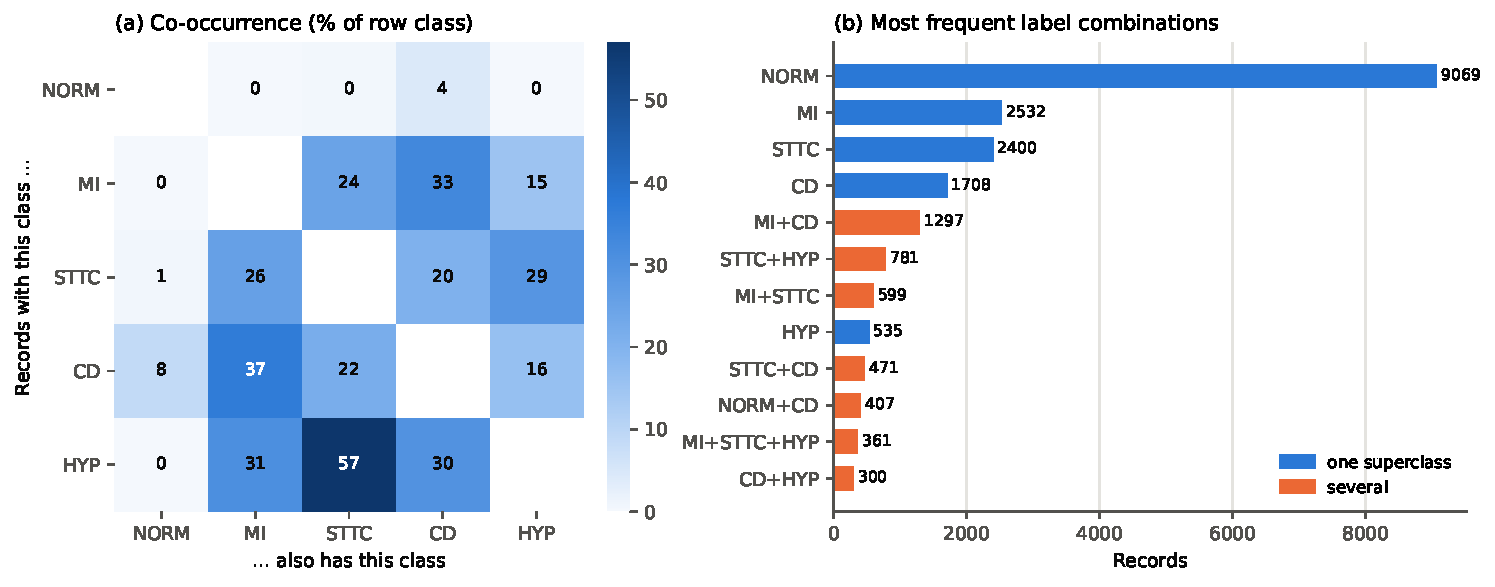
\includegraphics[width=\textwidth,height=0.42\textheight,keepaspectratio]{figures/eda_label_cooccurrence.pdf}
\caption[Co-occurrence and combinations of superclasses]{Multi-label structure. (a) Co-occurrence: percentage of the records of the row class that also carry the column class (not symmetric). (b) Most frequent label combinations; blue: one superclass, orange: several.}
\label{fig:eda_label_cooccurrence}
\end{figure}


The analysis found \edaNNanValuesTrain{} missing values and \edaNFlatLeadsTrain{} constant lead in the
training set (a lead whose metadata already notes an electrode problem); nothing was excluded. Its
conclusions for the design (records without a superclass left out, macro AUROC, sigmoid outputs,
patient-wise bootstrap, per-lead z-score) are discussed in the PRDL-DL report.

% =====================================================================
% 3. Training loop (T8, OF + MM) and evaluation module (T7, MM)
% =====================================================================
\section{Training and evaluation code}\label{sec:training}

\subsection{A task-agnostic training loop}

The loop (\texttt{src/train.py}, written by both of us) serves every classifier and the generators,
because everything specific to a task comes from a \emph{task} object: the loss, the metrics
(accumulated batch by batch, so that a generator never keeps all its logits in memory) and the
selection metric with its direction (macro AUROC, higher is better; or cross-entropy, lower is
better). Listing~\ref{lst:loop} shows the five steps of an epoch and the evaluation pass.

\lstinputlisting[firstnumber=101,caption={The training epoch and the evaluation pass
(\texttt{src/train.py}, lines 101--139).},label={lst:loop}]{common/code/train_one_epoch.py}

PyTorch details behind these lines:
\begin{itemize}[leftmargin=1.2em,itemsep=1pt]
  \item \texttt{optimizer.zero\_grad()} is needed because PyTorch \emph{adds} new gradients to the
        stored ones; \texttt{loss.backward()} fills \texttt{.grad} of every trainable parameter and
        \texttt{optimizer.step()} uses them.
  \item \texttt{model.train()} and \texttt{model.eval()} switch dropout and batch norm between their two
        behaviours; \texttt{@torch.no\_grad()} on the evaluation pass avoids building the autograd graph
        (less memory, faster).
  \item \texttt{loss.item()} turns the loss into a Python number, so the graph of the batch is not kept
        alive by the running sum. The evaluation sums the loss and divides once at the end, which gives
        the exact mean even if the last batch is smaller.
  \item The optimiser receives only parameters with \texttt{requires\_grad=True}; a frozen backbone
        (Section~\ref{sec:strategies-code}) therefore needs no special code. The run log records total and
        trainable parameters.
  \item Gradient clipping (\texttt{clip\_grad\_norm\_}) rescales the whole gradient when its norm exceeds
        a threshold; it is off for the Dense and CNN blocks and on for the others.
\end{itemize}

The classification loss is a single call (Listing~\ref{lst:bce}); the model outputs logits and the
sigmoid lives inside the loss.

\lstinputlisting[firstnumber=91,caption={Multi-label loss (\texttt{src/tasks.py}, lines 91--95). Class
weights are available but were not used.},label={lst:bce}]{common/code/multilabel_loss.py}

\subsection{Evaluation module (Mar\'ia's block, summary)}

\texttt{src/metrics.py} (task T7, done by Mar\'ia and reviewed by me) computes the AUROC per class with
scikit-learn, the macro AUROC as their plain mean, and per-class F1 thresholds chosen on validation on a
grid from 0.01 to 0.99. Intervals use the patient bootstrap of Listing~\ref{lst:boot}: each resample
draws patients with replacement and repeats every record of a drawn patient as many times as the
patient was drawn. Because the resamples depend only on the patients and the seed, two models
evaluated on the same split get the same resamples, which is what makes the paired comparison possible:
the difference of the two metrics is computed on each resample, and its percentiles give the interval
of the difference. Resamples in which a class has no positive or no negative record are discarded and
counted.

\lstinputlisting[firstnumber=101,caption={Patient bootstrap (\texttt{src/metrics.py}, lines
101--119).},label={lst:boot}]{common/code/patient_bootstrap.py}

\subsection{Run logs and numbers}

Every run writes \texttt{results/logs/<run\_id>.json} with its configuration, data description, model
size, per-epoch curves, best epoch, results per split, paths of the checkpoint and the saved predictions,
and \texttt{meta} (date, commit, whether the code under \texttt{src/} had uncommitted changes,
package versions, device). Each block summarises its runs in one summary log.
\texttt{report/runs.json} maps a short alias to each summary, and \texttt{report/make\_numbers.py}
turns every scalar of those logs into a \LaTeX{} macro (\texttt{\textbackslash cnnFinalTestMacroAurocMean}
expands to \cnnFinalTestMacroAurocMean{}). Only the files listed in \texttt{runs.json} are read, so an
old or smoke run cannot slip into a report, and a name collision stops the script. All the tables of the
blocks are generated from the summaries and contain only macros. These reports therefore contain no
measured number typed by hand; regenerating the logs and \texttt{numbers.tex} updates every report.

The flag for uncommitted code had a bug that the assistant first explained wrongly
(Appendix~\ref{app:ai-code}, Sheet C4): each run wrote its own predictions file before checking
\texttt{git status}, so every run looked ``dirty''. The check now looks only at the code under
\texttt{src/}.

% =====================================================================
% 4. Area 1 in code: Dense and CNN (own), RNN and Transformer (MM, summary)
% =====================================================================
\section{Area 1: core architectures in PyTorch}\label{sec:arch-code}

Each block has a model file in \texttt{src/models/}, registered by name so that
\texttt{python -m src.train --model <name>} can build it, an experiment script
(\texttt{src/<block>\_experiments.py} with \texttt{run}, \texttt{final} and \texttt{report}) and a test
file. The theory and the analysis of the results are in the PRDL-DL report; this section is about the
implementation and the training behaviour.

\subsection{Dense network (own block)}

\lstinputlisting[firstnumber=34,caption={Hidden blocks of \texttt{DenseNet} (\texttt{src/models/dense.py},
lines 34--51).},label={lst:dense}]{common/code/dense_net.py}

\begin{itemize}[leftmargin=1.2em,itemsep=1pt]
  \item \textbf{Flatten order.} \texttt{nn.Flatten} on $(B, 12, 1000)$ puts the 1000 samples of lead I
        first, then lead II, etc.; reshaping the first-layer weight to (units, 12, 1000) gives back one
        pattern per lead, which is how Figure~\ref{fig:dense_first_layer} was drawn.
  \item \textbf{The training loss is measured in training mode}, with dropout active, so it is higher
        than the loss of the same weights in evaluation mode; this is why in the first epochs the
        training curve can lie above the validation curve (Figure~\ref{fig:dense_curves}).
  \item \textbf{Batch norm in evaluation} uses running averages collected in training; forgetting
        \texttt{model.eval()} would make a prediction depend on the other records of the batch.
        \texttt{BatchNorm1d} also refuses a training batch of one record, a case we checked could not
        occur with our split sizes.
  \item \textbf{Cost.} One epoch takes \denseEpochTimeMeanBase{}\,s for the baseline; the network has
        \denseParamsBase{} parameters, almost all in the first Linear layer.
\end{itemize}

% Shared float (common/make_floats.py). Figure: figures/dense_curves.pdf
\begin{figure}[htbp]
\centering
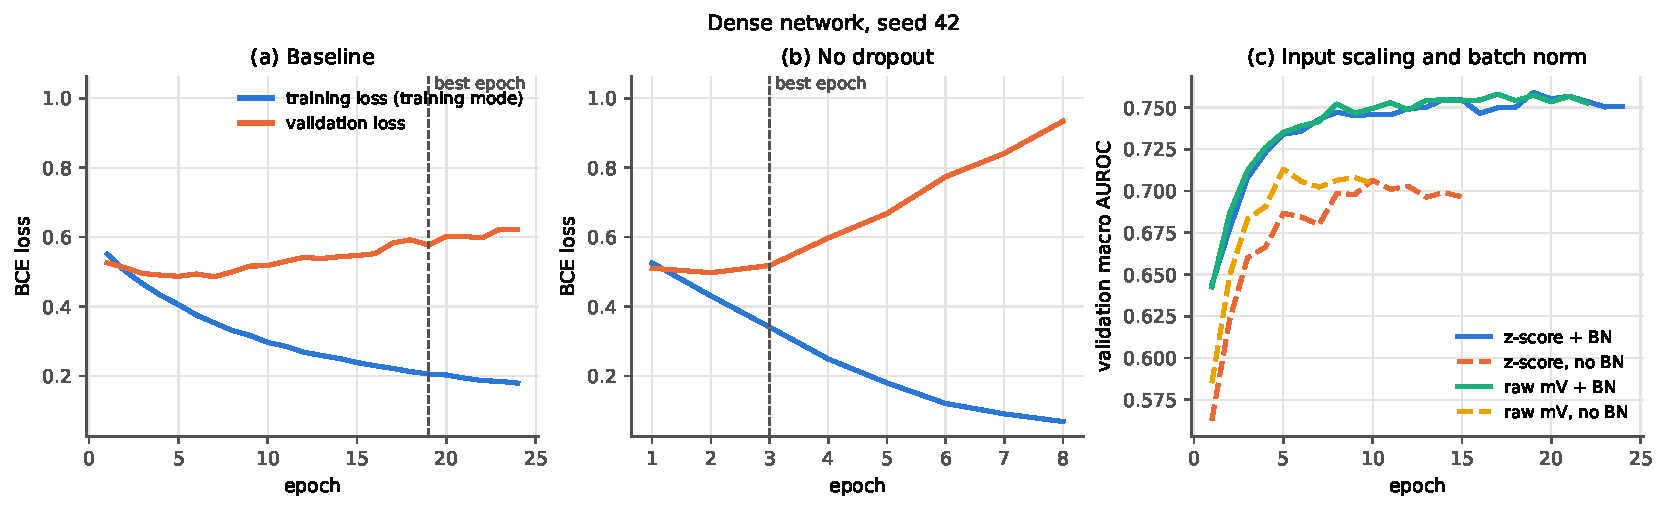
\includegraphics[width=\textwidth,height=0.42\textheight,keepaspectratio]{figures/dense_curves.pdf}
\caption[Dense network: learning curves]{Dense network, seed 42. (a) Baseline: training loss (measured in training mode, with dropout) and validation loss; dashed line: best epoch by validation macro AUROC. (b) The same without dropout. (c) Validation macro AUROC with and without input z-score and batch norm.}
\label{fig:dense_curves}
\end{figure}

% Shared float (common/make_floats.py). Figure: figures/dense_first_layer.pdf
\begin{figure}[htbp]
\centering
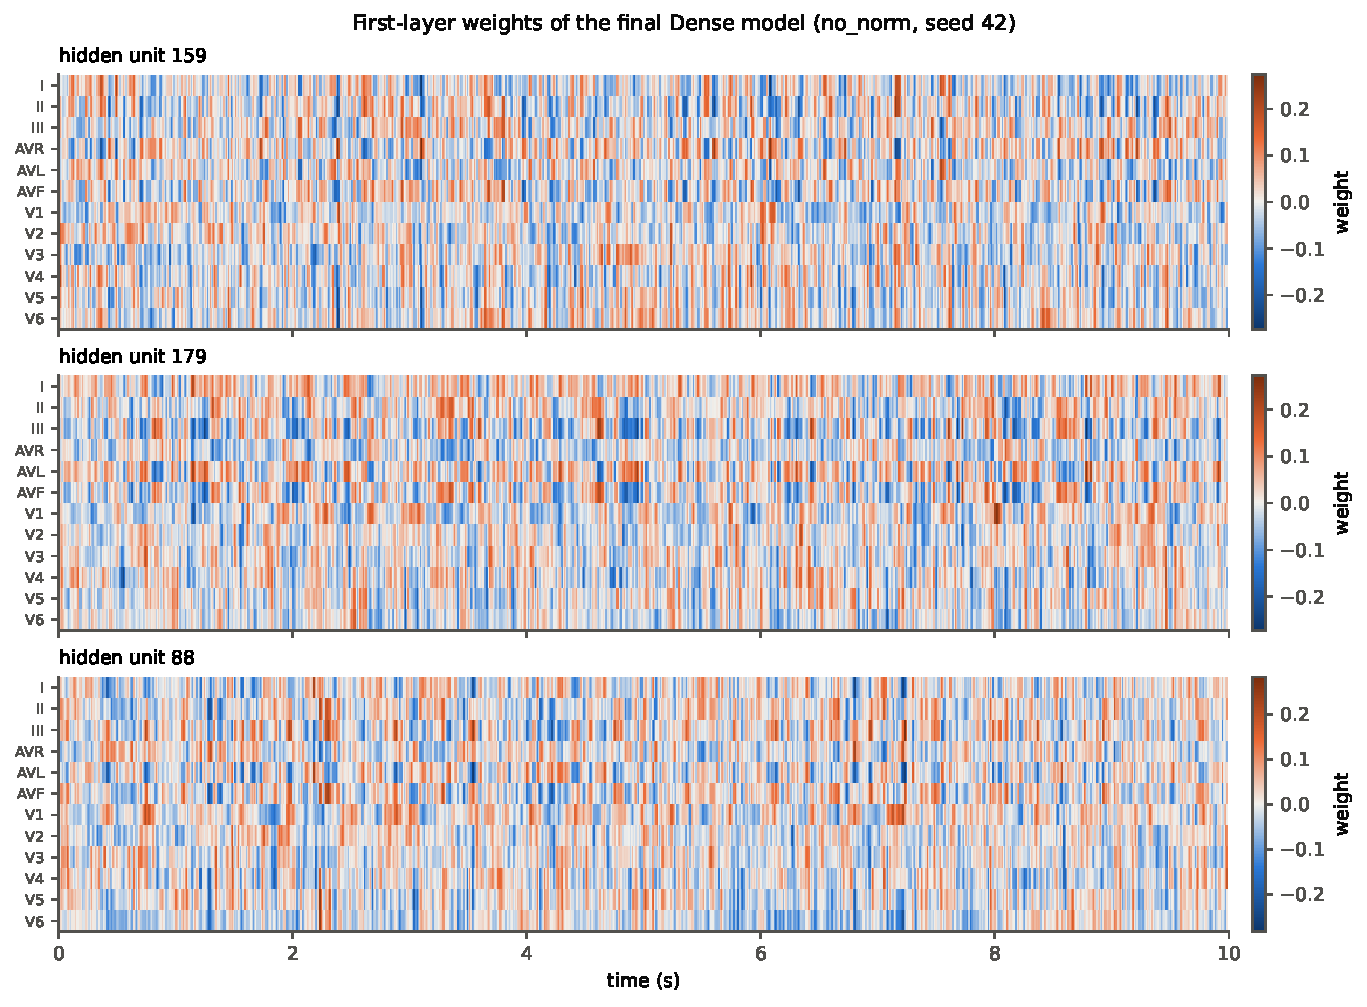
\includegraphics[width=\textwidth,height=0.42\textheight,keepaspectratio]{figures/dense_first_layer.pdf}
\caption[Dense network: first-layer weights]{First-layer weights of the final Dense model (\texttt{no\_norm}, seed 42) for the three hidden units with the largest weight norm, reshaped to 12 leads $\times$ 1000 samples.}
\label{fig:dense_first_layer}
\end{figure}


\subsection{1D CNN (own block)}

\lstinputlisting[firstnumber=31,caption={Residual block of the CNN (\texttt{src/models/cnn.py}, lines
31--70).},label={lst:conv}]{common/code/conv_block.py}

\begin{itemize}[leftmargin=1.2em,itemsep=1pt]
  \item \textbf{Layout.} \texttt{Conv1d} expects $(B, \text{channels}, \text{time})$; the cache already
        stores $(12, 1000)$, so no \texttt{permute} is needed. A $(B, \text{time}, \text{channels})$
        tensor would silently treat the 1000 samples as channels.
  \item \textbf{``Same'' padding needs an odd kernel.} \texttt{padding = k // 2} keeps the length only
        for odd $k$; the model refuses even kernels because the main path and the shortcut must have the
        same length to be added.
  \item \textbf{The skip connection is a plain \texttt{+}} (line 69). The identity shortcut adds no
        parameter, a $1\times1$ convolution adapts the number of channels where it changes, and autograd
        sends the gradient through both branches.
  \item \textbf{Receptive field.} \texttt{CNN1D.receptive\_field()} computes it from kernels and pooling;
        a test checks it against the gradient of a linearised copy of the network.
  \item \textbf{Interpretation.} Feature maps are read with forward hooks
        (\texttt{register\_forward\_hook}), removed in a \texttt{finally} block. With global average
        pooling and one Linear layer, the logit equals the bias plus the mean over time of the class
        activation map, in evaluation mode (in training mode dropout breaks the identity); a test checks
        it numerically.
  \item \textbf{Cost.} \cnnEpochTimeMeanBase{}\,s per epoch for the baseline, against
        \denseEpochTimeMeanBase{}\,s for the Dense network, with \cnnParamsBase{} parameters.
\end{itemize}

% Shared float (common/make_floats.py). Figure: figures/cnn_curves.pdf
\begin{figure}[htbp]
\centering
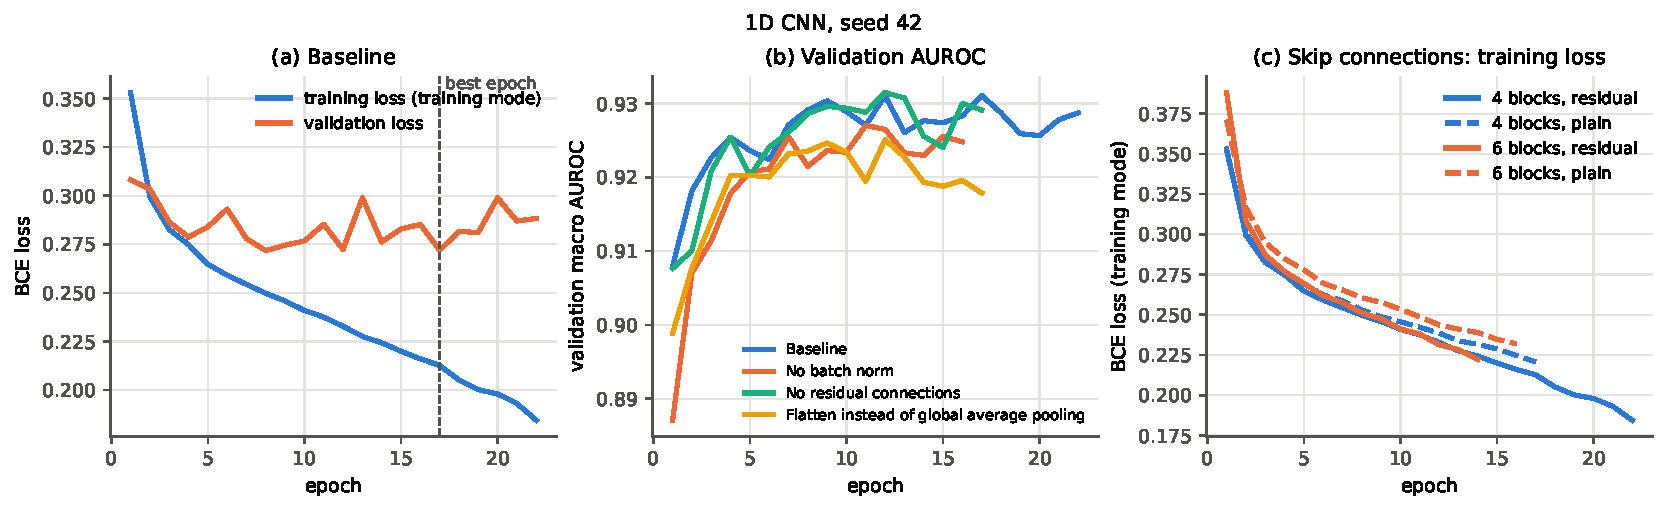
\includegraphics[width=\textwidth,height=0.42\textheight,keepaspectratio]{figures/cnn_curves.pdf}
\caption[1D CNN: learning curves]{1D CNN, seed 42. (a) Baseline training and validation loss; dashed line: best epoch. (b) Validation macro AUROC without batch norm, without residual connections and with flatten instead of global average pooling. (c) Training loss with and without residual connections, at 4 and 6 blocks.}
\label{fig:cnn_curves}
\end{figure}


\subsection{Recurrent networks and Transformer (Mar\'ia's blocks, summary)}

\begin{itemize}[leftmargin=1.2em,itemsep=1pt]
  \item \textbf{Sequence layout.} The record $(B, 12, 1000)$ becomes a sequence $(B, T, \text{features})$
        with \texttt{batch\_first=True}, the opposite axis order of \texttt{Conv1d}: 100 frames of
        10 samples (120 numbers per step), 1000 raw steps, or the 125 steps of a convolutional front end
        that reuses the CNN's \texttt{ConvBlock}.
  \item \textbf{Readouts.} The last state is \texttt{h\_n[-1]} (last layer); mean pooling averages
        \texttt{out} over time; attention pooling scores each state, applies a softmax over time and
        takes the weighted sum.
  \item \textbf{Stability and determinism.} Gradient clipping at norm 1 in every configuration, and
        \texttt{CUBLAS\_WORKSPACE\_CONFIG} so that the GPU runs of \texttt{nn.LSTM} are reproducible.
  \item \textbf{Hand-written attention.} \texttt{src/models/attention.py} implements scaled dot-product
        attention, multi-head attention and a Pre-LN/Post-LN Transformer block as in the course
        notebooks, with an optional causal mask (Listing~\ref{lst:causal}); a test checks it against
        \texttt{nn.MultiheadAttention} with the same weights, with and without the mask. Patches are
        embedded by a Linear layer, which a test shows to be a \texttt{Conv1d} with kernel and stride 10.
  \item \textbf{Cost.} The 1000-step LSTM is the slowest classifier (\rnnEpochTimeMeanRaw{}\,s per
        epoch against \rnnEpochTimeMeanBase{}\,s with 100 frames) and needs many more epochs, the
        difficulty of backpropagation through many time steps; the Transformer baseline takes
        \transformerEpochTimeMeanBase{}\,s.
\end{itemize}

% Shared float (common/make_floats.py). Figure: figures/rnn_curves.pdf
\begin{figure}[htbp]
\centering
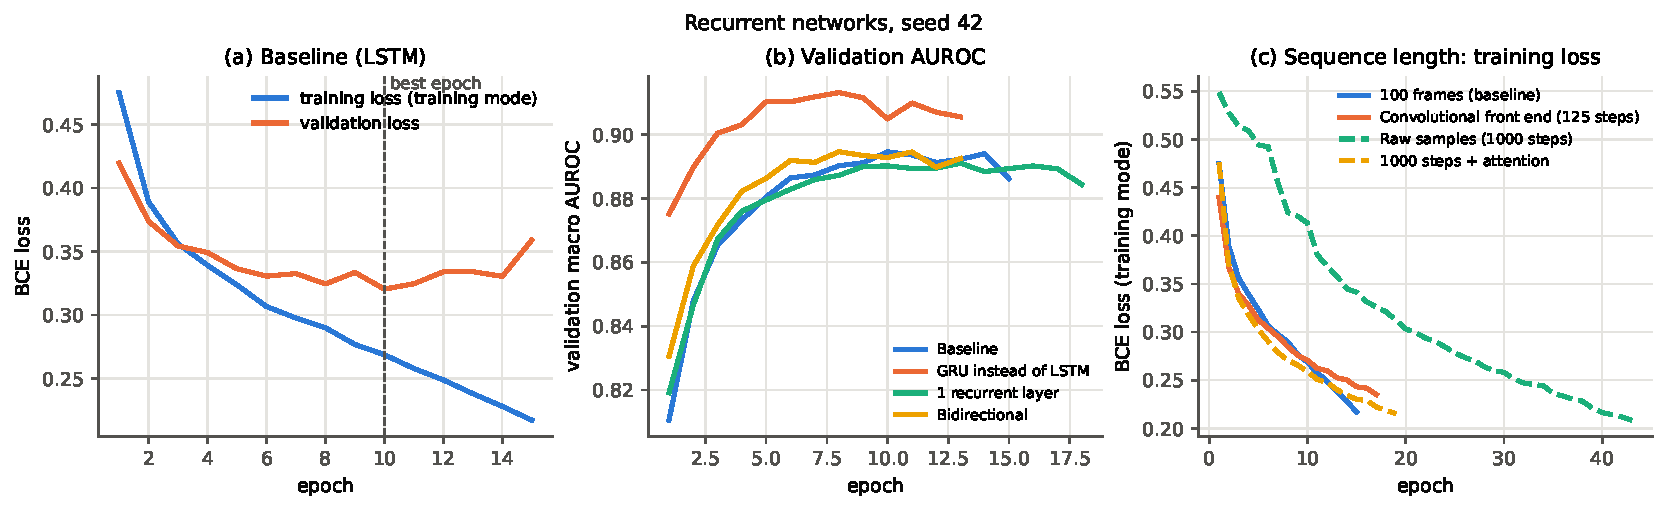
\includegraphics[width=\textwidth,height=0.42\textheight,keepaspectratio]{figures/rnn_curves.pdf}
\caption[Recurrent networks: learning curves]{Recurrent networks, seed 42. (a) LSTM baseline losses. (b) Validation macro AUROC of the baseline, GRU, one recurrent layer and bidirectional LSTM. (c) Training loss with 100 frames, the convolutional front end, 1000 raw steps and 1000 steps with attention.}
\label{fig:rnn_curves}
\end{figure}


Test results of every family are in Table~\ref{tab:comparison_final} (Section~\ref{sec:code}).
In the Dense and CNN blocks the validation loss reaches its minimum earlier than the validation AUROC,
so early stopping on the AUROC lets the models train past the loss minimum: the ranking of the records
keeps improving while the probabilities become over-confident.

% =====================================================================
% 5. Area 2 in code: transfer from the ECG-GPT and zero-shot CLIP
%    (T13, T24: shared tasks, OF + MM)
% =====================================================================
\section{Area 2: learning strategies in code}\label{sec:strategies-code}

\subsection{Transfer from the ECG-GPT}

The pre-trained model is the generator of area 3 selected by the rule of that block (lowest validation
bits per sample), fixed before any transfer run: the ECG-GPT with one token per microvolt. Its summary
log hands over the model arguments, the checkpoints of the three seeds and the tokenizer; the transfer
run with seed $s$ loads the generator pre-trained with seed $s$, so the three seeds are three independent
pre-training + transfer pairs. Listing~\ref{lst:transfer} shows the classifier used by the three
strategies.

\lstinputlisting[firstnumber=185,caption={Generator backbone + new head (\texttt{src/transfer.py}, lines
185--212).},label={lst:transfer}]{common/code/transfer_classifier.py}

\begin{itemize}[leftmargin=1.2em,itemsep=1pt]
  \item \textbf{Loading.} The checkpoint is a \texttt{state\_dict}; it is loaded into a freshly built
        generator and the next-token head is discarded. \texttt{record\_features} averages the outputs of
        the final LayerNorm over the four windows of 250 samples that cover a record.
  \item \textbf{Freezing.} The linear probe sets \texttt{requires\_grad=False} on the backbone, and
        \texttt{train()} is overridden so that the backbone stays in evaluation mode even when the loop
        calls \texttt{model.train()}: its dropout is off and a record always gives the same vector, as a
        fixed feature extractor should.
  \item \textbf{A faster probe.} Because the frozen vectors never change, they are computed once per
        checkpoint and the head (\texttt{FeatureHead}) is trained on them; a test checks that this gives
        exactly the output of the frozen full model. A probe epoch takes
        \transferEpochTimeMedianProbeFOneZeroZero{}\,s against \transferEpochTimeMedianFinetuneFOneZeroZero{}\,s
        for fine-tuning with all the labels.
  \item \textbf{Learning rates.} $10^{-3}$ for the head and for training from scratch; $10^{-4}$ for
        fine-tuning, as in the optional fine-tuning cell of the course notebook \cite{course_nb_transfer}.
        Two ablations (fine-tuning at $10^{-3}$, scratch at $10^{-4}$) separate the effect of the
        pre-trained weights from that of the rate.
  \item \textbf{Memory.} One record is four windows of 250 tokens; the activations kept for
        backpropagation of 32 records already take about a gigabyte (measured on the CPU before the runs),
        so the transfer experiments use batches of 32 records instead of 64 on the 4\,GB GPU, the same for
        every configuration.
  \item \textbf{10\,\% of the labels, drawn by patient.} Training patients are shuffled with the run's
        seed and taken with all their records until 10\,\% of the training records is reached; the subset
        is the same for the three strategies of a seed (paired comparison) and its class counts are logged.
\end{itemize}

% Shared float (common/make_floats.py). Figure: figures/transfer_curves.pdf
\begin{figure}[htbp]
\centering
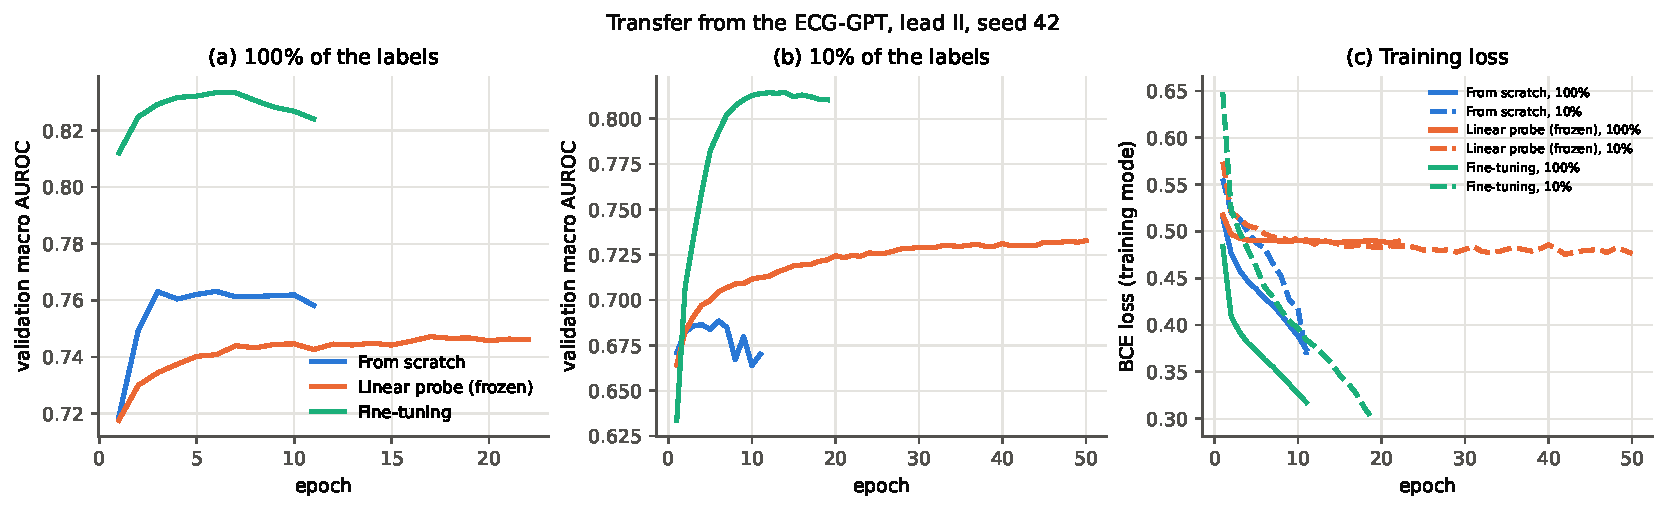
\includegraphics[width=\textwidth,height=0.42\textheight,keepaspectratio]{figures/transfer_curves.pdf}
\caption[Transfer from the ECG-GPT: learning curves]{Transfer from the ECG-GPT, lead II, seed 42: validation macro AUROC with (a) 100\,\% and (b) 10\,\% of the training labels, and (c) training loss of the three strategies.}
\label{fig:transfer_curves}
\end{figure}


The curves (Figure~\ref{fig:transfer_curves}) show what the numbers in the PRDL-DL report summarise:
fine-tuning starts high and peaks within a few epochs, training from scratch reaches its best epoch early (on average
\intval{\transferBestEpochMeanScratchFOneZeroZero} with all labels) and then overfits, and the probe with 10\,\% of the labels was still rising slowly near the 50-epoch limit (best
epoch \intval{\transferBestEpochMeanProbeFOneZero} on average): it was limited by the budget.

\subsection{Zero-shot with CLIP}

\begin{itemize}[leftmargin=1.2em,itemsep=1pt]
  \item \textbf{Model.} CLIP ViT-B/32 with OpenAI's weights, the model of the course notebook
        \cite{course_nb_clip}, loaded with \texttt{open\_clip}. The first run warned that open\_clip's plain
        \texttt{ViT-B-32} uses GELU while these weights were trained with QuickGELU, so the model is loaded
        as \texttt{ViT-B-32-quickgelu}. Nothing is trained or tuned.
  \item \textbf{Where zero-shot should work.} CIFAR-100 test images with the notebook's prompt and with the
        bare label; top-1 and top-5 accuracy with a bootstrap interval over images.
  \item \textbf{ECG as images.} Lead II of every validation and test record drawn as a $224\times224$
        image (two rows of 5\,s on a light grid, fixed scale), the size CLIP expects, so its preprocessing
        does not crop. One fixed sentence per superclass; class scores are the softmax over the five
        sentences of the scaled cosine similarity, as in the notebook. A modality check compares
        ``an electrocardiogram'' with five unrelated sentences.
  \item \textbf{A device bug} stopped the first run: image embeddings were moved to the CPU and text
        embeddings stayed on the GPU (documented in Mar\'ia's MLLB report, Sheet C3; error B10 of the AI log).
\end{itemize}

% Shared float (common/make_floats.py). Figure: figures/zeroshot_ptbxl.pdf
\begin{figure}[htbp]
\centering
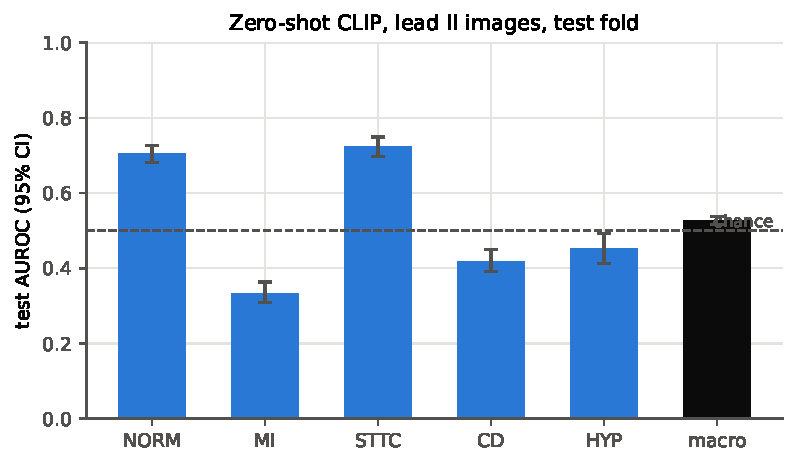
\includegraphics[width=\textwidth,height=0.42\textheight,keepaspectratio]{figures/zeroshot_ptbxl.pdf}
\caption[Zero-shot CLIP on PTB-XL]{Zero-shot CLIP on the test fold: AUROC per superclass and macro AUROC with 95\,\% patient-bootstrap intervals; dashed line: chance.}
\label{fig:zeroshot_ptbxl}
\end{figure}


\subsection{Twelve leads against lead II}

Every model class accepts \texttt{n\_leads=1}. The final model of each family was trained again on lead
II with everything else copied from its 12-lead final runs, as \texttt{--final} runs named
\texttt{onelead\_<family>\_...}, so they never mix with the 12-lead runs that each block's summary reads.
Results are in Table~\ref{tab:comparison_final}.

% =====================================================================
% 6. Area 3 in code: ECG-GPT and LSTM generators (T23, own block)
% =====================================================================
\section{Area 3: autoregressive generators in code (own block)}\label{sec:generative-code}

\subsection{From signal to tokens}

PTB-XL stores every sample as an integer number of microvolts (the code checks it on the training data:
a share \generativeFracOffUvGridTrain{} of the values is off the grid), so the tokenizer
(Listing~\ref{lst:tok}) is exact inside its range. A value in millivolts becomes an integer number of
microvolts, its token is the floor division by the level width $\Delta$ after subtracting the lower end of
the range, and values outside go to the first or last token. The range is 2.56\,mV wide, from
\generativeRangeLoUv{} to \generativeRangeHiUv{}\,\textmu V, centred on training quantiles of lead II.

\lstinputlisting[firstnumber=69,caption={Tokenizer on the microvolt grid (\texttt{src/generative.py},
lines 69--74).},label={lst:tok}]{common/code/tokenizer.py}

Training items are windows of $L+1$ samples starting at a random position of a training record: the
first $L$ tokens are the input and the same tokens shifted by one are the target (teacher forcing). The
window start is drawn from a NumPy generator seeded with the run's seed, which is reproducible because
data loading runs in the main process. An epoch shows every training record once through one random
window. Validation uses fixed windows that together cover every target of every record.

\subsection{Model and loss}

The ECG-GPT reuses Mar\'ia's Transformer blocks with \texttt{causal=True}. The mask is a lower-triangular
boolean matrix, and masked scores are set to $-\infty$ before the softmax, so their weights are exactly
zero (Listing~\ref{lst:causal}; a test checks that the attention maps are lower-triangular and that
changing a future token does not change past outputs).

\lstinputlisting[firstnumber=29,caption={Causal mask and scaled dot-product attention
(\texttt{src/models/attention.py}, lines 29--62).},label={lst:causal}]{common/code/causal_attention.py}

\begin{itemize}[leftmargin=1.2em,itemsep=1pt]
  \item \textbf{Embeddings.} \texttt{nn.Embedding(V, 128)} gives one learned vector per level, as one
        vector per character in the course's text-generation notebooks. The sinusoidal positional encoding
        is a non-persistent buffer: it moves to the GPU with the model, is not trained and is not stored in
        the checkpoint.
  \item \textbf{Cross-entropy over sequences.} Logits $(B, T, V)$ are reshaped to $(B\cdot T, V)$ and
        targets to $(B\cdot T)$ before \texttt{F.cross\_entropy}; otherwise PyTorch would read $T$ as the
        class axis. No softmax in the model: the loss contains it.
  \item \textbf{Per-position cost.} \texttt{log\_softmax} followed by \texttt{gather} gives the
        cross-entropy of every position separately, which the mean loss hides; it is the curve of
        prediction cost against context shown in the PRDL-DL report.
  \item \textbf{Same size for a fair comparison.} The LSTM's hidden size was chosen so that it has about
        the same number of parameters as the ECG-GPT (\generativeParamsLstm{} against
        \generativeParamsBase{}).
\end{itemize}

\subsection{Generation}

Generation slides a window of $L$ tokens one sample at a time: the model predicts the next token from
the last $L$, the token is appended and the window moves. Both models use the same sliding window (the
LSTM state is not carried beyond $L$ samples, which it never saw in training). Only the last position
goes through the output layer. Listing~\ref{lst:sample} shows the sampling rule, following the course
notebook \cite{course_nb_sampling}.

\lstinputlisting[firstnumber=468,caption={Greedy, temperature and top-$k$ sampling
(\texttt{src/generative.py}, lines 468--485).},label={lst:sample}]{common/code/sample_next.py}

\begin{itemize}[leftmargin=1.2em,itemsep=1pt]
  \item \textbf{Reproducible sampling.} \texttt{torch.multinomial} draws with a \texttt{torch.Generator}
        seeded once per model, under \texttt{model.eval()} and \texttt{torch.no\_grad()}.
  \item \textbf{Memory grows with $L^2$.} Generating 64 windows of 500 tokens ran out of memory on the
        4\,GB GPU (Appendix~\ref{app:ai-code}, Sheet C1); generation batches now shrink as $(250/L)^2$ for
        longer contexts and the GPU is freed between models.
  \item \textbf{Cost.} The median epoch takes \generativeEpochTimeMedianBase{}\,s for the ECG-GPT
        baseline, \generativeEpochTimeMedianLstm{}\,s for the LSTM and \generativeEpochTimeMedianCtxFiveZeroZero{}\,s
        with a 5\,s context; the 24 runs took several hours of training, and almost all of them used the
        whole 50-epoch budget.
\end{itemize}

% Shared float (common/make_floats.py). Figure: figures/generative_curves.pdf
\begin{figure}[htbp]
\centering
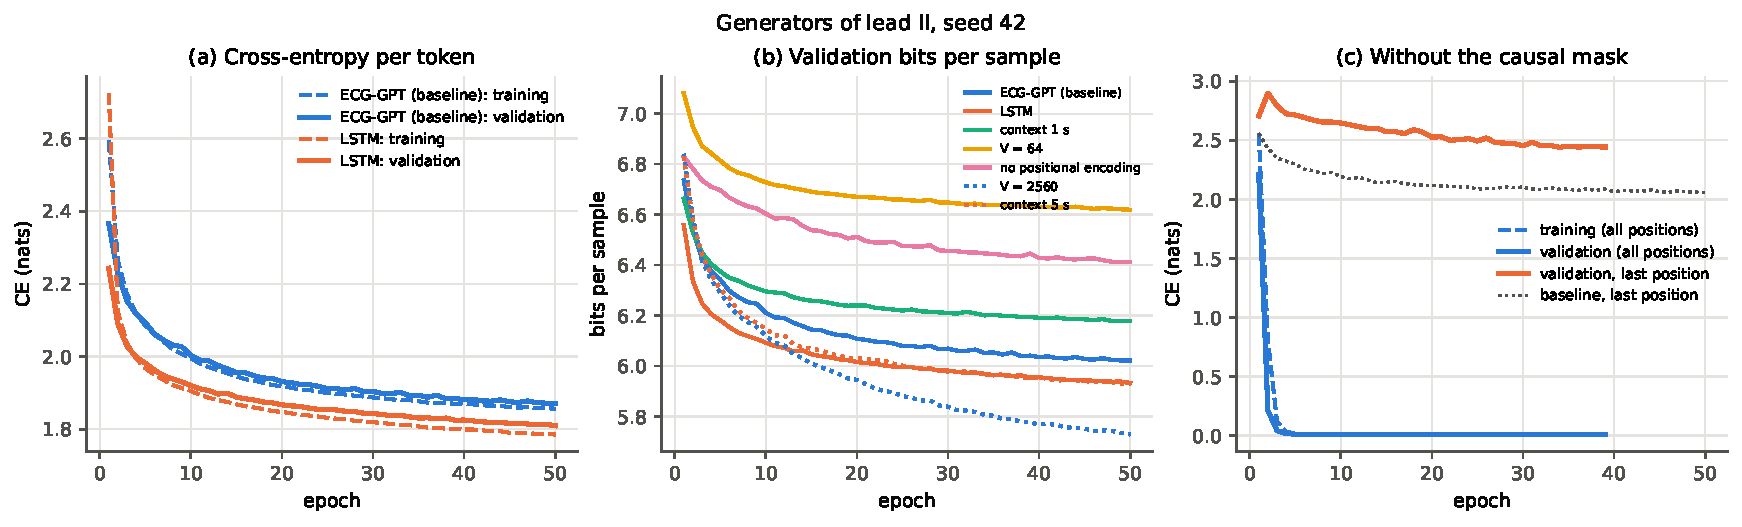
\includegraphics[width=\textwidth,height=0.42\textheight,keepaspectratio]{figures/generative_curves.pdf}
\caption[Generators: learning curves]{Generators of lead II, seed 42. (a) Cross-entropy per token of the ECG-GPT baseline and the LSTM. (b) Validation bits per sample of every configuration. (c) The ECG-GPT without the causal mask: training and validation cross-entropy over all positions and at the last position, with the baseline's last position for reference.}
\label{fig:generative_curves}
\end{figure}

% Shared float (common/make_floats.py). Figure: figures/generative_sampling.pdf
\begin{figure}[htbp]
\centering
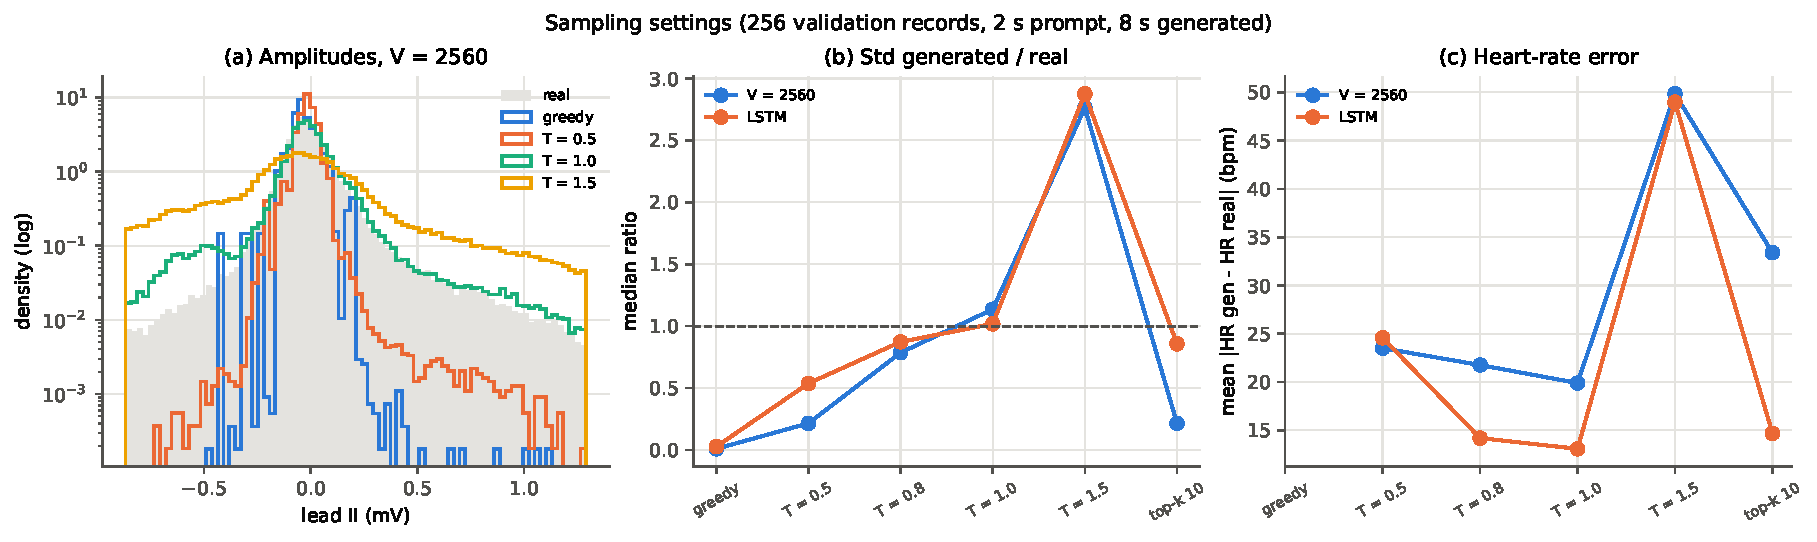
\includegraphics[width=\textwidth,height=0.42\textheight,keepaspectratio]{figures/generative_sampling.pdf}
\caption[Generators: sampling settings]{Sampling settings (256 validation records, 2\,s prompt, 8\,s generated). (a) Amplitude distributions of the generated signals against the real ones ($V = 2560$). (b) Median ratio of generated to real standard deviation. (c) Mean absolute heart-rate error.}
\label{fig:generative_sampling}
\end{figure}


\subsection{Evaluation code}

Besides cross-entropy and perplexity (exponential of the mean cross-entropy per token over the whole
split, not averaged per batch), the block computes bits per sample, unigram and bigram counting
baselines with add-one smoothing for each vocabulary, the ``next sample = this sample'' error, and, for
generated signals, the standard-deviation ratio, the share of flat records, the Wasserstein distance
between amplitude distributions and a heart rate from R peaks (local maxima above a threshold taken
from the real prompt, at least 0.3\,s apart). The heart-rate rule is simple and not a validated
detector; it finds a rate in a share \generativeRealHrDefinedFrac{} of the real continuations.

% =====================================================================
% 7. Code distribution and reproduction
% =====================================================================
\section{Code distribution and reproduction}\label{sec:code}

\subsection{Repository}

All code, run logs, figures, tables and the sources of the four reports are in the public repository
\url{https://github.com/orianafe16/ptbxl-DL}:

\begin{lstlisting}[language={},numbers=none,caption={Structure of the repository.},label={lst:tree}]
src/          data, models (src/models/), training loop, metrics, one *_experiments.py per block
tests/        pytest suite, one file per block (synthetic data; the real cache when present)
notebooks/    EDA and zero-shot notebooks (they call the functions of src/)
results/logs/ one JSON per run and one summary per block (checkpoints and caches not committed)
report/       numbers.tex (generated), runs.json, published.json, tables/, figures/,
              common/ (shared LaTeX), one main file per report
docs/         DECISIONS.md, PLAN_DL.md, AI_USAGE_LOG.md, blocks/ (one note per block),
              literature/ (prompts, checked quotes, learning-strategies material)
\end{lstlisting}

The data are not committed: the README explains how to download PTB-XL 1.0.3 from PhysioNet, and
\texttt{python -m src.prepare\_data} checks the files against the dataset's checksums and rebuilds the
cache. Checkpoints and smoke-run outputs are ignored by git.

\subsection{Reproducing the results}

On a Windows laptop with an NVIDIA GPU (the README also covers the CPU case):
\begin{lstlisting}[language={},numbers=none,caption={Commands to reproduce the project, from the folder \texttt{ptbxl-dl}.},label={lst:repro}]
py -3.12 -m venv .venv ; .venv\Scripts\activate
pip install torch --index-url https://download.pytorch.org/whl/cu126
pip install -r requirements.txt
python -m src.check_env ; python -m pytest -q tests
python -m src.prepare_data                       # checksums + cache
python -m src.eda                                # EDA: eda.json and figures
python -m src.train --model trivial --final      # trivial reference
python -m src.dense_experiments all              # likewise cnn_, rnn_, transformer_
python -m src.generative_experiments all         # generators (no test fold)
python -m src.transfer_experiments run ; python -m src.transfer_experiments report
python -m src.leads_experiments all ; python -m src.zero_shot run
python -m src.comparison report                  # final table and figures
python report/make_numbers.py                    # report/numbers.tex
python report/common/make_floats.py              # shared figure/table floats
python report/common/make_contributions.py       # contribution tables from PLAN_DL.md
python report/common/make_code_excerpts.py       # code listings of this report
\end{lstlisting}

The order matters: each block compares its final models with those of earlier blocks (Dense, then CNN,
RNN and Transformer), the generators must exist before the transfer experiments, and the comparison comes
last. Every block also has a smoke mode (\texttt{all --fast}) and, where runs are long, an \texttt{estimate}
step. Reproduction has three levels. Without data or GPU, a clean clone runs the tests on synthetic data
and rebuilds \file{numbers.tex} from the committed logs (we checked that the macros come out identical),
which is all the reports need. With the data and the checkpoints (kept outside git and backed up
separately), the \texttt{report} steps rebuild every table and figure, including those that load a model.
Retraining repeats the runs, with small GPU differences because the fully deterministic mode of PyTorch is
not enabled. The reports compile from \texttt{report/} (on Overleaf, the folder \texttt{report/} uploaded as a
project with \texttt{oriana\_mllb.tex} as main file).

\subsection{Tests}

Each block has its tests, run before every long execution: data (shapes, no patient in two splits, class
counts against PhysioNet, normalisation statistics from training records only), metrics on toy cases,
the loop over-fitting a small batch, receptive field and class activation maps of the CNN, attention
against \texttt{nn.MultiheadAttention} with and without the causal mask, causality of the generators,
the tokenizer, the frozen backbone of the probe, and every pipeline end to end on synthetic data.
Regression tests were added for each code error found (Appendix~\ref{app:ai-code}).

\subsection{Final results and traceability}

% Shared float (common/make_floats.py). Table: tables/comparison_final.tex
\begin{table}[htbp]
\centering
\caption[Final comparison (test)]{Final comparison on the test fold. Mean $\pm$ SD over seeds; interval: 95\,\% patient bootstrap of the first seed. Published rows: macro AUC of the superclass task in Table~I of \cite{strodthoff2021deep}, obtained in a different setting (described in the text).}
\label{tab:comparison_final}
\small
\begin{adjustbox}{max width=\textwidth}
% Generated by src/comparison.py from results/logs/comparison_summary.json.
% Mean +- SD over seeds (one run: no SD); CI = 95% patient bootstrap of the first seed. Needs alias "comparison".
\begin{tabular}{lcrrccc}
\toprule
Model & Labels & Train.\ param. & Seeds & Test macro AUROC & First seed [95\% CI] & Test macro F1 \\
\midrule
\multicolumn{7}{l}{\textit{12 leads}} \\
\quad Trivial (lead mean and SD) & 100\% & \comparisonParamsTrivial{} & \comparisonNSeedsTrivial{} & \comparisonTestAurocMeanTrivial{} & \comparisonTestAurocFirstTrivial{} [\comparisonTestAurocLoFirstTrivial{}, \comparisonTestAurocHiFirstTrivial{}] & \comparisonTestFOneMeanTrivial{} \\
\quad Dense & 100\% & \comparisonParamsTwelveDense{} & \comparisonNSeedsTwelveDense{} & \comparisonTestAurocMeanTwelveDense{} $\pm$ \comparisonTestAurocSdTwelveDense{} & \comparisonTestAurocFirstTwelveDense{} [\comparisonTestAurocLoFirstTwelveDense{}, \comparisonTestAurocHiFirstTwelveDense{}] & \comparisonTestFOneMeanTwelveDense{} $\pm$ \comparisonTestFOneSdTwelveDense{} \\
\quad CNN & 100\% & \comparisonParamsTwelveCnn{} & \comparisonNSeedsTwelveCnn{} & \comparisonTestAurocMeanTwelveCnn{} $\pm$ \comparisonTestAurocSdTwelveCnn{} & \comparisonTestAurocFirstTwelveCnn{} [\comparisonTestAurocLoFirstTwelveCnn{}, \comparisonTestAurocHiFirstTwelveCnn{}] & \comparisonTestFOneMeanTwelveCnn{} $\pm$ \comparisonTestFOneSdTwelveCnn{} \\
\quad RNN & 100\% & \comparisonParamsTwelveRnn{} & \comparisonNSeedsTwelveRnn{} & \comparisonTestAurocMeanTwelveRnn{} $\pm$ \comparisonTestAurocSdTwelveRnn{} & \comparisonTestAurocFirstTwelveRnn{} [\comparisonTestAurocLoFirstTwelveRnn{}, \comparisonTestAurocHiFirstTwelveRnn{}] & \comparisonTestFOneMeanTwelveRnn{} $\pm$ \comparisonTestFOneSdTwelveRnn{} \\
\quad RNN + attention & 100\% & \comparisonParamsTwelveRnnattn{} & \comparisonNSeedsTwelveRnnattn{} & \comparisonTestAurocMeanTwelveRnnattn{} $\pm$ \comparisonTestAurocSdTwelveRnnattn{} & \comparisonTestAurocFirstTwelveRnnattn{} [\comparisonTestAurocLoFirstTwelveRnnattn{}, \comparisonTestAurocHiFirstTwelveRnnattn{}] & \comparisonTestFOneMeanTwelveRnnattn{} $\pm$ \comparisonTestFOneSdTwelveRnnattn{} \\
\quad Transformer & 100\% & \comparisonParamsTwelveTransformer{} & \comparisonNSeedsTwelveTransformer{} & \comparisonTestAurocMeanTwelveTransformer{} $\pm$ \comparisonTestAurocSdTwelveTransformer{} & \comparisonTestAurocFirstTwelveTransformer{} [\comparisonTestAurocLoFirstTwelveTransformer{}, \comparisonTestAurocHiFirstTwelveTransformer{}] & \comparisonTestFOneMeanTwelveTransformer{} $\pm$ \comparisonTestFOneSdTwelveTransformer{} \\
\addlinespace
\multicolumn{7}{l}{\textit{Lead II only (T14)}} \\
\quad Dense & 100\% & \comparisonParamsOneleadDense{} & \comparisonNSeedsOneleadDense{} & \comparisonTestAurocMeanOneleadDense{} $\pm$ \comparisonTestAurocSdOneleadDense{} & \comparisonTestAurocFirstOneleadDense{} [\comparisonTestAurocLoFirstOneleadDense{}, \comparisonTestAurocHiFirstOneleadDense{}] & \comparisonTestFOneMeanOneleadDense{} $\pm$ \comparisonTestFOneSdOneleadDense{} \\
\quad CNN & 100\% & \comparisonParamsOneleadCnn{} & \comparisonNSeedsOneleadCnn{} & \comparisonTestAurocMeanOneleadCnn{} $\pm$ \comparisonTestAurocSdOneleadCnn{} & \comparisonTestAurocFirstOneleadCnn{} [\comparisonTestAurocLoFirstOneleadCnn{}, \comparisonTestAurocHiFirstOneleadCnn{}] & \comparisonTestFOneMeanOneleadCnn{} $\pm$ \comparisonTestFOneSdOneleadCnn{} \\
\quad RNN & 100\% & \comparisonParamsOneleadRnn{} & \comparisonNSeedsOneleadRnn{} & \comparisonTestAurocMeanOneleadRnn{} $\pm$ \comparisonTestAurocSdOneleadRnn{} & \comparisonTestAurocFirstOneleadRnn{} [\comparisonTestAurocLoFirstOneleadRnn{}, \comparisonTestAurocHiFirstOneleadRnn{}] & \comparisonTestFOneMeanOneleadRnn{} $\pm$ \comparisonTestFOneSdOneleadRnn{} \\
\quad RNN + attention & 100\% & \comparisonParamsOneleadRnnattn{} & \comparisonNSeedsOneleadRnnattn{} & \comparisonTestAurocMeanOneleadRnnattn{} $\pm$ \comparisonTestAurocSdOneleadRnnattn{} & \comparisonTestAurocFirstOneleadRnnattn{} [\comparisonTestAurocLoFirstOneleadRnnattn{}, \comparisonTestAurocHiFirstOneleadRnnattn{}] & \comparisonTestFOneMeanOneleadRnnattn{} $\pm$ \comparisonTestFOneSdOneleadRnnattn{} \\
\quad Transformer & 100\% & \comparisonParamsOneleadTransformer{} & \comparisonNSeedsOneleadTransformer{} & \comparisonTestAurocMeanOneleadTransformer{} $\pm$ \comparisonTestAurocSdOneleadTransformer{} & \comparisonTestAurocFirstOneleadTransformer{} [\comparisonTestAurocLoFirstOneleadTransformer{}, \comparisonTestAurocHiFirstOneleadTransformer{}] & \comparisonTestFOneMeanOneleadTransformer{} $\pm$ \comparisonTestFOneSdOneleadTransformer{} \\
\addlinespace
\multicolumn{7}{l}{\textit{Lead II, ECG-GPT transfer (T13)}} \\
\quad ECG-GPT, from scratch & 100\% & \comparisonParamsScratchFOneZeroZero{} & \comparisonNSeedsScratchFOneZeroZero{} & \comparisonTestAurocMeanScratchFOneZeroZero{} $\pm$ \comparisonTestAurocSdScratchFOneZeroZero{} & \comparisonTestAurocFirstScratchFOneZeroZero{} [\comparisonTestAurocLoFirstScratchFOneZeroZero{}, \comparisonTestAurocHiFirstScratchFOneZeroZero{}] & \comparisonTestFOneMeanScratchFOneZeroZero{} $\pm$ \comparisonTestFOneSdScratchFOneZeroZero{} \\
\quad ECG-GPT, linear probe (frozen) & 100\% & \comparisonParamsProbeFOneZeroZero{} & \comparisonNSeedsProbeFOneZeroZero{} & \comparisonTestAurocMeanProbeFOneZeroZero{} $\pm$ \comparisonTestAurocSdProbeFOneZeroZero{} & \comparisonTestAurocFirstProbeFOneZeroZero{} [\comparisonTestAurocLoFirstProbeFOneZeroZero{}, \comparisonTestAurocHiFirstProbeFOneZeroZero{}] & \comparisonTestFOneMeanProbeFOneZeroZero{} $\pm$ \comparisonTestFOneSdProbeFOneZeroZero{} \\
\quad ECG-GPT, fine-tuning & 100\% & \comparisonParamsFinetuneFOneZeroZero{} & \comparisonNSeedsFinetuneFOneZeroZero{} & \comparisonTestAurocMeanFinetuneFOneZeroZero{} $\pm$ \comparisonTestAurocSdFinetuneFOneZeroZero{} & \comparisonTestAurocFirstFinetuneFOneZeroZero{} [\comparisonTestAurocLoFirstFinetuneFOneZeroZero{}, \comparisonTestAurocHiFirstFinetuneFOneZeroZero{}] & \comparisonTestFOneMeanFinetuneFOneZeroZero{} $\pm$ \comparisonTestFOneSdFinetuneFOneZeroZero{} \\
\quad ECG-GPT, from scratch & 10\% & \comparisonParamsScratchFOneZero{} & \comparisonNSeedsScratchFOneZero{} & \comparisonTestAurocMeanScratchFOneZero{} $\pm$ \comparisonTestAurocSdScratchFOneZero{} & \comparisonTestAurocFirstScratchFOneZero{} [\comparisonTestAurocLoFirstScratchFOneZero{}, \comparisonTestAurocHiFirstScratchFOneZero{}] & \comparisonTestFOneMeanScratchFOneZero{} $\pm$ \comparisonTestFOneSdScratchFOneZero{} \\
\quad ECG-GPT, linear probe (frozen) & 10\% & \comparisonParamsProbeFOneZero{} & \comparisonNSeedsProbeFOneZero{} & \comparisonTestAurocMeanProbeFOneZero{} $\pm$ \comparisonTestAurocSdProbeFOneZero{} & \comparisonTestAurocFirstProbeFOneZero{} [\comparisonTestAurocLoFirstProbeFOneZero{}, \comparisonTestAurocHiFirstProbeFOneZero{}] & \comparisonTestFOneMeanProbeFOneZero{} $\pm$ \comparisonTestFOneSdProbeFOneZero{} \\
\quad ECG-GPT, fine-tuning & 10\% & \comparisonParamsFinetuneFOneZero{} & \comparisonNSeedsFinetuneFOneZero{} & \comparisonTestAurocMeanFinetuneFOneZero{} $\pm$ \comparisonTestAurocSdFinetuneFOneZero{} & \comparisonTestAurocFirstFinetuneFOneZero{} [\comparisonTestAurocLoFirstFinetuneFOneZero{}, \comparisonTestAurocHiFirstFinetuneFOneZero{}] & \comparisonTestFOneMeanFinetuneFOneZero{} $\pm$ \comparisonTestFOneSdFinetuneFOneZero{} \\
\addlinespace
\multicolumn{7}{l}{\textit{Lead II, zero-shot (T24)}} \\
\quad CLIP ViT-B/32, zero-shot & 0\% & --- & \comparisonNSeedsZeroshot{} & \comparisonTestAurocMeanZeroshot{} & \comparisonTestAurocFirstZeroshot{} [\comparisonTestAurocLoFirstZeroshot{}, \comparisonTestAurocHiFirstZeroshot{}] & \comparisonTestFOneMeanZeroshot{} \\
\addlinespace
\multicolumn{7}{l}{\textit{Published (quoted, different settings: see text)}} \\
\quad resnet1d\_wang, 12 leads~\cite{strodthoff2021deep} & & & & \comparisonPublishedStrodthoffResnetOneDWang{} & & \\
\quad xresnet1d101, 12 leads~\cite{strodthoff2021deep} & & & & \comparisonPublishedStrodthoffXresnetOneDOneZeroOne{} & & \\
\quad lstm, 12 leads~\cite{strodthoff2021deep} & & & & \comparisonPublishedStrodthoffLstm{} & & \\
\quad fcn\_wang, 12 leads~\cite{strodthoff2021deep} & & & & \comparisonPublishedStrodthoffFcnWang{} & & \\
\quad inception1d, 12 leads~\cite{strodthoff2021deep} & & & & \comparisonPublishedStrodthoffInceptionOneD{} & & \\
\quad lstm\_bidir, 12 leads~\cite{strodthoff2021deep} & & & & \comparisonPublishedStrodthoffLstmBidir{} & & \\
\quad Wavelet+NN, 12 leads~\cite{strodthoff2021deep} & & & & \comparisonPublishedStrodthoffWaveletNn{} & & \\
\quad ensemble, 12 leads~\cite{strodthoff2021deep} & & & & \comparisonPublishedStrodthoffEnsemble{} & & \\
\bottomrule
\end{tabular}

\end{adjustbox}
\end{table}


Table~\ref{tab:comparison_final} collects every final model; each value is a macro whose source is the
summary log of its block, and each summary lists the run logs it read. The runs of the learning-strategy
block were made one commit before their code was committed (the logs say so); we checked on the laptop
that every file under \texttt{src/} was the delivered version and committed it unchanged.

% =====================================================================
% 8. Practical conclusions and own activities
% =====================================================================
\section{Practical conclusions and my activities}\label{sec:conclusions}

\subsection{Practical conclusions}

\begin{enumerate}[leftmargin=1.4em,itemsep=1pt]
  \item \textbf{A shared, task-agnostic loop paid off.} The same five-step loop, logging and comparison
        tools served five classifier families, two generators and the transfer experiments; differences
        between blocks are therefore differences between models, and a bug fixed once was fixed
        everywhere.
  \item \textbf{Smoke runs and estimates before long runs.} Every long grid was preceded by a
        \texttt{--fast} run and, where it existed, an \texttt{estimate}. The two failures on the real
        hardware happened in steps not covered by them (generation memory, CLIP on the GPU): what is not
        tested on the target device is not tested.
  \item \textbf{Three seeds and paired intervals change the conclusions.} Several configurations that
        looked better by their mean were better in one seed of three only; without the paired bootstrap
        we would have reported them as improvements.
  \item \textbf{Training curves explain what the final metric hides:} faster or slower optimisation
        (batch norm and, weakly, LayerNorm placement; for skip connections the effect at our depth was too
        small to separate from other changes), overfitting (dropout), or a budget that was
        too short (the generators, the 10\,\% probe).
  \item \textbf{Generated numbers and checked quotes} made the reports slower to write and much easier to
        trust: a change in a log updates every report, and every literature claim has a page.
  \item \textbf{GPU memory is a design constraint.} The 4\,GB GPU fixed the batch of the transfer
        experiments, the context length of the generators and the generation batch; attention memory
        grows with the square of the sequence length.
\end{enumerate}

\subsection{My activities in the team}

Table~\ref{tab:contrib_of_mllb} gives my role in each completed task, generated from the task log
(\texttt{docs/PLAN\_DL.md}); ``did (shared)'' marks joint tasks.

\begin{table}[htbp]
\centering
\caption{My role in each completed task (generated from \texttt{docs/PLAN\_DL.md}).}
\label{tab:contrib_of_mllb}
% Generated by common/make_contributions.py from docs/PLAN_DL.md (OF). Do not edit.
{\small
\begin{tabularx}{\textwidth}{l>{\raggedright\arraybackslash}X>{\raggedright\arraybackslash}p{3.6cm}l}
\toprule
ID & Task & Role of Oriana Ferraz & Status \\
\midrule
T0 & Dataset shortlist (8 candidates) and choice & did (shared) & done \\
T1 & \texttt{DECISIONS.md} and \texttt{PLAN\_DL.md} first version & did (shared) & done \\
T2 & Decide the transfer-learning approach: own pre-trained model (not confirmed with the professor; raise it in the class discussion) & did (shared) & done \\
T3 & Verify licence and recommended folds on PhysioNet & did (shared) & done \\
T4 & Local project structure, \texttt{.gitignore}, environment file and GitHub repository & did & done \\
T5 & Download script, label construction, fold split, \texttt{Dataset}/\texttt{DataLoader} & reviewed & done \\
T6 & EDA: class balance, co-occurrence, demographics, signal quality, example traces & did & done \\
T7 & Evaluation module: macro AUROC, bootstrap CI, JSON logging, \texttt{make\_numbers.py} & reviewed & done \\
T8 & Shared training loop (zero\_grad, forward, loss, backward, step; train/eval modes) & did (shared) & done \\
T9 & Dense baseline + ablations & did & done \\
T10 & CNN 1D + ablations & did & done \\
T11 & LSTM/GRU (+bidirectional) and RNN + attention model + ablations & reviewed & done \\
T12 & Self-attention step by step (single layer, attention maps) and Transformer + ablations & reviewed & done \\
T13 & Transfer learning: ECG-GPT (T23) reused on the 5 superclasses, scratch vs frozen vs fine-tuning, 10\% and 100\% labels & did (shared) & done \\
T14 & Cross-cutting ablation: 12 leads vs single lead & did (shared) & done \\
T15 & Final comparison table and figures; comparison with published results & did (shared) & done \\
T16 & Literature: dataset and CNN-related papers & did & done \\
T17 & Literature: RNN/Transformer-related papers & reviewed & done \\
T18 & Learning-strategies annex of the PRDL reports (from checked quotes; the first class assignments were not available) & did her own part, cross review & done \\
T19 & PRDL-DL report (theory + critical analysis), opening with a summary of at most 3 pages & did her own part, cross review & done \\
T20 & MLLB-DL report (Section 0 AI environment, code, training, evaluation), opening with a summary of at most 3 pages & did her own part, cross review & done \\
T21 & \texttt{AI\_USAGE\_LOG.md} and AI Error Bounty sheets & did her own part, cross review & done \\
T22 & Adversarial review before delivery; preparation of the class discussion and oral defence & did (shared) & done \\
T23 & Generative autoregressive model (ECG-GPT): tokenisation of lead II, causal Transformer and LSTM, sampling with temperature, ablations (D13) & did & done \\
T24 & Zero-shot learning: theory and a short experiment on the class CLIP notebook & did (shared) & done \\
\bottomrule
\end{tabularx}}

\end{table}

On the engineering side I created the repository, the virtual environment and the folder layout, and I
ran every command of the project on my laptop. For the EDA, the dense network, the CNN and the
generators I specified the experiments, reviewed each module and its tests with the assistant before
the long runs, watched the smoke runs, fixed with the assistant what they revealed (Appendix~\ref{app:ai-code})
and checked the figures. The training loop and the experiments of area~2 were written and run together
with Mar\'ia, and I reviewed the code of her blocks; their implementation is described here from her
block notes and credited to her.


\clearpage
\section{References}
\begingroup
\renewcommand{\section}[2]{}
\bibliographystyle{IEEEtran}
\bibliography{references,common/course}
\endgroup

\newpage
% =====================================================================
% APPENDIX A (MLLB): use of AI code assistants
% Source: docs/AI_USAGE_LOG.md (Bounty candidates B4, B5, B8, B9, B18; one report per error).
% =====================================================================
\appendixbanner{APPENDIX A: USE OF AI CODE ASSISTANTS}
\addcontentsline{toc}{section}{Appendix A: Use of AI code assistants}\label{app:ai-code}

\subsection*{Workflow}

The environment and the control rules are in Section~\ref{sec:ai-env}. For each block the assistant
proposed the decisions, we accepted or changed them, the assistant wrote the code and its tests and ran
them on a CPU copy with synthetic data, and we ran the tests, the smoke run, the real runs and the report
on the laptop, pasting the output back. After the runs the assistant recomputed the main metrics from
the saved predictions and compared them with the summaries before writing the block note. Every step is
logged in \texttt{docs/AI\_USAGE\_LOG.md}.

\subsection*{Errors detected (candidates for the AI Error Bounty)}

Every assistant error that we corrected is an entry of \texttt{docs/AI\_USAGE\_LOG.md} (B1--B19), and each
one is documented in exactly one of our four reports. The five sheets below are the code errors of my
blocks and of the shared work that I detected or that the assistant found in my runs:
\begin{enumerate}[leftmargin=1.4em,itemsep=1pt]
  \item \textbf{Out of GPU memory when generating with a long context} (B8; detected by me; Sheet C1).
  \item \textbf{A figure legend placed over a data point} (B18; detected by me; Sheet C2).
  \item \textbf{Commands given without changing to the repository folder} (B9; detected by me; Sheet C3).
  \item \textbf{A wrong cause given for the ``uncommitted code'' flag} (B5; found from my terminal output;
        Sheet C4).
  \item \textbf{The smoke mode of the Dense report stopped} (B4; found from the missing outputs of my smoke
        run; Sheet C5).
\end{enumerate}
The other code errors of the project (tensors on two devices in the zero-shot code, stale copies of files
written to the folder, a wrong code comment in the Transformer and a BibTeX error missed at compile time)
are documented in Mar\'ia's MLLB report.

\subsection*{AI Error Bounty sheets}

\subsubsection*{Sheet C1. Generation ran out of GPU memory (Claude)}
\begin{description}[style=nextline,leftmargin=1.2em]
  \item[Prompt] Write the complete generative block: training, generation with several sampling settings,
        statistics and figures.
  \item[Faulty response] \texttt{generate} used batches of 64 sequences for every context length. With
        a context of 500 tokens, the attention matrices of 64 windows (64 $\times$ 4 heads $\times$ 500
        $\times$ 500 floats, several per layer) do not fit in 4\,GB. Training memory had been measured with
        \texttt{estimate}, generation memory had not, and the synthetic tests ran on the CPU.
  \item[Detected by] Me, when the report step of my generative block failed on the laptop.
  \item[Proof] I ran \texttt{python -m src.generative\_experiments report}; it stopped with
        \texttt{CUDA error: out of memory} in \texttt{scores = q @ k.transpose(-2, -1)} while generating
        with the 5\,s context.
  \item[Correction] Generation batches of $64\,(250/L)^2$ windows for $L > 250$ and the GPU freed between
        models; a test was added and the report was run again. The trained models were not affected.
  \item[Reproduction] Remove the line that shrinks \texttt{batch} in \texttt{src/generative.py::generate}
        and run \texttt{report} on the laptop: it stops at the 5\,s context.
  \item[Reflection] The assistant knew that attention memory grows with $L^2$ and still checked only the
        training path. A test on the CPU cannot reveal a memory limit of the GPU.
\end{description}

\subsubsection*{Sheet C2. A legend over a data point (Claude)}
\begin{description}[style=nextline,leftmargin=1.2em]
  \item[Prompt] Write the final comparison (task T15): table and overview figure of every final model.
  \item[Faulty response] \texttt{src/comparison.py::figure\_overview} fixed the legend at
        \texttt{loc="lower left"}, the corner where the lowest row, zero-shot CLIP (macro AUROC near 0.5),
        is drawn. The assistant inspected the figure on synthetic and on real data without noticing it.
  \item[Detected by] Me, when reading the final figures for this report.
  \item[Proof] In \texttt{report/figures/comparison\_overview.png} of 24 November, before the fix, the CLIP
        dot and bar lay under the legend box.
  \item[Correction] Legend outside the axes (\texttt{loc="center left", bbox\_to\_anchor=(1.01, 0.5)}),
        commit \texttt{032cea4}; figure regenerated and inspected; no number changed.
  \item[Reproduction] Put back \texttt{loc="lower left"} and run \texttt{python -m src.comparison report}.
  \item[Reflection] ``Figure inspected'' had meant checking that the numbers were right, not that every
        point was visible; a figure is checked as a reader sees it.
\end{description}

\subsubsection*{Sheet C3. Commands without the repository folder (Claude)}
\begin{description}[style=nextline,leftmargin=1.2em]
  \item[Prompt] What to run after the code of the learning-strategy block was delivered.
  \item[Faulty response] Activation of the environment and \texttt{python -m pytest -q tests} without
        \texttt{cd} into \texttt{ptbxl-dl}, although the terminal prompt showed the parent folder.
  \item[Detected by] Me, when the first command failed in my terminal.
  \item[Proof] PowerShell answered that \texttt{.venv\textbackslash Scripts\textbackslash activate} was
        not found and ``ERROR: file or directory not found: tests''.
  \item[Correction] Every later list of commands starts with \texttt{cd C:\textbackslash Users\textbackslash ori\textbackslash DL\textbackslash ptbxl-dl}.
  \item[Reproduction] From the parent folder, \texttt{python -m pytest -q tests} gives the same error.
  \item[Reflection] A small error, but it shows that the assistant reasons about the repository, not
        about the terminal the user is in.
\end{description}

\subsubsection*{Sheet C4. A wrong cause stated as fact (Claude)}
\begin{description}[style=nextline,leftmargin=1.2em]
  \item[Prompt] Why does the log of the trivial run say \texttt{git\_dirty: true}?
  \item[Faulty response] ``The run was made before the code was committed'', written as the cause in a
        block note.
  \item[Detected by] The assistant, from the \texttt{git status --short} output that I pasted from my
        Dense runs.
  \item[Proof] Every Dense run, all made after the commit with identical code, also said
        \texttt{git\_dirty: true}. From the \texttt{git status --short} output I pasted, the real cause
        appeared: each run writes its own predictions file before running \texttt{git status}, which lists
        untracked files, so every full run looked dirty.
  \item[Correction] The flag now looks only at the code under \texttt{src/} (log schema 2), with tests on a
        temporary repository; the old logs keep a note that their flag carries no information.
  \item[Reproduction] With a clean tree and the old check, \texttt{python -m src.train --model trivial
        --max-epochs 1 --tag check} logs \texttt{git\_dirty: true}.
  \item[Reflection] A plausible explanation was accepted without a second observation; the second block
        provided it.
\end{description}

\subsubsection*{Sheet C5. The smoke mode of the Dense report stopped (Claude)}
\begin{description}[style=nextline,leftmargin=1.2em]
  \item[Prompt] Write the complete Dense block, with an \texttt{all --fast} smoke test of the whole
        pipeline.
  \item[Faulty response] In \texttt{--fast} mode \texttt{build\_summary} paired the final runs with the
        trivial model on the test fold, but \texttt{--fast} runs see only 256 random test records and the
        trivial run the whole fold, so the paired bootstrap stopped (``differ in test\_ecg\_id''). The
        assistant's tests used a temporary run list without the trivial run, so they could not see it.
  \item[Detected by] The assistant, when no \texttt{\_fast} summary, tables or figures appeared among the
        outputs of my smoke run; it reproduced the error on a synthetic cache.
  \item[Proof] The same call on a synthetic cache with a full-fold trivial run raises
        \texttt{ValueError: ... differ in test\_ecg\_id}.
  \item[Correction] No trivial comparison in \texttt{--fast} mode (full runs use the same test records and
        were not affected); the test fixture lists a full-fold trivial run, plus a regression test.
  \item[Reproduction] Remove \texttt{and not fast} from the trivial-comparison condition of
        \file{src/dense_experiments.py::build_summary} and run the Dense tests
        (\file{python -m pytest -q tests/test_dense.py}); the test
        \file{test_fast_summary_skips_the_trivial_comparison} fails.
  \item[Reflection] A smoke test is only useful if its outputs are checked: a missing file was the
        symptom, not an error message.
\end{description}

\subsection*{Reflection}

Most errors of the assistant were not in the deep-learning code but at its edges: the device, the memory,
the folder, the copy of a file. They were found because we ran everything ourselves on the real hardware
and read the whole output. The rule that the assistant proposes and explains while we decide and execute
kept every result one that we can reproduce and explain.


\end{document}
